\begin{quote}
	\textit{``A vacant-eyed clerk glanced up at me \ldots\ He was wearing a bifocal visor, which gave him a semitransparent view of the OASIS while also allowing him to see his real-world surroundings.''}%~\cite{Cline2012}
\end{quote}
\hfill \textit{Ready Player One, Ernest Cline}
\\
\\

%=========================================================================================================

\label{chapter-mirrorshades}

This chapter discusses the design and development of a parallel reality platform called Mirrorshades that combined a wide field of view (FOV), stereoscopic 3D, VR HMD modified with cameras for video see-through, with an indoor positioning system (IPS), using the Unity game engine. This platform allows its user to observe and move around their real environment while imbued with the ability to alternatively view a complete immersive VR environment from the equivalent vantage point. Development of this platform enabled investigation of parallel reality in a manner that fully realised the envisioned experiential aspect of wholly switching between immersive real and virtual environments. The use of higher performance position and orientation tracking promised to allow for the freeform exploration scenario from section \ref{parallel-reality-in-virtual-heritage} to take place at closer ranges in smaller, indoor spaces and with sufficient accuracy to even experience aspects of the third detailed comparison scenario.

%Previous XR research approached the vacancy problem by integrating sensor/actuator networks into the environments, such that actions in one could manifest in the other, however direct visual engagement with the virtual environment was only possible from static interfaces at pre-determined locations within the real environment~\cite{Lifton2007a, Dublon2011}. The platform discussed in this document addresses this shortcoming by providing a mobile interface for visual engagement with both environments of a XR system, allowing the user to transition between viewing their real environment and a virtual environment at any time while maintaining the freedom to move around them, multiplexing visual stimuli from their real surroundings and from a parallel, virtual `mirror world'~\cite{Gelernter1993}.

%=========================================================================================================

%A second example of such a situation is found in the book \textit{Ready Player One}, in a scene in which the protagonist users the equivalent of an Internet cafe to access the \textit{OASIS};

%The OASIS is similar to Snow Crash's Metaverse; a fictional multi-user 3D environment with no enforced likeness to the real world, accessed via \textit{``a visor and a pair of haptic gloves''}. The bifocal visor allows this character to switch his attention between the virtual environment of the OASIS and his real surroundings in the Internet cafe.

%=========================================================================================================

%With a display technology such as an immersive VR HMD however, 

\section{Overview}
The development of the VTW platform as a preliminary foray into applying the concept of parallel reality to the field of cultural heritage performed sufficiently to implement the static viewpoint scenario described in section \ref{parallel-reality-in-virtual-heritage}, wherein the viewpoints are spaced further apart than the worst case accuracy of the GPS solution, and to partly explore the freeform exploration scenario for expansive outdoor cultural heritage sites, in which visitors view artefacts within the environments from some distance from where the inaccuracy of positioning is not apparent.

To continue the investigation of parallel reality, once again using cultural heritage as a real world case study, the platform described in this chapter aimed to allow the investigation of the use of parallel reality at indoor cultural heritage sites. This allowed the use of an IPS to track the user's position, which promised greater accuracy than even SBAS enhanced GPS did outdoors, allowing for the full freeform exploration scenario to be explored, even in much less expansive sites, and even for aspects of the third scenario with detailed comparison to be experienced. Furthermore the use of a HMD capable of producing stereoscopic 3D visuals that completely fill the user's view, in place of a tablet, allowed the investigation of parallel reality to extend to systems that present a completely immersive virtual experience instead of a `window' into the virtual, realising the true essence of the envisioned experiential aspect of parallel reality that VTW did not provide. Whilst VTW presented the user with a `screen' into the virtual, around which the user could still perceive their real environment, with the HMD of this subsequent platform \textit{``there is practically no screen''} as it \textit{``totally covered by our field of view, vanishes''}~\cite{Tzortzaki2002}.

%=========================================================================================================

\section{The Mirrorshades Platform}
\label{the-mirrorshades-platform}
Figure \ref{systemarchitecture} presents a high level architectural overview of the Mirrorshades\footnote{\textbf{Mirrorshades: The Cyberpunk Anthology} (1986) is a defining cyberpunk short story collection edited by Bruce Sterling, who explains how mirrored sunglasses became a literary badge or `totem' for the cyberpunk movement whose fiction has frequently involved immersive multi-user virtual environments and HMDs.} parallel reality platform while figure \ref{participant-f-5.jpg} shows its implementation. Mirrorshades allows its user to observe and move around their real environment (RW) whilst wearing a stereoscopic 3D HMD, with their position and gaze tracked by an IPS and the HMD's head tracker, freely switching between viewing RW visual stimuli provided by cameras mounted to the HMD and immersive VR visual stimuli from the equivalent vantage point into a virtual environment as tracked by the IPS. A controller held by the user is used to control these switches between RW and VR. The mobile client that produces the graphical content delivered to the HMD is carried about the person in a bag/satchel.

\begin{figure}[h]
	\begin{center}
		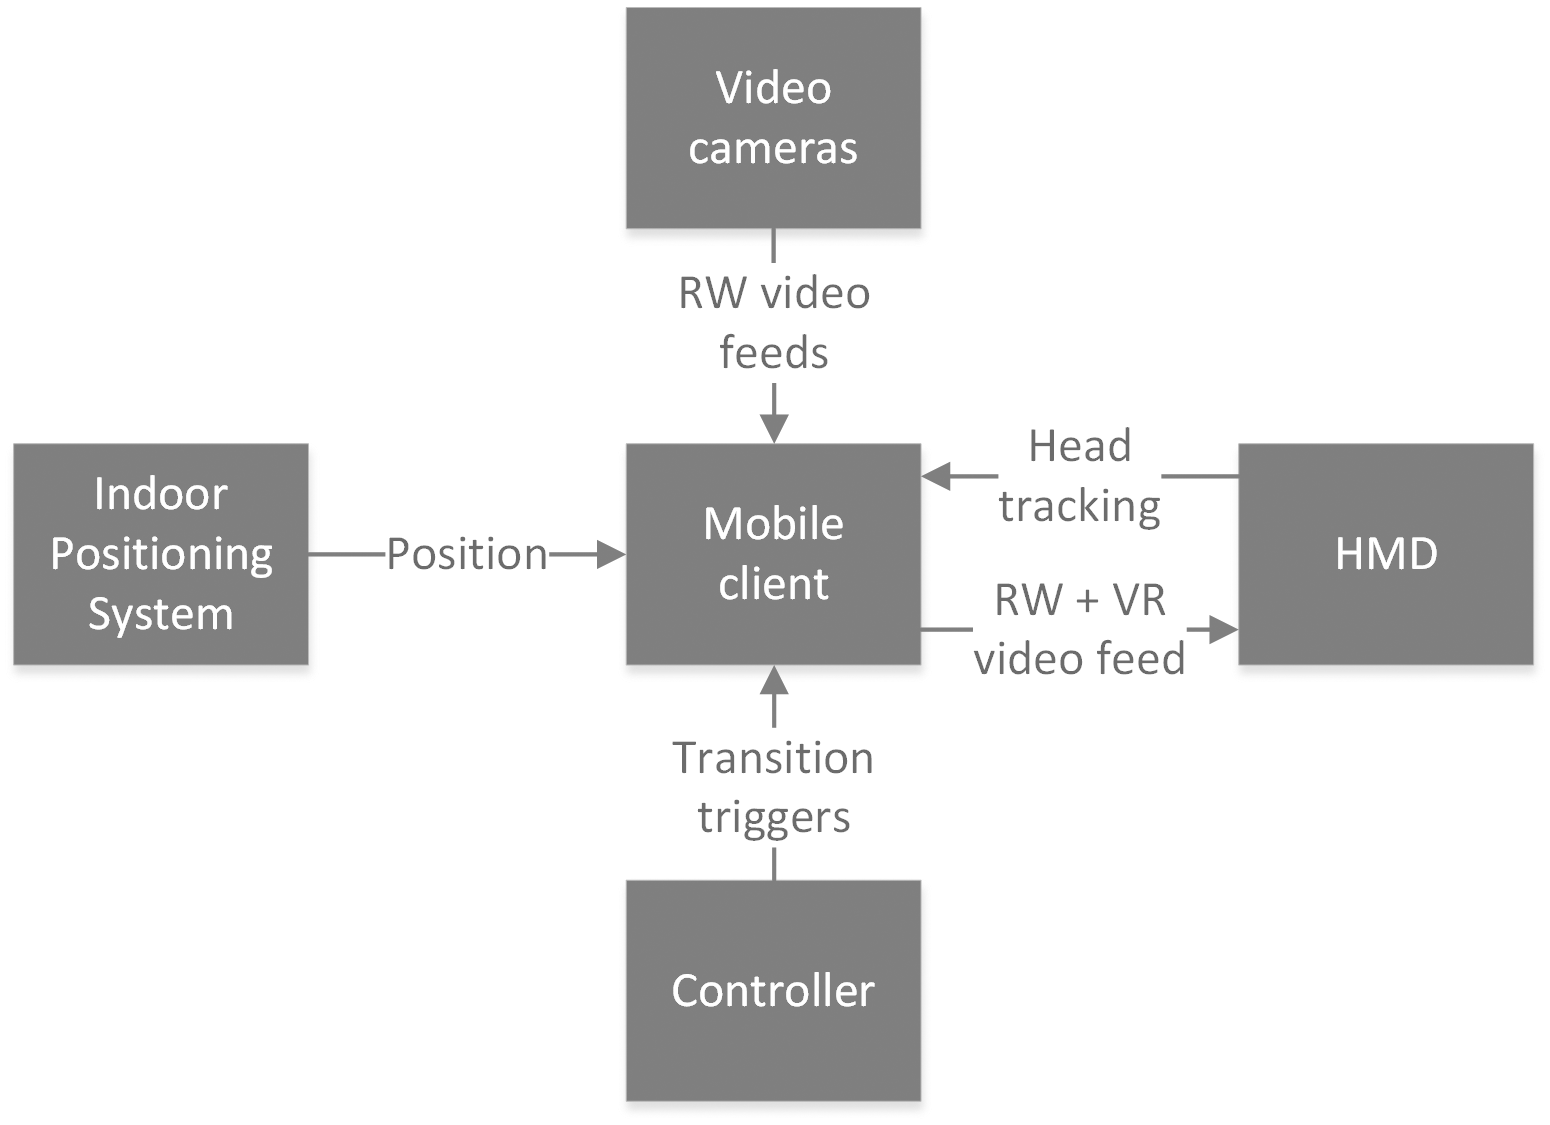
\includegraphics[width=.5\linewidth]{system-architecture.png}
		\caption{High level overview of the Mirrorshades parallel reality platform in use.}
		\label{systemarchitecture}
	\end{center}
\end{figure}

\begin{figure}[h]
	\begin{center}
		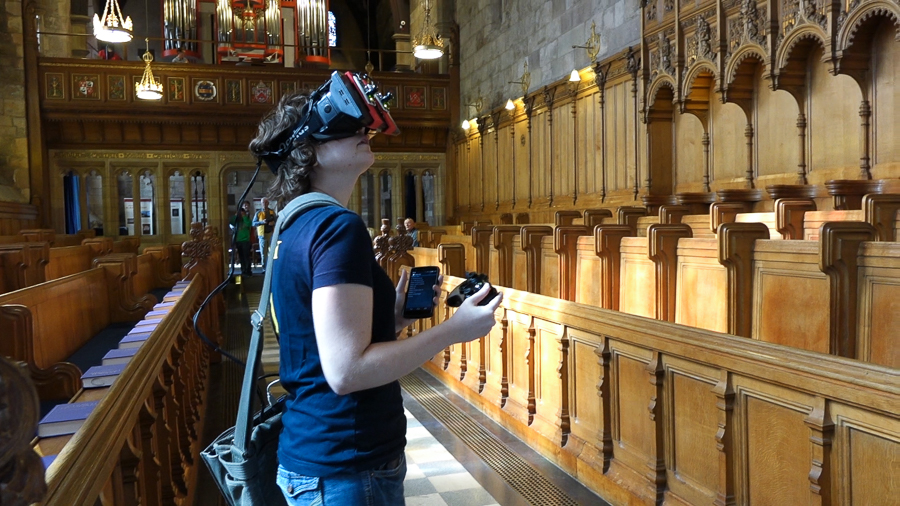
\includegraphics[width=\linewidth]{participant-f-5.jpg}
		\caption{The Mirrorshades parallel reality platform.}
		\label{participant-f-5.jpg}
	\end{center}
\end{figure}

Emphasis should be placed on the fact that the two views, RW and VR, through the function of the IPS and head tracking combined with the spatial equivalence of the constituent environments, represent equivalent vantage points within the two environments, differentiating the modality of interaction from the visual perception exchange systems exhibited in an Istanbul church by Mathieu Briand, which at first glance might have seemed to provide a similar modality at least in terms of the hardware employed and the use of a heritage scenario.

\begin{quote}
	\textit{``In an earlier version, set in the Hagia Eirene church in Istanbul, visitors wearing a wireless headgear viewing device could press a button to exchange the image on the screen with that of another of the six headgear cameras, revealing whatever it was pointing at. Visitors were fascinated by the dynamic visual transformations, such as the way the brightly painted floor could suddenly be replaced by the church dome as they wandered around the space.''}~\cite{Jones2006}
\end{quote}

Likewise the modality of interaction provided by the Mirrorshades platform distances itself from that of Briand's later experiments into `controlled schizophrenia' in which displacement of body and vision were intentional, as the different views that a user of the Mirrorshades platform switches between are inherently the same `place' as seen from the same vantage point.

\begin{quote}
	\textit{``The audience members wear helmets that incorporate a camera, goggle-style compact monitor, and headphones. The audience members may also carry a connector that can be plugged and unplugged from the nine sockets placed around the museum, in order to exchange audiovisual experiences with others.}

	\textit{When a connector is not plugged into a socket, one sees the environment through his/her own camera. In other words, one walks around seeing the surrounding environment through his goggle monitor. When the connector is plugged into a socket on the wall, the person sees the view taken by one of the three cameras installed in the building, or taken by another camera worn by another audience member whose camera is also connected to a socket.''}~\cite{Jones2006}
\end{quote}

%=========================================================================================================

\subsection{St Salvator's Chapel}

The cultural heritage site in mind when developing the Mirrorshades platform was St Salvator's chapel in St Andrews. Founded in 1450 but internally stripped of its medieval fittings during the Protestant Reformation (1517 - 1648) the chapel looks markedly different today than it did upon its completion. An existing virtual reconstruction of the chapel as it stood in the period 1450-1460, created by the OVW group, and the marked differences between the internal appearance of the reconstruction and the present day building (including the replacement of the original stone roof with a wooden one and drastically different dividing of the internal space) made the chapel an ideal candidate within the context of cultural heritage for the Mirrorshades parallel reality system to be deployed. The magnitude of the changes between the chapel's original state and how it stands today means that augmented reality would not in fact be able to present a faithful image of how the chapel originally looked, but would need to be combined with substantial application of diminished reality to remove present day features that were not there in the past. For example, when in proximity to the rood screen in its new position (discussed beneath), removing it would require replacing almost the entire viewport with augmented and diminished visuals.

\TwoFig{sallies-vrst/sallies-quad-real.jpg}{St Salvator's chapel today.}{sallies-quad-real.jpg}
       {sallies-vrst/sallies-quad-virtual.png}{St Salvator's chapel reconstruction.}{sallies-quad-virtual.png}
       
The chapel was of the greatest significance for the new architectural ideas that it introduced into Scotland, at a time when Scotland was particularly open to external artistic influences. However although the shell of the chapel survives and remains in use, it has lost its vault, its window tracery and its liturgical furnishings; it now requires specialist skills to appreciate the quality of its original state. As with other reconstructions from the OVW group, the virtual St Salvator's chapel was a product of a collaboration between architectural, art history and computer science scholarship. On the combined evidence of a highly detailed late medieval inventory and of the architecture itself, it has been possible to show how the chapel was furnished internally with altars, choir stalls, lecterns, screens, stained glass and wall paintings. The architectural, liturgical and spatial analysis allows our understanding of the history of the Chapel as a living building to be enormously enhanced by experiencing the building in its original context.

\TwoFig{sallies-vrst/sallies-real-toward-altar.jpg}{St Salvator's chapel looking East, present day (note lack of rood screen in this view).}{sallies-real-toward-altar.jpg}
       {sallies-vrst/sallies-virtual-toward-altar.png}{St Salvator's chapel looking East, reconstruction.}{sallies-virtual-toward-altar.png}

The chapel is an aisle-less rectangle with a three-sided east apse. Deeply projecting three-stage buttresses define the bays, which are now capped by pinnacles of 1861-2. The windows which occupy the full space available between the buttresses no longer reflect their original forms. The main entrance to the chapel was originally through a doorway in the second bay from the west of the south flank, which is covered by a vaulted porch between the buttresses. Two doorways on the north side presumably opened into a lost sacristy and treasury range.

The interior of the chapel is known to have been covered by a stone vault, which is assumed to have been of pointed barrel form with a decorative pattern of ribs, like the small vault over the south porch. The interior is now covered by an inappropriate timber roof.

\TwoFig{sallies-vrst/sallies-real-from-altar.jpg}{St Salvator's chapel looking West, present day.}{sallies-real-from-altar.jpg}
       {sallies-vrst/sallies-virtual-from-altar.png}{St Salvator's chapel looking West, reconstruction (note closer position of rood screen).}{sallies-virtual-from-altar.png}

St Salvator's chapel is considered the first Scottish example of a church planned with an aisle-less rectangular main body terminating in a polygonal eastern apse, a type that was to have a long future for a range of Scottish church types. Such chapels were common in university colleges in France and since Bishop Kennedy had a highly placed kinsman in the university of Paris and drew many ideas for the organisation of his college from that university's constitution, it is reasonable to assume that he also drew some of his ideas for the architecture of his chapel from there. On this basis, St Salvator's chapel must be seen as an outstandingly important channel for the introduction into Scotland of new architectural ideas from France. The new architecture made a significant statement in its Scottish context. 

The reconstruction of the chapel involved both the mental reconstruction of modified and lost features, and the establishment of the range of ways in which buildings that represent a spirituality alien to modern students were intended to function. As such it offers an invaluable academic discipline for those involved in the reconstruction, providing eminently practical ways of testing theories and assumptions. The development of a parallel reality system which enables comparison between the real and virtual chapel in the same time and place aimed to further enhance the value of the existing reconstruction.

%=========================================================================================================

\section{Virtual Reality HMD}
The concept of virtual reality and the associated HMDs that provide wide field of view, stereoscopic 3D graphics coupled with head tracking is currently experiencing a resurgence of interest and investment, thanks largely to the advent of Oculus\footnote{\url{https://www.oculus.com/}} and their Rift platform\footnote{\url{https://www.oculus.com/rift/}}. Whilst the first head mounted computer display was created in the late 1960s by Ivan Sutherland~\cite{Rheingold1992}, it was not until the late 1980s and early 1990s that VR began to be promoted as a consumer platform. Unfortunately both hardware and software were not ready for consumer adoption at this time and these systems failed to live up to the substantial hype of being a \textit{``revolutionary technology''} which promised to \textit{``transform society''} (figure \ref{rheingold-virtual-reality.jpg}), resulting in the VR bubble bursting.

\begin{figure}[h]
	\begin{center}
		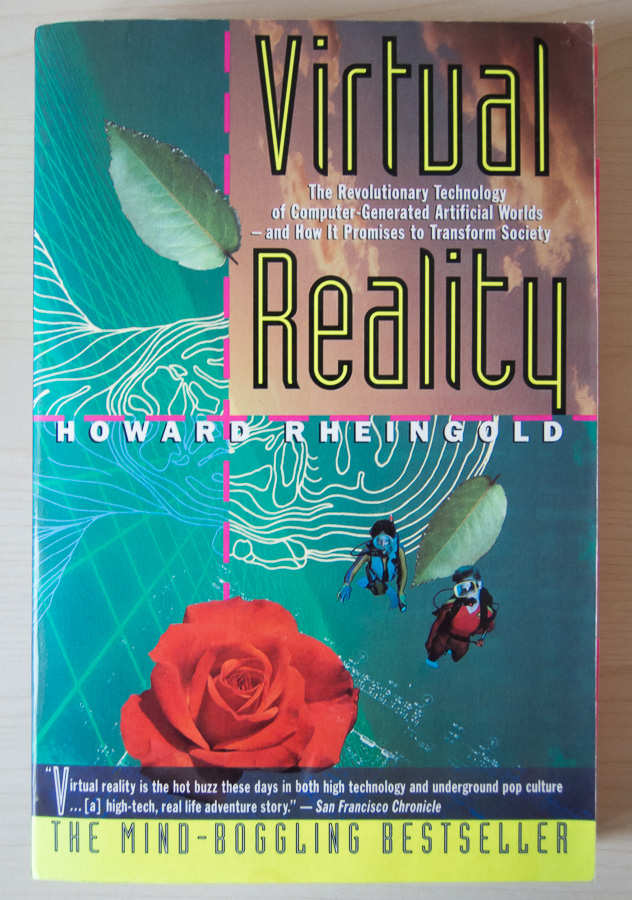
\includegraphics[width=0.4\textwidth]{rheingold-virtual-reality.jpg}
		\caption{Howard Rheingold's 1992 bestseller \textit{Virtual Reality}.}
		\label{rheingold-virtual-reality.jpg}
	\end{center}
\end{figure}

Decades after this initial disappointment with consumer centric VR, Oculus now looks set to finally begin realising a successful consumer VR platform thanks largely to the substantial advances in display technologies made during the past decade driven primarily by the explosive popularity of smartphones and tablets. Pre-Oculus HMDs predominantly made use of two separate microdisplays, one for each eye; Sutherland's original `Sword of Damocles' made use of two tiny CRT screens, whilst later HMDs made use of two OLED microdisplays. As the number of market applications for microdisplay technology was (\& continues to be) relatively small, there are limited microdisplay models to chose between and they command high price points when considering integration into consumer products.

Oculus have taken a different approach for their Rift Developer Kit HMDs. Instead of using two small displays, one for each eye, they use a single larger display upon which two separate images are rendered, side-by-side. This approach has two distinct advantages compared to prior dual microdisplay techniques. Firstly the complexity of the device is reduced, which positively impacts price, ease of integration and content development methodologies. Secondly the cost of a single display in the 5"-7" range is drastically lower than the cost of a pair of microdisplays, thanks to the surging popularity of smartphones and tablet computers in this size range. By making use of readily available displays intended for the smartphone/tablet market, Oculus were able to bring their first Development Kit (DK1) to market for researchers and enthusiasts at a price of only \$300, while still providing substantially wider FOV than the vast majority of existing HMDs - even those commanding substantially higher price points.

For comparison, examples of consumer-grade commercial HMDs that use the twin OLED microdisplay approach, the Sony HMZ-T1 which launched with a price of \textyen60,000 (\$800 at exchange rates of the time) and its successor the HMZ-T2 which launched with a price of \textyen70,000 (\$900 at exchange rates of the time), provide $45$\textdegree\ horizontal/$51.6$\textdegree\ diagonal FOV and no head tracking (intended primarily as a personal 3D cinema experience). Oculus' DK1 provides more than $90$\textdegree\ horizontal and $110$\textdegree\ diagonal FOV and integrates a head tracking solution operating at a rate of 1kHz and providing best in class accuracy. Combined with advances in both hardware and software tasked with producing 3D graphics, the user experience of Oculus' HMD offerings is promising to finally deliver on the VR hype of the 90s.

The March 2014 acquisition of Oculus by Facebook\footnote{\url{https://www.facebook.com/zuck/posts/10101319050523971}} for \$2 billion\footnote{\url{http://www.theguardian.com/technology/2014/jul/22/facebook-oculus-rift-acquisition-virtual-reality}} and Oculus partnership with Samsung, one of the world's leading display manufacturers and which has already led to the release of an innovative VR HMD that makes use of an existing smartphone as its display\footnote{\url{https://www.oculus.com/gear-vr/}}, lends hope that this wave of VR excitement will be met with success where its hype-laden 90s counterpart was met with failure.

%\textbf{***Maybe talk about what other HMDs there were actually available to me on the market? Vuzix 1200/900/whatever?}

%take bits from that youtube video from Samsung developers?

%=========================================================================================================

\subsection{The Oculus Rift DK1 and Unity Game Engine}

The OVW group took delivery of an Oculus Rift DK1 from the first batch of units shipped to the EU in August 2013. The immersive experience of using the DK1, thanks to its wide FOV, fast and accurate head tracking, stereoscopic 3D and novelty compared to traditional 2D displays, presented a markedly different modality of interaction with virtual content than the 10'' display of the tablet used by VTW. By filling the user's entire field of view with whatever visuals are displayed upon its screen, the Rift allowed for investigation of the true essence of the experiential aspect of wholly switching between real and virtual environments that the parallel reality concept envisioned.

At this early stage after the DK1's release, the best supported software platform in terms of API provision and integration was the Unity game engine. After experience with modifying the Second Life client as part of the VTW project, it was decided best to convert the OVW group's OpenSim model of St Salvator's chapel into a Unity compatible format rather than embarking upon further modification to the Second Life client to support the DK1. Since the development of VTW the OVW group successfully engineered an automated process for converting OpenSim content into Unity compatible content, allowing the group's existing content, such as the chapel model, to be deployed within Unity executables.

One deciding factor in opting to convert OpenSim content to Unity rather than use the content in its original OpenSim setting was the more stringent performance requirements for an enjoyable VR HMD experience compared to those of a traditional desktop/handhend display experience. When using a HMD such as the DK1, a smooth, high framerate is required to avoid a kind of motion sickness referred to as `simulator sickness'. Oculus' official guidelines are for Rift applications to \textit{``run at a frame rate equal to or greater than the Rift display refresh rate''}\footnote{\url{http://static.oculus.com/sdk-downloads/documents/Oculus_Best_Practices_Guide.pdf}} which in the case of the DK1 is 60Hz. Due to the possibly ephemeral nature of Second Life/OpenSim content where users are free to create, modify and destroy content in real time, Second Life as a 3D platform suffers in terms of performance compared to game engines such as Unity due to not being able to exploit techniques such as occlusion culling~\cite{willmott:largecomplex} which require an offline processing phase that depends upon environmental content remaining unchanged throughout deployment. The OVW group's experience in presenting Second Life/OpenSim content on a range of different hardware did not point to good odds of managing to render the St Salvator's chapel scene at close to 60fps, especially considering the overhead introduced by stereoscopic rendering even where the total resolution of the two side-by-side images is no greater than the single equivalent monoscopic image. As Mirrorshades is a mobile application and the computer producing the visuals was to be carried by the user, the hardware specification of this client were limited compared to those that the group had used in alternative static deployments.

%=========================================================================================================

\subsection{Modifying the DK1 for Video See-Through}
\label{modifying-dk1}
The Oculus Rift DK1 covers the user's entire field of view, such that they cannot see any of their real world surroundings whilst wearing it, and it does not feature any camera provision to allow a mediated view of the real world to be presented to them. As such it was necessary to modify the DK1 to imbue it with video see-through capability for use as a component of the Mirrorshades parallel reality platform. When choosing cameras for this task there were several desired features:
\begin{itemize}
	\item Resolution and refresh rate that match (or exceed) each half of the DK1's display.
	\item Sensor aspect ratio that matches that of each half of the DK1's display.
	\item Lens focal length and sensor dimensions that provide wide FOV (ideally matching the FOV of the DK1).
	\item Ease of integration with the Unity platform.
	\item Price realistic for a virtual heritage deployment.
\end{itemize}

The \$300 price tag of the DK1 and the low price of consumer webcams for computer and console use met with the budgetary requirement of the video see-through solution. The PS3 Eye camera met most of the technical requirements and has a history of use in computer vision research scenarios as part of the PS Move motion sensing platform (see section \ref{psmove}). While its resolution of 640x480 pixels does not meet each half of the DK1's display at 640x800 pixels, unusually for a USB camera it is capable of running at 60fps - the refresh rate of the DK1. The aspect ratio of the 640x480 sensor is 4:3, which although not identical to the 5:4 aspect ratio of each eye's 640x800 half of the DK1 screen, is closer than the 16:10 or 16:9 aspect ratio of a `widescreen' camera sensor. Furthermore once dismantled to its bare PCB it features mounting holes for a standard S-mount (M12x0.5mm) lens mount commonly used for CCTV cameras, allowing alternative focal length lenses to be easily fitted.

An early test with the PS3 Eye and the DK1 (a video of which is available to view online\footnote{\url{https://www.youtube.com/watch?v=tS0FGZxQzCU}}) was performed by simply attaching a single unmodified PS3 Eye camera to the top of the DK1 (figure \ref{rift-pseye-ziptied.jpg}) with its stock lens set to its `wide' setting (75\textdegree, presumably diagonal, FOV\footnote{\url{http://uk.playstation.com/media/247868/7010571 PS3 Eye Web_GB.pdf}}). This test evaluated the suitability of Unity's \texttt{WebCamTexture}\footnote{\url{http://docs.unity3d.com/ScriptReference/WebCamTexture.html}} feature for integrating the stream from a USB camera into a 3D application. For this test the mediated RW video stream was rendered to a small `floating' window that moved with the user's head (figure \ref{floating-webcam-window.png}) allowing the user to perceive both environments simultaneously within the same viewport in a manner similar to VTW but in reverse - the virtual environment filling most of the viewport and the real environment as a smaller window in the periphery. Subsequently the camera streams were changed so as to render to the full expanse of the DK1's display, to better realise the switching experiential vision of parallel reality.

\TwoFig{rift-pseye-ziptied.jpg}{Oculus Rift DK1 with PS3 Eye.}{rift-pseye-ziptied.jpg}
       {floating-webcam-window.png}{`Floating' window video see-through in Unity.}{floating-webcam-window.png}

A pair of PS3 Eye cameras were dismantled, their outer plastic housing removed, stock lenses removed and S-mount lens mounts fitted. Ideally the lenses used would provide the same FOV that the Rift itself is capable of displaying, such that the mediate RW streams from the cameras could be displayed at the full size of the Rift and `match' the FOV of whatever virtual content was alternatively displayed. However there is a trade off with lenses between focal length and distortion: shorter focal lengths mean a wider FOV, however they also introduce more distortion which is not necessarily corrected by the shader that the Rift uses to compensate for the distortion of its own plastic lenses through which its display viewed.

The PS3 Eye camera has a `1/4'' type' sensor but this classification is only an indication of its true dimensions\footnote{\url{http://www.dpreview.com/glossary/camera-system/sensor-sizes}}. As Sony has not published the actual dimensions of the sensor the typical 1/4'' type dimensions\footnote{\url{http://www.photoreview.com.au/tips/buying/unravelling-sensor-sizes}} of 4.5mm diagonal, 3.6mm horizontal, 2.7mm vertical were adopted for calculating FOV estimations. Table \ref{fov-table} gives the diagonal, horizontal and vertical FOV of the shortest focal length S-mount lenses readily available. Empirical accounts of very short focal length S-mount lenses mounted to the PS3 Eye camera indicated that the distortion becomes very high beneath 2.1mm\footnote{\url{http://peauproductions.com/store/index.php?main_page=index&cPath=26_4}}. Whilst 1.7mm lenses would provide almost identical FOV to the Rift's display (105.9\textdegree\ diagonal for the cameras, 110\textdegree\ diagonal for the Rift) the amount of distortion introduced would likely be of such an extent that the experience of viewing the mediate RW environment would be degraded more by distortion than by the limited/non-matching FOV of longer focal length lenses.

\begin{table}
\begin{center}
\begin{tabularx}{\textwidth}{c *{4}{>{\centering\arraybackslash}X}}
\toprule
\textbf{Focal length (mm)} & \textbf{Diagonal FOV (\textdegree)} & \textbf{Horizontal FOV (\textdegree)} & \textbf{Vertical FOV (\textdegree)} \\
\midrule
2.5mm & 84    & 71.5 & 56.7 \\
2.1mm & 93.9  & 81.2 & 65.5 \\
2.0mm & 96.7  & 84   & 68 \\
1.9mm & 99.6  & 86.9 & 70.8 \\
1.8mm & 102.7 & 90   & 73.7 \\
1.7mm & 105.9 & 93.3 & 76.9 \\

\bottomrule

\end{tabularx}
\caption{FOV of various focal length lenses resolving onto a 1/4'' type sensor.}
\label{fov-table}
\end{center}
\end{table}

However using a lens with a focal length short enough to provide a FOV as wide as the Rift was discovered to not be strictly necessary, as when wearing the Rift the edges of the image presented to each eye are not always visible to the user. This is especially true where the Rift's adjustable eye relief is set such that it sits at its furthest position. Such an adjustment is actually prudent for user study conditions, as using the Rift at its maximum eye relief ensures the best compatibility and comfort with users and also removes a variable between users that would be introduced if each were permitted to chose the relief themselves. Thus the choice of lens could be dictated by identifying the FOV required to fill the portion of the Rift's images that were visible when the eye relief was set to its maximal position, rather than by matching the Rift's overall FOV. This allowed the use of lenses with focal length long enough that the distortion they introduced was not so bad as to require a separate correction phase in software rendering.

Experiments revealed that with the DK1 set to its maximum relief, the area of the images visible to the user was wider than that provided by 2.5mm lenses (84\textdegree\ diagonal) when scaled correctly and narrower than that provided by 2.1mm lenses (93.9\textdegree\ diagonal) when scaled correctly. With no availability of lenses with a focal length between 2.5mm and 2.1mm, the 2.1mm focal length was adopted. Figure \ref{lens-comparison-on-ps3eye-pcb.jpg} shows the 2.5mm lens (right) and 2.1mm lens (left) mounted to the PS3 Eye PCBs via S-mount lens mounts, while figure \ref{fov-comparison-1.png} shows the FOV of the selected 2.1mm lenses scaled correctly upon the wider FOV of the DK1's images showing a scene within St Salvator's chapel.

\TwoFig{rift-clips-cameras/lens-comparison-on-ps3eye-pcb.jpg}{S-mount lenses on PS3 Eye camera PCBs.}{lens-comparison-on-ps3eye-pcb.jpg}
       {fov-comparison-1.png}{FOV comparison between DK1 and 2.1mm lenses.}{fov-comparison-1.png}

%{fov-comparison-2.png}{}{fov-comparison-2.png}

The PS3 Eye cameras were mounted to the DK1 by modifying the 3D printable sensor mount design released by the University of Southern California Institute for Creative Technologies\footnote{\url{http://projects.ict.usc.edu/mxr/diy/oculus-sensor-mount/}}. The modified mount comprised a base piece (figure \ref{clips.jpg}) that clipped securely over the front of the DK1 and a slotted plate (figure \ref{clips-hori-plate.jpg}) onto which the PS3 Eye cameras were mounted. These parts were 3D printed using a MakerBot Replicator 2X\footnote{\url{http://store.makerbot.com/replicator2x}} and combined using epoxy resin. The combination is shown attached to the DK1 in figure \ref{hori-1.jpg}. The slots in the slotted plate were spaced to match the mounting holes of the PS3 Eye PCB, such that the cameras could be attached by metal stand-offs (figure \ref{hori-2.jpg}) allowing horizontal adjustment to alter the distance between them to account for different interpupillary distances. Figure \ref{hori-3.jpg} shows how one camera was mounted `upside down' to allow enough clearance between the PCBs to accommodate small interpuillary distances.

\begin{figure}[h]
    \centering
    \begin{minipage}{.32\textwidth}
        \centering
        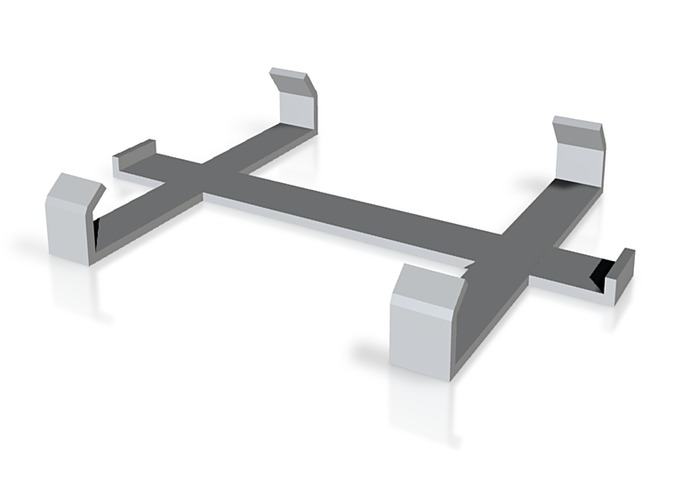
\includegraphics[width=\textwidth]{rift-clips-cameras/clips.jpg}
        \caption{Camera mount base.}
        \label{clips.jpg}
    \end{minipage}%
    \hspace{.01\textwidth}
    \begin{minipage}{0.32\textwidth}
        \centering
        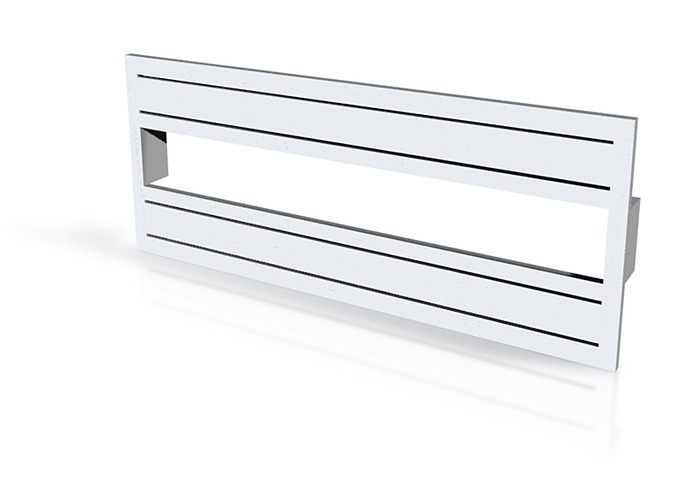
\includegraphics[width=\textwidth]{rift-clips-cameras/clips-hori-plate.jpg}
        \caption{Camera mount slotted plate.}
        \label{clips-hori-plate.jpg}
    \end{minipage}%
    \hspace{.01\textwidth}
    \begin{minipage}{0.32\textwidth}
        \centering
        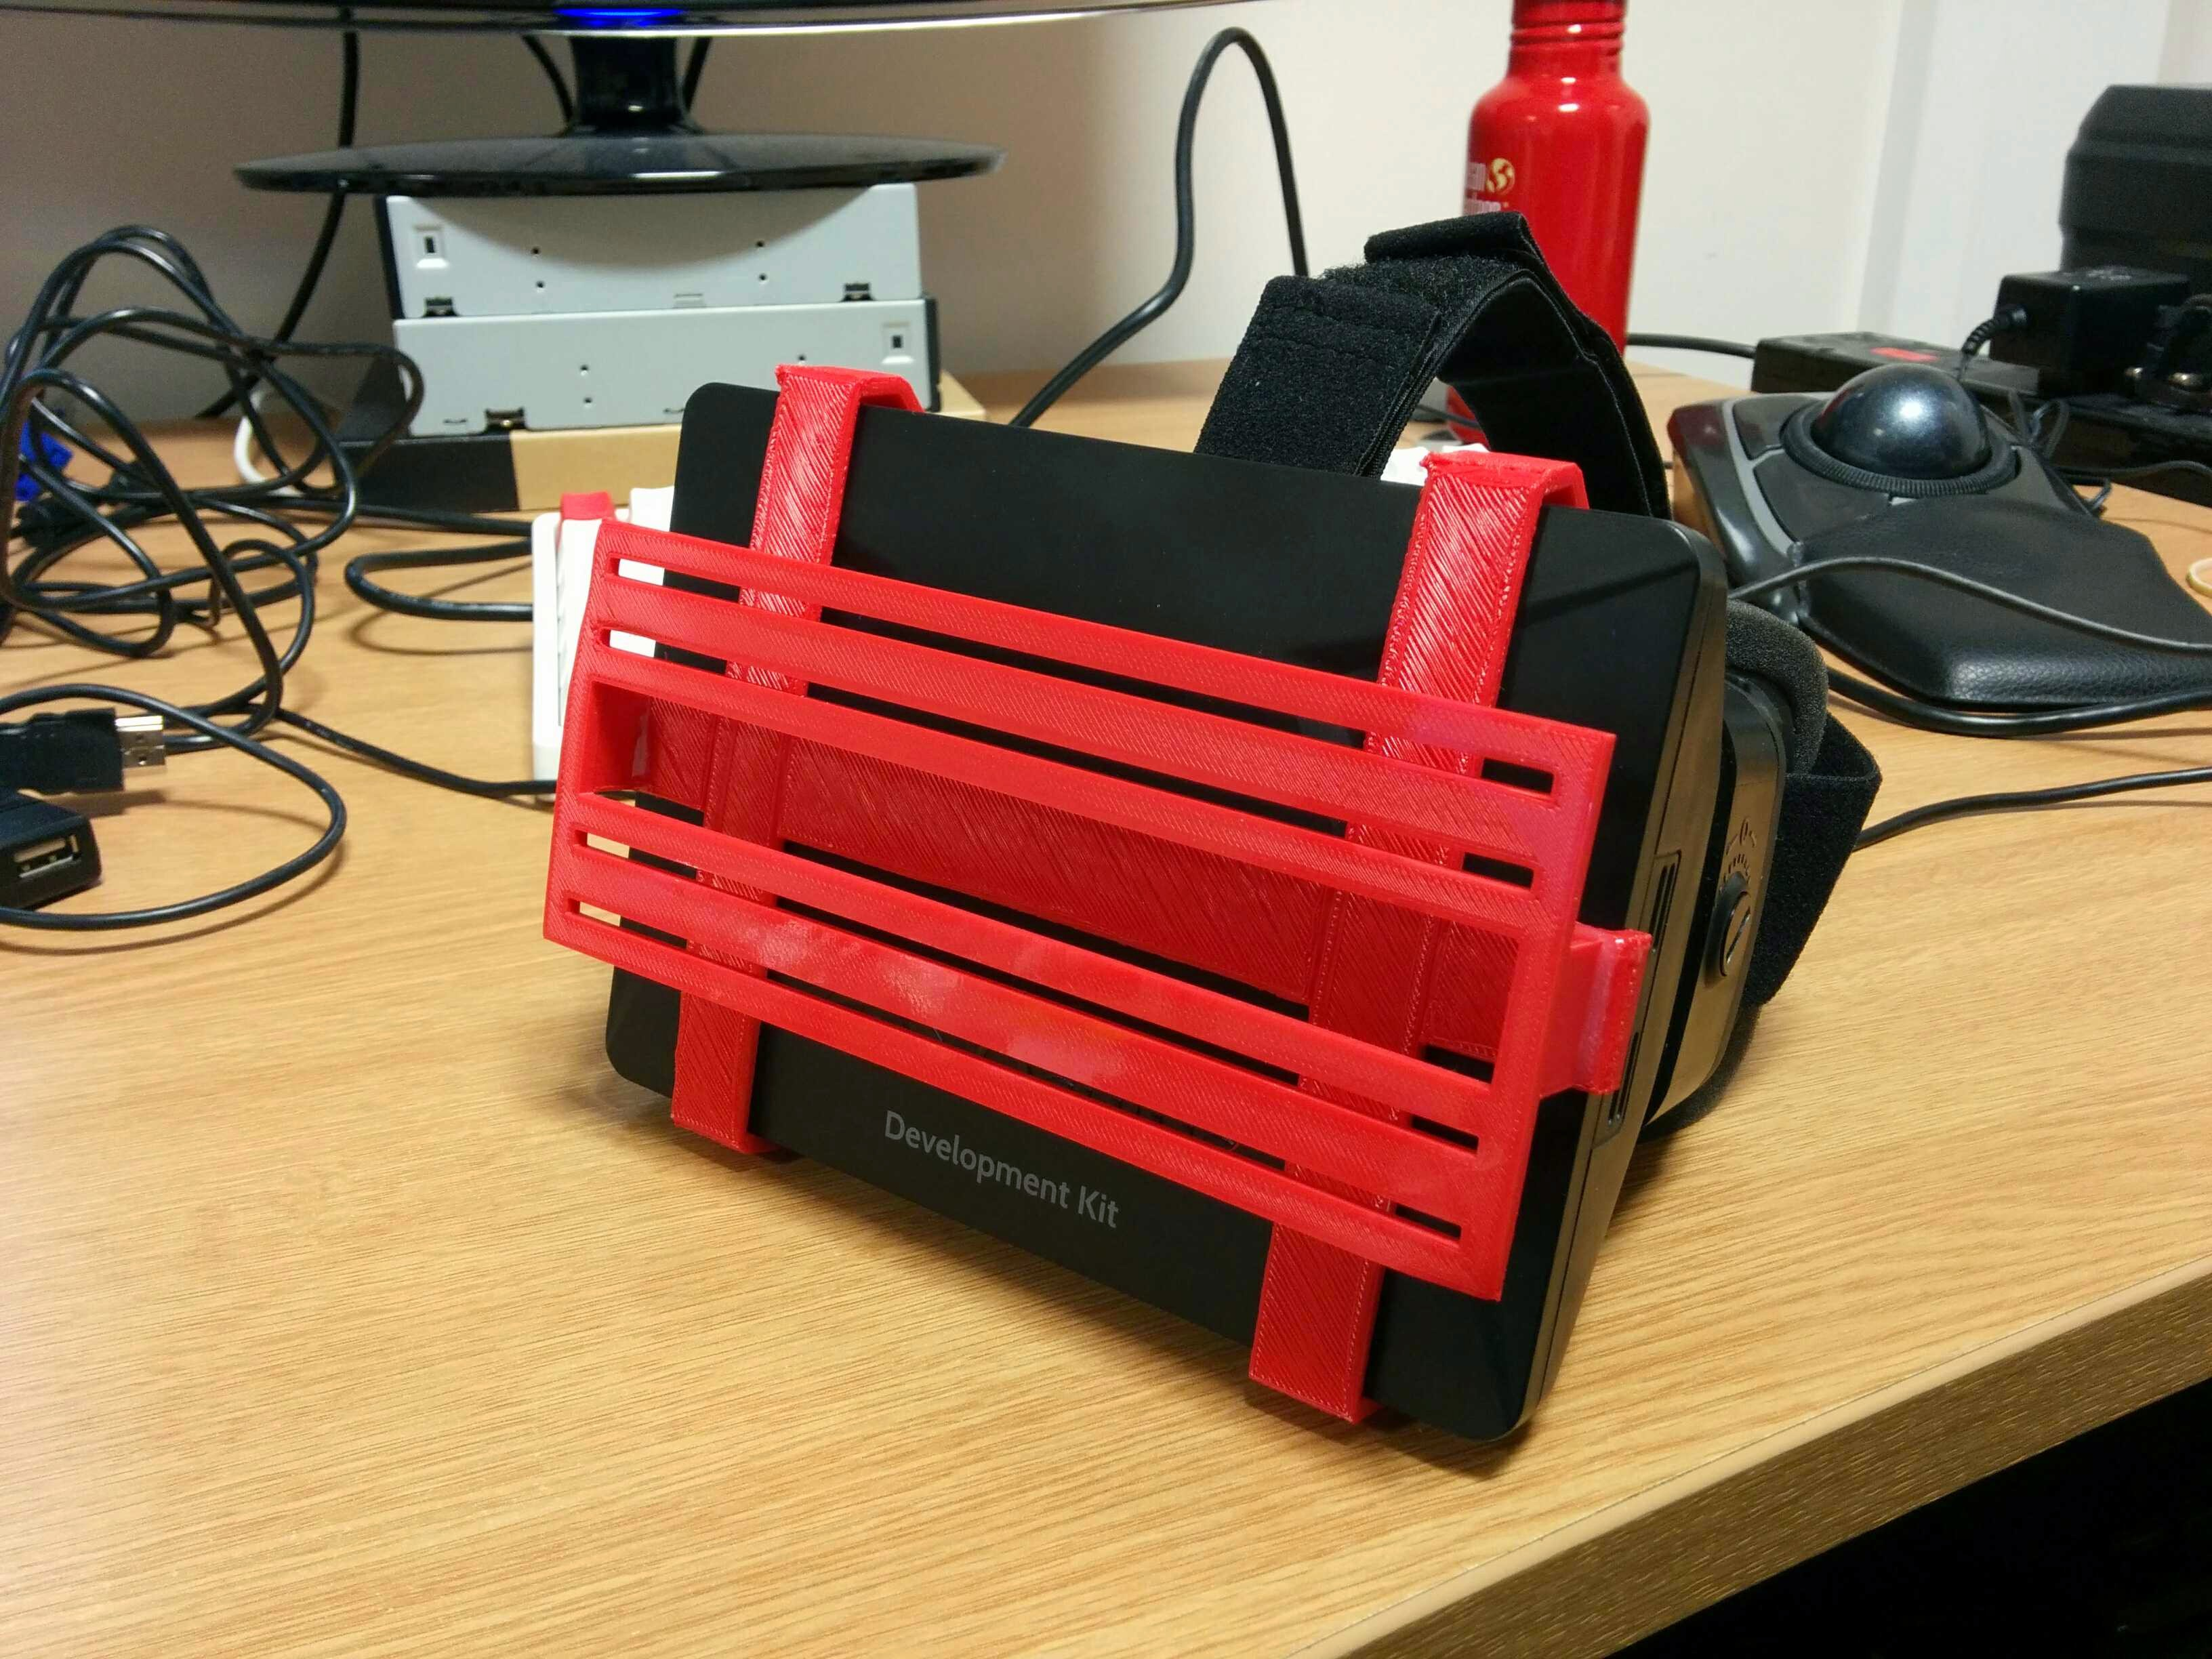
\includegraphics[width=\textwidth]{rift-clips-cameras/hori-1.jpg}
        \caption{Camera mount attached to DK1.}
        \label{hori-1.jpg}
    \end{minipage}
\end{figure}

\TwoFig{rift-clips-cameras/hori-2.jpg}{Cameras mounted using stand-offs.}{hori-2.jpg}
       {rift-clips-cameras/hori-3.jpg}{Two PS3 Eye cameras mounted on DK1.}{hori-3.jpg}

An oversight in the design of the camera mounts was realised when William Steptoe subsequently released details of his `AR Rift' project~\cite{Steptoe2014}. Although the DK1's overall screen has a resolution of 1280x800 in a landscape 16:10 aspect ratio, each half of this screen as presented individually to each eye has a resolution of 640x800 in a portrait 4:5 aspect ratio. Thus to best match the aspect ratio of a 4:3 camera sensor such as that of the PS3 Eye to each half of the DK1's screen, that camera should be oriented in a portrait orientation rather than the landscape orientation that had been employed thus far by the Mirrorshades platform with the PS3 Eye cameras. New mounting hardware was designed and printed by further modification of the USC's original 3D designs in order to vertically mount the PS3 Eye cameras. This new design is shown in figure \ref{clips-vert.jpg} (the recessed section in the centre of the clip allows for the heads of bolts to clear the front of the DK1) and the assembled units are shown attached to the DK1 in figure \ref{vert-6.jpg}. The files for printing both versions of the camera mounts are available online\footnote{\url{https://github.com/CJ-Davies/Oculus-Rift-DK1-camera-mounts}}. Additionally the metal stand-offs that had been used to mount the camera PCBs to the clips (figure \ref{vert-1.jpg}) were replaced with a combination of rubber washers and threaded bolts (figure \ref{vert-4.jpg}) both to reduce the discrepancy in the mediated RW images caused by the distance between the camera sensors and the user's eyes (by reducing this distance) and to allow for finer alteration of the orientation of the cameras.

\TwoFig{rift-clips-cameras/clips-vert.jpg}{Updated camera mount.}{clips-vert.jpg}
       {rift-clips-cameras/vert-6.jpg}{PS3 Eye cameras using updated mounts.}{vert-6.jpg}

\TwoFig{rift-clips-cameras/vert-1.jpg}{Updated camera mount with stand-offs.}{vert-1.jpg}
       {rift-clips-cameras/vert-4.jpg}{Updated camera mount with rubber washers.}{vert-4.jpg}

Although the initial integration test with a single PS3 Eye camera revealed its easy accessibility within Unity, using two PS3 Eye cameras proved temperamental. Unity's \texttt{WebCamTexture} support identifies webcams via their `name' as provided by their driver. In the case of the PS3 Eye using the driver provided by Code Laboratories\footnote{\url{https://codelaboratories.com/products/eye/driver/}} (this third party driver was required as no official Windows driver is available from Sony, as the PS3 Eye was only marketed for use with the PS3 console) an issue arose where both cameras presented the same name to Unity and the second camera overwrote the reference to the first, only allowing access to a single camera. Figure \ref{ps3-eye-unity-overwrite.png} shows this issue, that whilst Windows' device manager successfully identified both cameras independently, Unity's \path{WebCamTexture.devices()} function returned a reference to only one (the \texttt{BisonCam, NB Pro} entry is the laptop's internal webcam). A partial solution to this issue was presented by a community provided Unity package\footnote{\url{http://tips.hecomi.com/entry/20130731/1375279561} (Japanese)} which allowed the setup up to be successfully tested within a departmental building, a video of which is available to view online\footnote{\url{https://www.youtube.com/watch?v=oy5NqqDtkJ4}}.

\begin{figure}[h]
	\begin{center}
		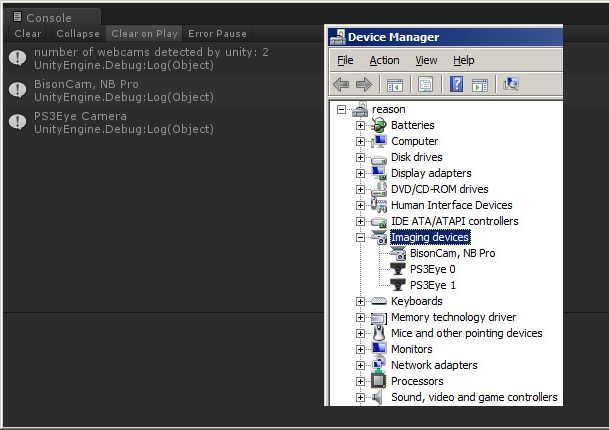
\includegraphics[width=.8\linewidth]{ps3-eye-unity-overwrite.png}
		\caption{Unity failing to instantiate references to multiple PS3 Eye cameras.}
		\label{ps3-eye-unity-overwrite.png}
	\end{center}
\end{figure}

Unfortunately this naming solution was temperamental at best and two camera compatibility was frequently lost, so the PS3 Eye cameras were scrapped. Using Steptoe's project as a guide, a pair of Logitech C310\footnote{\url{http://www.logitech.com/en-gb/product/hd-webcam-c310}} cameras were sourced. Whilst the refresh rate of the C310 is only 30Hz, half that of the PS3 Eye, it supports a resolution of 1280x960 which is higher than that of the PS3 Eye and of each half of the DK1's display. The switch from the PS3 Eye cameras to the C310 represented a sacrifice in terms of framerate but a gain in terms of resolution. Empirically the increase in resolution was indiscernible, likely due to the effect of the DK1's optics in reducing the visual acuity of its display, whilst the reduction in framerate was noticeable. However the reliable operation of the C310 made them the superior option compared to the temperamental status of the PS3 Eye, which would have made it impossible to perform user studies due to frequent and unpredictable failures.

The C310 cameras received the same attention as the PS3 Eye cameras: they were dismantled and outfitted with S-mount lens mounts. As the sensor in the C310 is also of the 1/4" type the FOV provided by the 2.1mm lenses on the C310 cameras is comparable to that of the same lenses mounted to the PS3 Eye cameras. Due to the lack of mounting holes present on the C310 PCB they were set into a thin sheet of thermoplastic (figure \ref{thermoplastic.jpg}) which was then attached to the 3D printed clips with the same rubber washer and threaded bolt arrangement as the PS3 Eye cameras. The assembled DK1 + dual C310 solution is shown by figures \ref{vert-7.jpg} (3/4 view), \ref{middle.jpg} (profile view) and \ref{right.jpg} (detail view).

\TwoFig{rift-clips-cameras/thermoplastic.jpg}{Setting C310 PCBs into thermoplastic.}{thermoplastic.jpg}
       {rift-clips-cameras/vert-7.jpg}{C310 mounted to DK1 (three-quarter view).}{vert-7.jpg}

\TwoFig{rift-clips-cameras/middle.jpg}{C310 mounted to DK1 (front view).}{middle.jpg}
       {rift-clips-cameras/right.jpg}{C310 mounted to DK1 (detail view).}{right.jpg}

%=========================================================================================================

\subsection{Switchable Stereoscopic Video See-Through with Unity}

Unity's \texttt{WebCamTexture} support was used to gain access to the C310 video streams within Unity: due to better provisioned drivers there was no issue with Unity obtaining references to both C310 cameras as there was with the two PS3 Eye cameras. These video streams are applied to a pair of planes, of matching orientation and aspect ratio to the video stream, that are situated perpendicular to the two virtual camera objects of the Oculus Unity prefab. This is shown by figure \ref{unity-screenshot-1.png} in which the smaller portrait planes in the centre of the image are those onto which the camera streams are rendered.

\begin{figure}[h]
    \begin{center}
    \begin{minipage}[t]{.32\textwidth}
        \begin{center}
        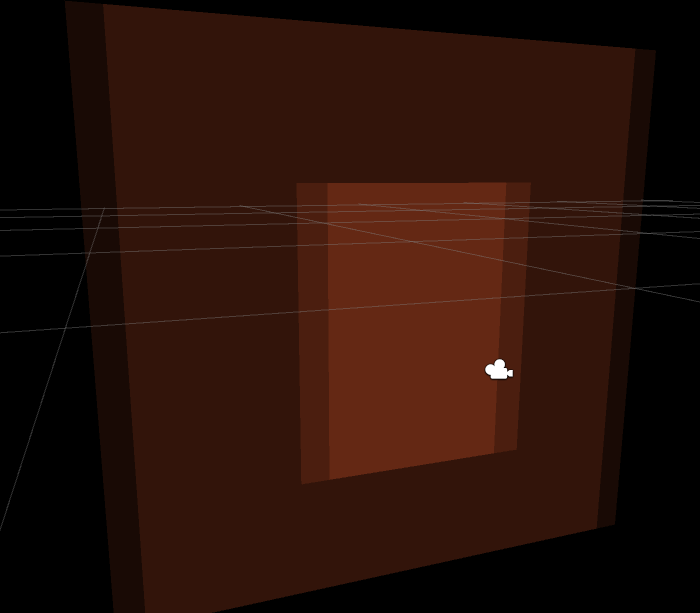
\includegraphics[width=\textwidth]{unity-screenshots/unity-screenshot-1.png}
        \caption{Camera and backing planes in Unity.}
        \label{unity-screenshot-1.png}
        \end{center}
    \end{minipage}%
    \hspace{.01\textwidth}
    \begin{minipage}[t]{.32\textwidth}
		\begin{center}
        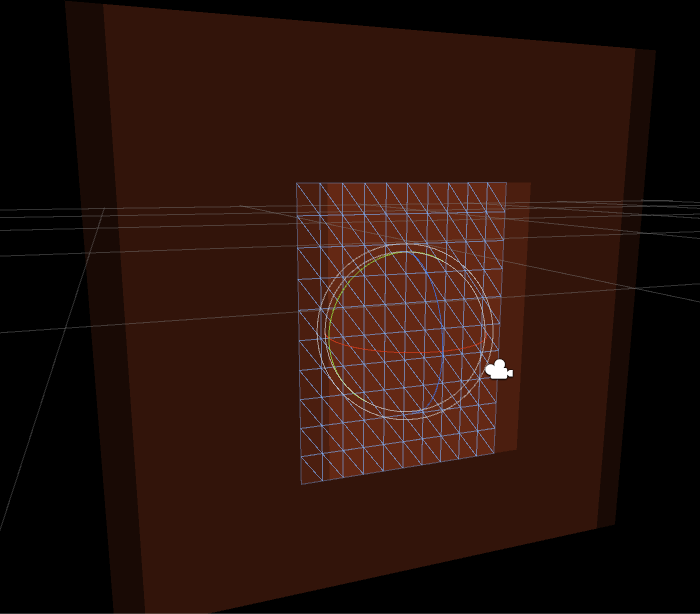
\includegraphics[width=\textwidth]{unity-screenshots/unity-screenshot-2.png}
        \caption{Left camera plane in Unity.}
        \label{unity-screenshot-2.png}
        \end{center}
    \end{minipage}%
    \hspace{.01\textwidth}
    \begin{minipage}[t]{.32\textwidth}
        \begin{center}
        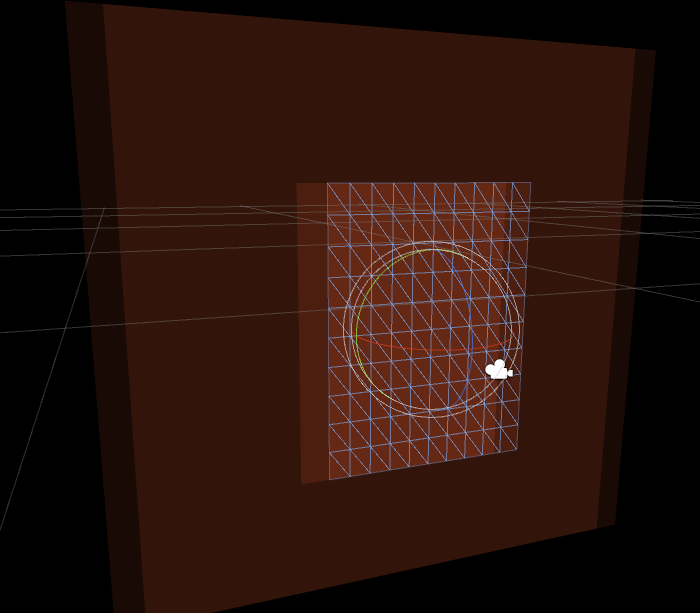
\includegraphics[width=\textwidth]{unity-screenshots/unity-screenshot-3.png}
        \caption{Right camera plane in Unity.}
        \label{unity-screenshot-3.png}
        \end{center}
    \end{minipage}
    \end{center}
\end{figure}

It can be seen that these planes overlap considerably as they are only horizontally spaced the same amount as the virtual cameras are spaced (see also figure \ref{webcam-overlap.png}), which is derived from the interpupillary distance that the user inputs to the Oculus configuration utility. By placing each of these two planes in a separate layer and setting the culling mask of the virtual cameras to cull/not-cull these layers appropriately (such that the left virtual camera culls the layer of the right plane but not the left plane and the right virtual camera culls the layer of the left plane but not the right plane) the appropriate virtual camera only sees the appropriate webcam image even though they overlap. The left virtual camera sees only the camera plane shown highlighted in figure \ref{unity-screenshot-2.png} while the right virtual camera sees only the camera plane shown highlighted in figure \ref{unity-screenshot-3.png}.

\begin{figure}[h]
	\begin{center}
		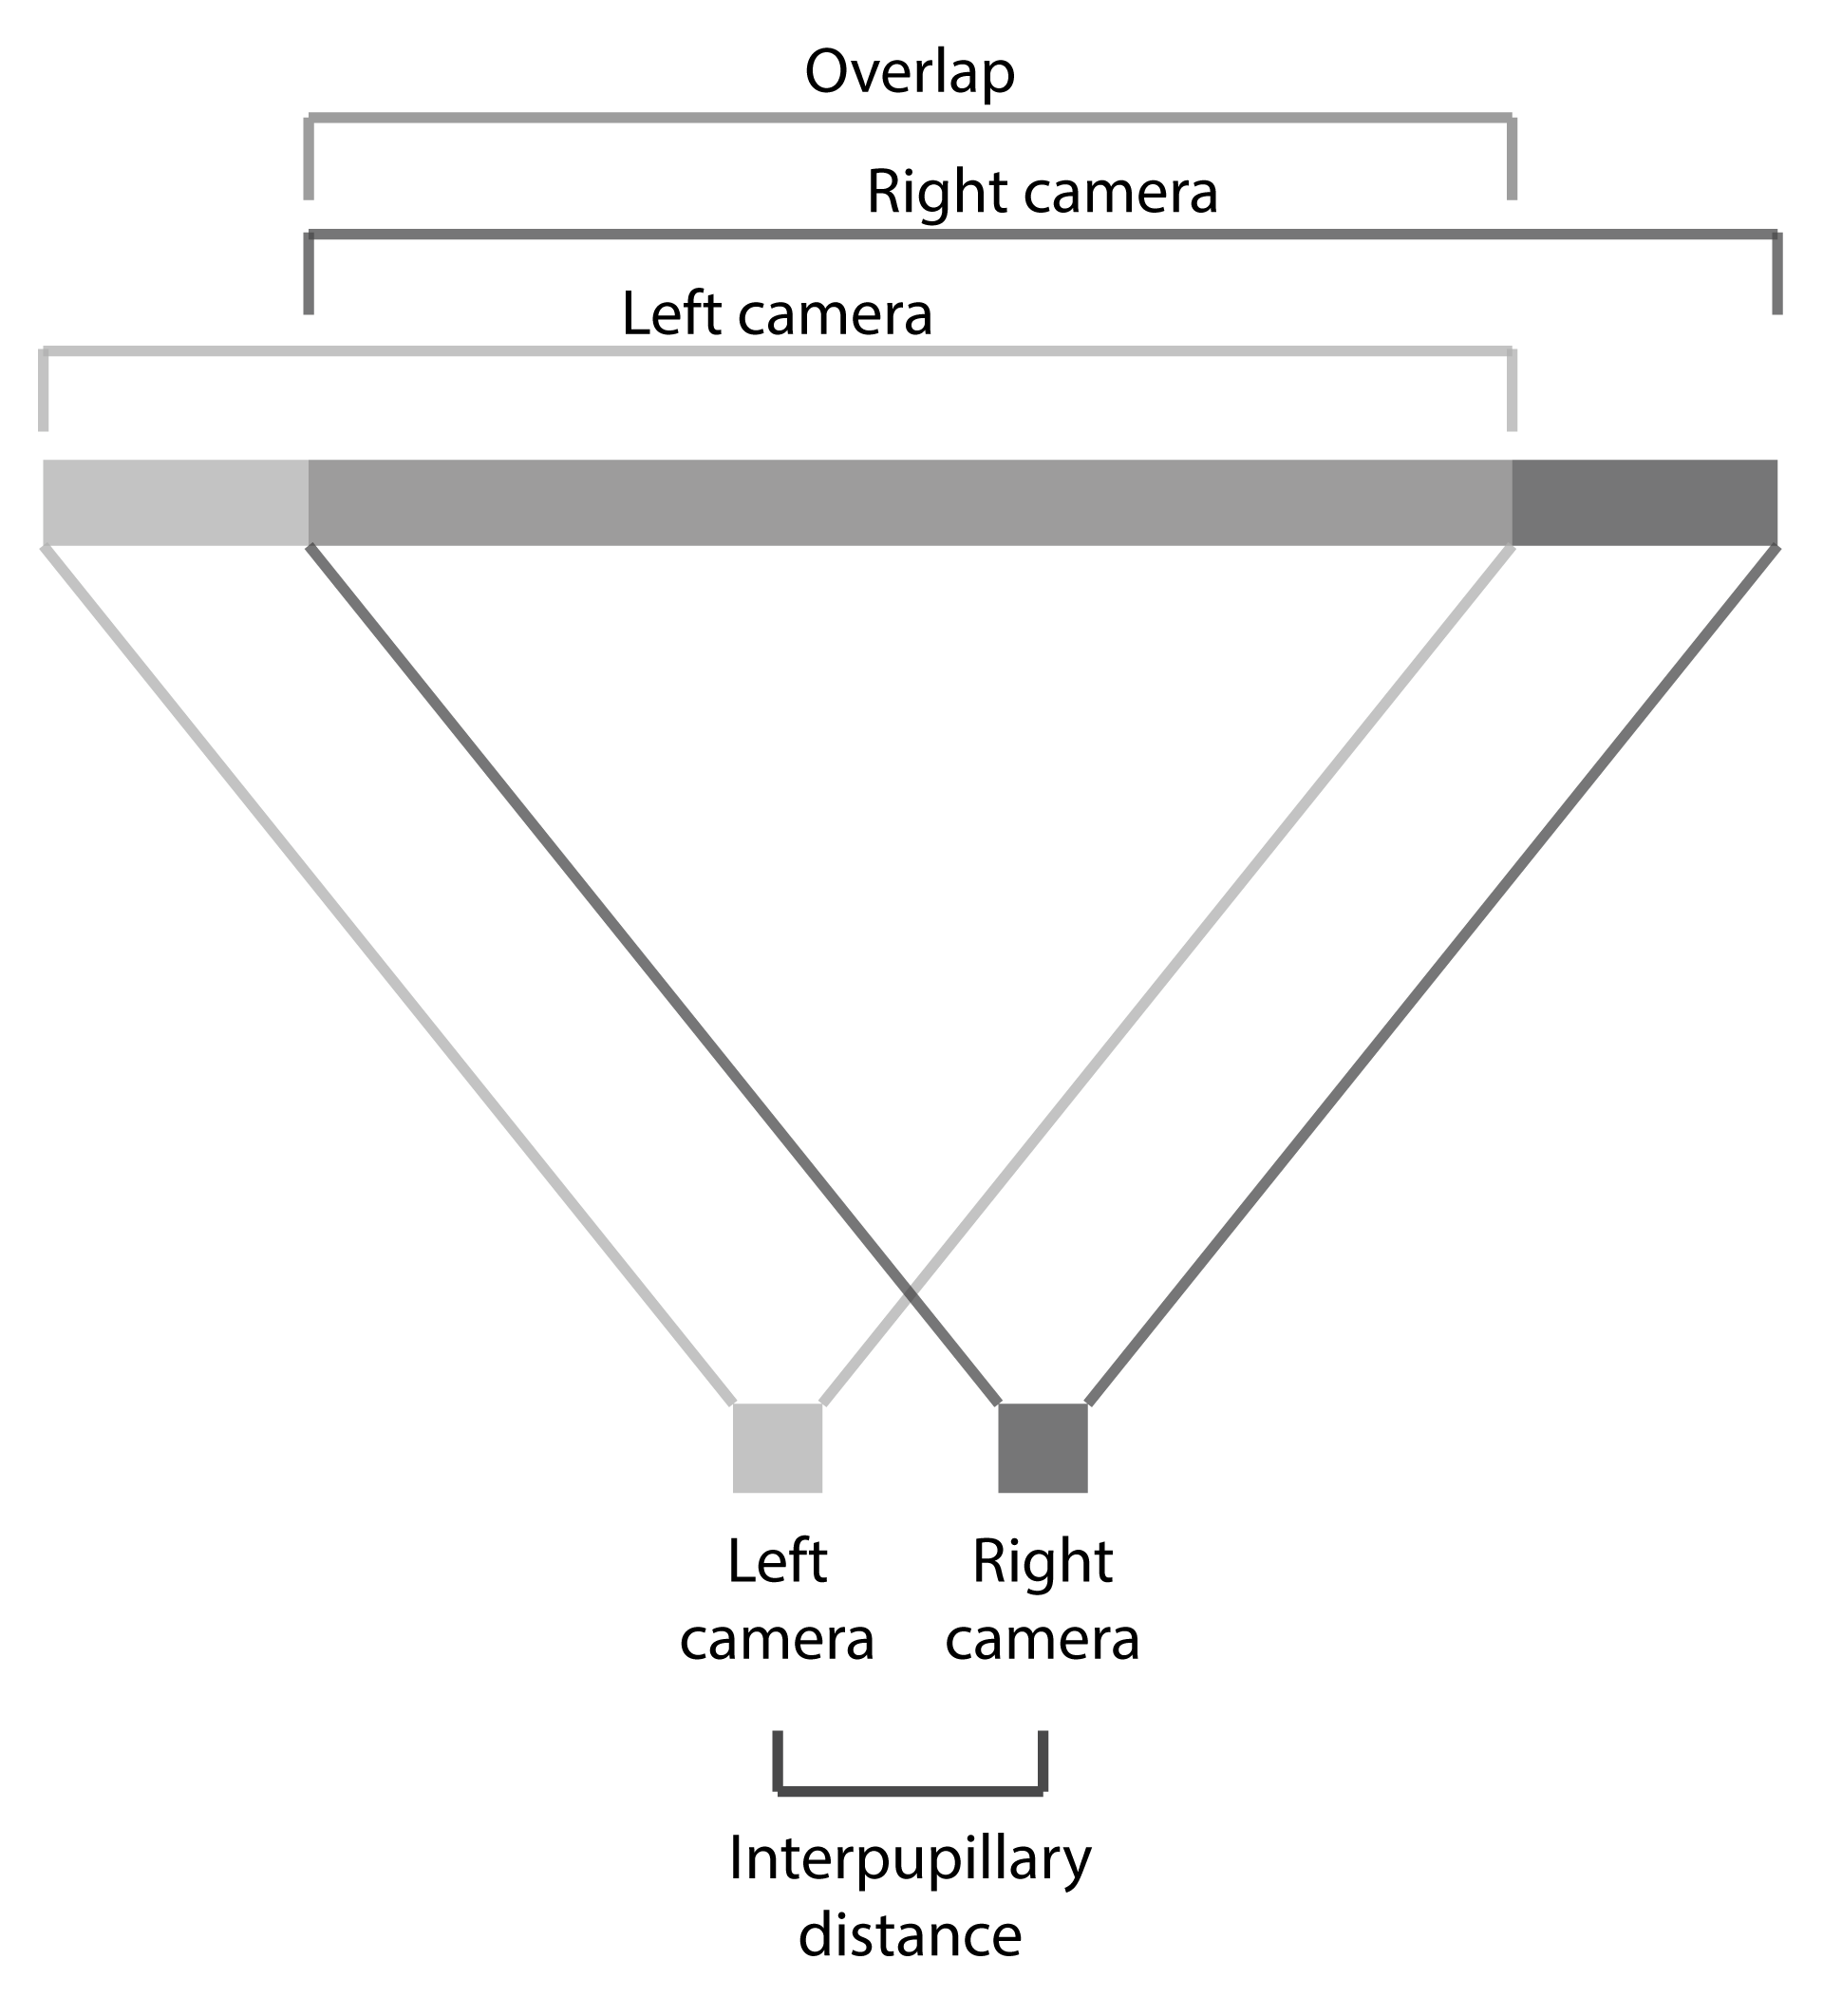
\includegraphics[width=.4\linewidth]{webcam-overlap.png}
		\caption{Visualisation of overlap between camera planes.}
		\label{webcam-overlap.png}
	\end{center}
\end{figure}

As the Mirrorshades platform needed to allow the user to control which environment they are perceiving, either real or virtual, the visibility of these camera planes (\& the virtual environment behind them) had to be controllable. The opacity of the camera planes was linked to the control mechanisms, however because the camera planes do not completely fill the DK1's FOV (see section \ref{modifying-dk1} and figure \ref{fov-comparison-1.png}) two further, larger planes were situated behind the camera planes to cover the entire FOV of the DK1. The opacity of these planes was also linked to the control mechanisms, such that when the user operates the control mechanism in a manner to view VR, they become completely transparent to allow VR visual stimuli to pass, but when the user operates the control mechanism in a manner to see RW, they become opaque to prevent any RW visual stimuli from passing around the camera planes. Even though these areas around the mediated camera streams are not strictly viewable, the ambient light that they would produce could be detrimental to the viewing of the RW camera streams.

The arrangement of these planes in relation to the virtual cameras is shown by figure \ref{unity-screenshot-6.png}, where it can be seen that the smaller camera planes do not fill the virtual cameras' frustum due to the narrower FOV of the C310 with 2.1mm lenses than of the DK1. Figure \ref{unity-screenshot-7.png} shows a space between the camera planes and the backing planes, required to avoid a rendering bug that arose with planes situated so close together.

\begin{figure}[h]
	\begin{center}
		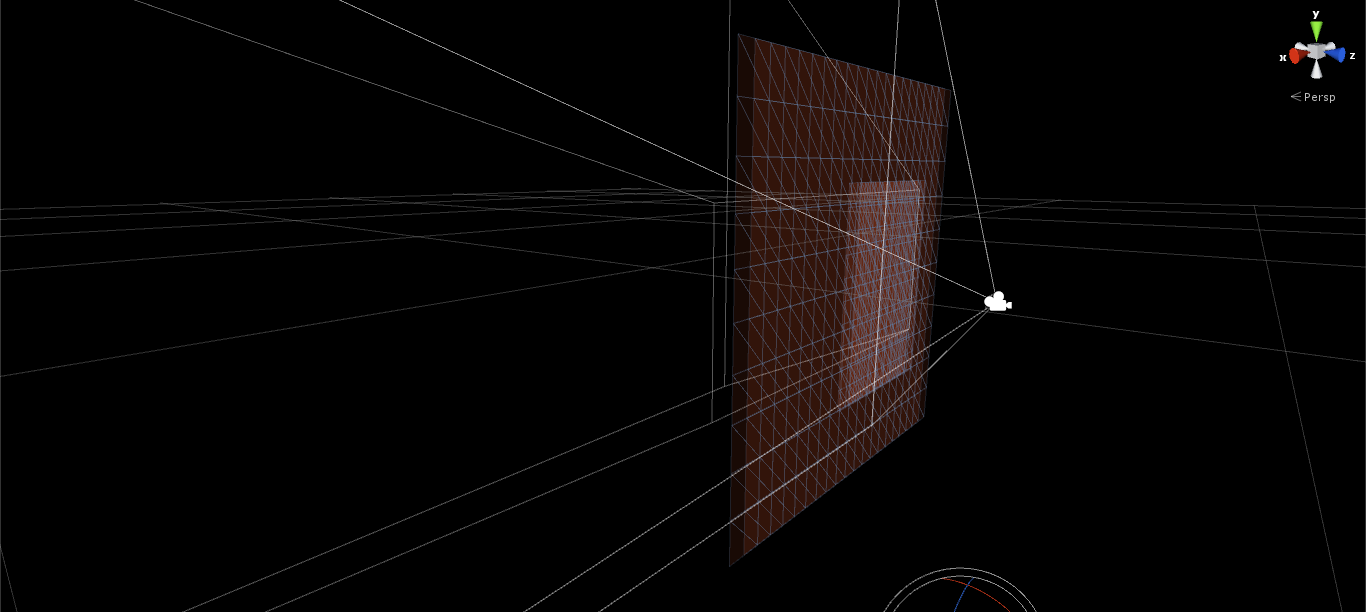
\includegraphics[width=.85\linewidth]{unity-screenshots/unity-screenshot-6.png}
		\caption{Arrangement of camera planes and backing planes in Unity.}
		\label{unity-screenshot-6.png}
	\end{center}
\end{figure}

\begin{figure}[h]
	\begin{center}
		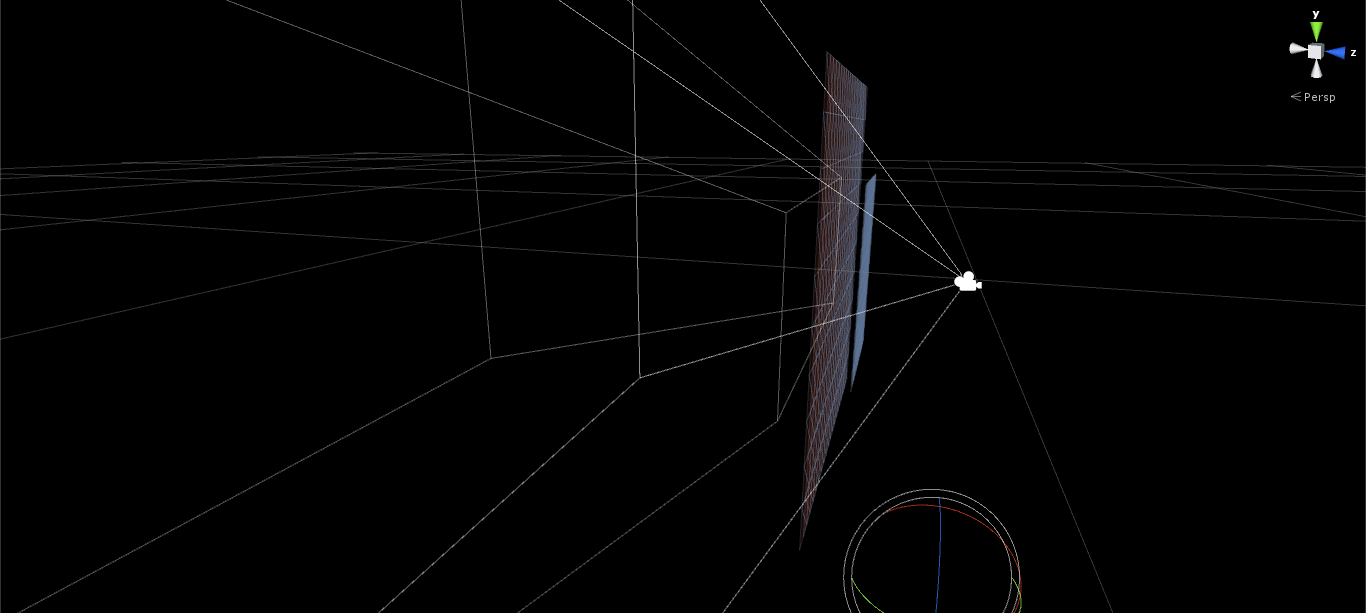
\includegraphics[width=.85\linewidth]{unity-screenshots/unity-screenshot-7.png}
		\caption{Spacing between camera planes and backing planes in Unity.}
		\label{unity-screenshot-7.png}
	\end{center}
\end{figure}

%=========================================================================================================

\subsection{Latency of DK1 Video See-Through Solution}

Measurement of the end-to-end latency of the C310 solution was performed by placing the DK1, with the lens cups removed, in front of a LCD monitor displaying a timer\footnote{\url{http://www.flatpanels.dk/monitortest_inputlag_dk.php}}. In this context end-to-end latency refers to the time taken for a visible change in the scene in front of the DK1 (such as the incrementing digits upon the monitor) to be reflected by a comparable change upon the DK1's display. This figure accounts for latency introduced by the C310 cameras themselves, by the Unity engine and by the DK1's display.

A digital camera was set up on a tripod behind the monitor and DK1 such that it could record both the monitor and the milliseconds value on the DK1's screen. The digital camera was set at a sufficiently high sensitivity as to record video at 50fps with a shutter speed of 1/4000 of a second. Both the monitor and the DK1's screen refreshed at 60Hz, each frame lasting for 16.67ms, whilst a 1/4000 of a second shutter on the camera meant that the exposure was made over 0.25ms. The response time of the monitor (quoted by the manufacturer as 8ms grey-to-grey) was evidently much higher than that of the Rift, as the tenths and even hundredths digit on the monitor was usually legible in each frame of the video whereas on the Rift the hundredths and thousandths digits were always illegible.

To determine an estimate of the latency of the DK1 and camera setup using Unity, adjacent video frames were identified where a transition from one tenth digit to the next was legible on the Rift's display and the hundredths/thousandths digits were legible on the monitor, such as the pair shown by figures \ref{vid1.jpg} and \ref{vid2.jpg}. From these values it can be inferred that the tenths digit on the DK1's screen (visible through the right eyecup hole) changed from 9 (figure \ref{vid1.jpg}) to 0 (figure \ref{vid2.jpg}) sometime between 181ms (figure \ref{vid1.jpg}) and 198ms (figure \ref{vid2.jpg}) on the monitor, which represents a latency of between 181ms and 198ms. Out of 11 pairs of frames like this identified, 7 pairs showed this 181-198ms latency, while 4 showed 198-215ms latency as seen in figures \ref{vid3.jpg} and \ref{vid4.jpg}.

\TwoFig{latency/vid1.jpg}{Measuring latency (video frame, 1/2).}{vid1.jpg}
       {latency/vid2.jpg}{Measuring latency (video frame, 2/2).}{vid2.jpg}

\TwoFig{latency/vid3.jpg}{Measuring latency (video frame, 1/2).}{vid3.jpg}
       {latency/vid4.jpg}{Measuring latency (video frame, 2/2).}{vid4.jpg}

\newpage

In addition to video frames still photographs taken at the same 1/4000 of a second shutter speed gave some more legible stills which corroborated this 181-251ms figure. This figure is substantially greater than the 30-60ms figure often quoted\footnote{\url{https://www.oculus.com/blog/the-latent-power-of-prediction/}} as the upper limit for an acceptable VR experience, however how much it affects a relatively slow style of interaction such as that of applying parallel reality to a cultural heritage site versus that of a fast application such as a competitive `twitch' gaming is open to interpretation from experimental evaluation.

\begin{figure}[h]
    \begin{center}
    \begin{minipage}{.32\textwidth}
        \begin{center}
        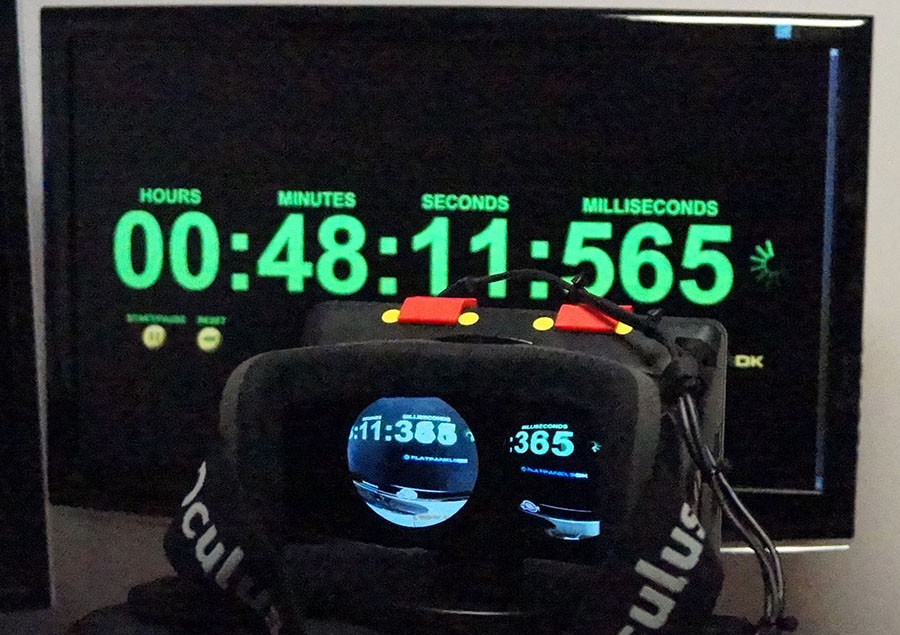
\includegraphics[width=\textwidth]{latency/still1.jpg}
        \caption{Measuring latency (still photograph, 1/3).}
        \label{still1.jpg}
        \end{center}
    \end{minipage}%
    \hspace{.01\textwidth}
    \begin{minipage}{.32\textwidth}
		\begin{center}
        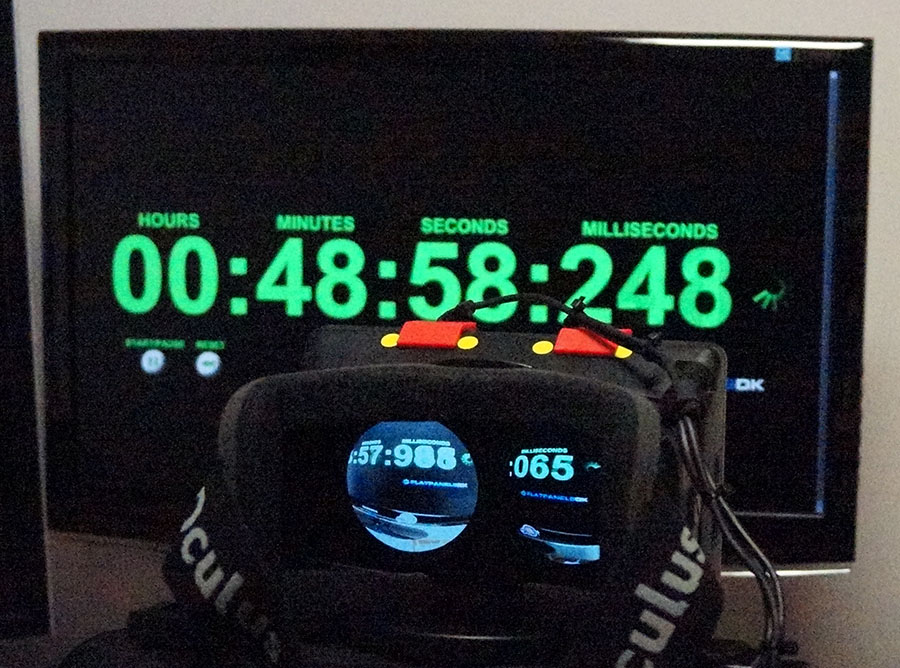
\includegraphics[width=\textwidth]{latency/still2.jpg}
        \caption{Measuring latency (still photograph, 2/3).}
        \label{still2.jpg}
        \end{center}
    \end{minipage}%
    \hspace{.01\textwidth}
    \begin{minipage}{.32\textwidth}
        \begin{center}
        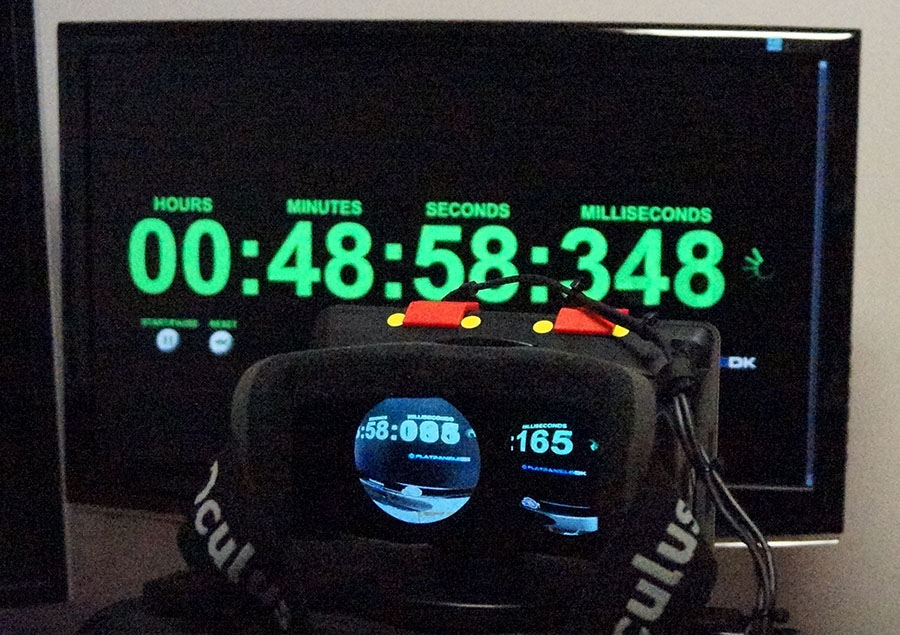
\includegraphics[width=\textwidth]{latency/still3.jpg}
        \caption{Measuring latency (still photograph, 3/3).}
        \label{still3.jpg}
        \end{center}
    \end{minipage}
    \end{center}
\end{figure}

%=========================================================================================================

\subsection{Constraints of DK1 Video See-Through Solution}

\label{constraints_of_dk1_see_through_solution}

Whilst the FOV of the image produced by the C310 is sufficient to fill the area of the DK1's screen visible when relief is extended to its furthest position, there are other aspects of the camera solution in addition to the latency that needed consideration, including the depth of field (DoF) of the images and their fixed convergence.

Due to the fact that depth of field of an image captured by a camera system increases both as lens focal length and sensor size decrease, the combination of a short focal length lens (such as the 2.1mm used in the DK1 solution) with a small sensor (such as the 1/4'' type used in the DK1 solution) results in a very large depth of field. The hyperfocal distance~\cite{Kingslake1992} of the DK1 solution is close enough to the user that the images have acceptable sharpness from roughly arm's length to infinity. It is only upon looking at something closer than this, such as paying close attention to a handheld controller, that the image loses acceptable sharpness, so the requirement for such interaction would need to be avoided where possible.

With regards to convergence, when viewing an object in the real world the eyes rotate such that the perpendicular axes that bisect each eye converge at the point that one is looking at. This results in disparity between the images produced by each eye, as each sees the object from a different angle due to the physical distance between the eyes. This disparity leads to stereopsis, which is one of the contributing factors that leads to our ability to perceive depth. Oculus exploit this situation with their HMDs, by presenting a slightly different image to each eye, allowing virtual objects to appear at varying distances behind or in front of the virtual display.

For a stereo camera solution however, the convergence between the cameras is fixed, unless one were to implement a complex system employing eye tracking to dynamically physically reorient the cameras to match the orientation of the eyes. Thus one can either chose to mount the cameras parallel to each other such that their optical axes never converge/converge at infinity, or to fix them `toed-in' such that they converge at a non infinite distance.

With parallel cameras, any object captured by the cameras at infinity will be cast to the surface of the virtual screen. However any object captured by the cameras closer than infinity will be cast in front of the virtual screen with negative parallax. Viewing an entire scene in this manner is uncomfortable and should be avoided. With toed-in cameras, objects beyond the convergence point will be rendered with positive parallax and will appear to be behind the virtual screen, whilst objects closer than the convergence point will be rendered with negative parallax and will appear to be in front of the virtual screen. This is much more comfortable than a parallel camera approach.

With toed-in cameras the distance of the convergence point from the user should be chosen to sit somewhere in the middle of the distances they will be observing for the particular environment and task. For Mirrorshades this distance was set to be somewhere in the region of 15 to 20ft, which results in the most comfortable and natural feeling experience when engaging in the behaviour of a visit to a cultural heritage site such as St Salvator's chapel, which involves observing aspects of the building and architecture predominantly within this range of distances.

Toed-in cameras lead to both depth plane curvature, which causes objects at the corners of the image to appear further away than those toward the centre, and keystone distortion, which causes vertical discrepancy between each image, as the cameras' sensors are oriented in different planes, such that for one camera an image will appear larger at one side than the other, whilst for the other camera the image will appear larger on the other side~\cite{Woods1993}. As with depth plane curvature, keystone distortion is worse toward the corners.

It should also be noted in this discussion that the DK1's combination of optics and rendering shader means that the user's eyes focus at infinity. This is intentional as focussing on a far away plane is less strenuous than focussing on one closer, especially one only a few inches from the eyes as is the case with the DK1's screen. However this has the effect that the user is focussing their eyes at infinity whilst perceiving objects at varying distances between them and infinity. This is a caveat inherent to the DK1 that cannot be avoided, however it should be noted that this is an additional degradation to the user's view of their RW environment whilst using the Mirrorshades platform which is not present when viewing the RW environment directly.

A further consideration is the discrepancy between the lateral position of the cameras' sensors and the users' eyes, caused by the fact that the cameras must be mounted to the front of the DK1 and thus several inches in front of the user's eyes. This has the effect of making the user experience viewing the real world from several inches in front of where their eyes truly are (as if their eyes were `on stalks'), whilst viewing VR or viewing RW without the DK1 does not suffer this effect. The distance between the sensors and the user's eyes was reduced when iterating from the first mounting mechanism with metal stand-offs (figure \ref{deep-mounts.jpg}) to the second mechanism with rubber washers (figure \ref{shallow-mounts.jpg}), however with the interaction style of Mirrorshades where the user is predominantly focussed on observing objects and architecture 15-20ft away the discrepancy was not expected to be noticeable - it would only be when trying to manipulate objects much closer to the eyes that the discrepancy would become prominent.

\TwoFig{rift-clips-cameras/deep-mounts.jpg}{Early camera mounts with large eye/sensor distance.}{deep-mounts.jpg}
       {rift-clips-cameras/shallow-mounts.jpg}{Later camera mounts with smaller eye/sensor distance.}{shallow-mounts.jpg}

%Because of the approach that the DK1 uses to produce a `3D' image, by using side-by-side stereoscopic rendering where each eye receives a different image, with these images horizontally separated on the single screen, the solution does not feature zero parallax.

%By displaying a different image to each eye, which are 

%This is however inherent to all side-by-side stereoscopic HMDs and is not a product of the modifications to the DK1 to afford it with video see through capabilities.

%(autostereoscopic displays feature zero parallax when the image is being formed on the monitor surface)

%=========================================================================================================

\subsection{Registration of Camera and Unity Visuals}
\label{registration-of-camera-and-unity-visuals}
As mentioned in section \ref{caseforpr} the registration between real and virtual objects in the Mirrorshades system is less critical than that of an augmented reality system, as virtual objects in parallel reality are seen as part of a complete VR environment rather than gaining context from their accurate superposition upon a background of the RW environment. Whilst accurate registration will intuitively have a positive effect upon user experience of the Mirrorshades platform, especially when interaction with a reduced maximum opacity of the RW visuals (see section \ref{subsub-baseopacity}) is considered, the context provided to virtual objects by their wider virtual background and an emphasis on an interaction style that switches between environments rather than permanently overlaying one upon the other means that highly accurate registration is less of a concern than for many applications of augmented reality. Registration accuracies insufficient for augmented reality experiences may well be sufficient for successful parallel reality experiences.

This lessened requirement for accurate registration allows the Mirrorshades platform to operate using just the DK1's head tracker without what Azuma refers to as \textit{``additional registration strategies''}~\cite{Azuma1997}. This tracker provides 1Khz sampling with roughly 2ms delay (from head movement to Unity receiving the data) and thanks to sensor fusion performed over data from the accelerometer, gyroscope and magnetometer, drift is reduced to negligible levels. Mitigating drift in the head tracking solution was important for Oculus as it is a requirement for any VR experience that has a fixed reference point such as \textit{``a game with a cockpit, where your head's orientation does not affect the position of whatever car/plane/mech you're piloting''}\footnote{\url{https://www.kickstarter.com/projects/1523379957/oculus-rift-step-into-the-game/posts/380099}}\saveFN\rifttrackerfn. It would result in a poor VR experience if drift was allowed to mount between a user's head orientation and this fixed reference point: \textit{``imagine re-orienting your head back to perfect center but in-game you're now looking slightly left or right''}\useFN\rifttrackerfn .

In the case of Mirrorshades the fixed reference point is the chapel - both the RW and the VR chapel, as they occupy the same `place'. By making sure that the two chapels are aligned at the beginning of each session, the negligible drift in the head tracker means that sufficient registration between the two environments is maintained throughout the experience without the need to introduce any additional registration strategies. This alignment is achieved by knowing the starting orientation of the virtual cameras in the VR chapel and then physically placing the DK1 in the corresponding orientation in the RW chapel. This starting orientation in the VR chapel is shown in figure \ref{sallies-rift-frame-of-reference.png} and producing the same orientation with the DK1 is trivial as it was chosen to be parallel with the architecture of the building (including the floor tiles, which proved to be a useful grid to accurately align the DK1 against).

\begin{figure}
	\begin{center}
		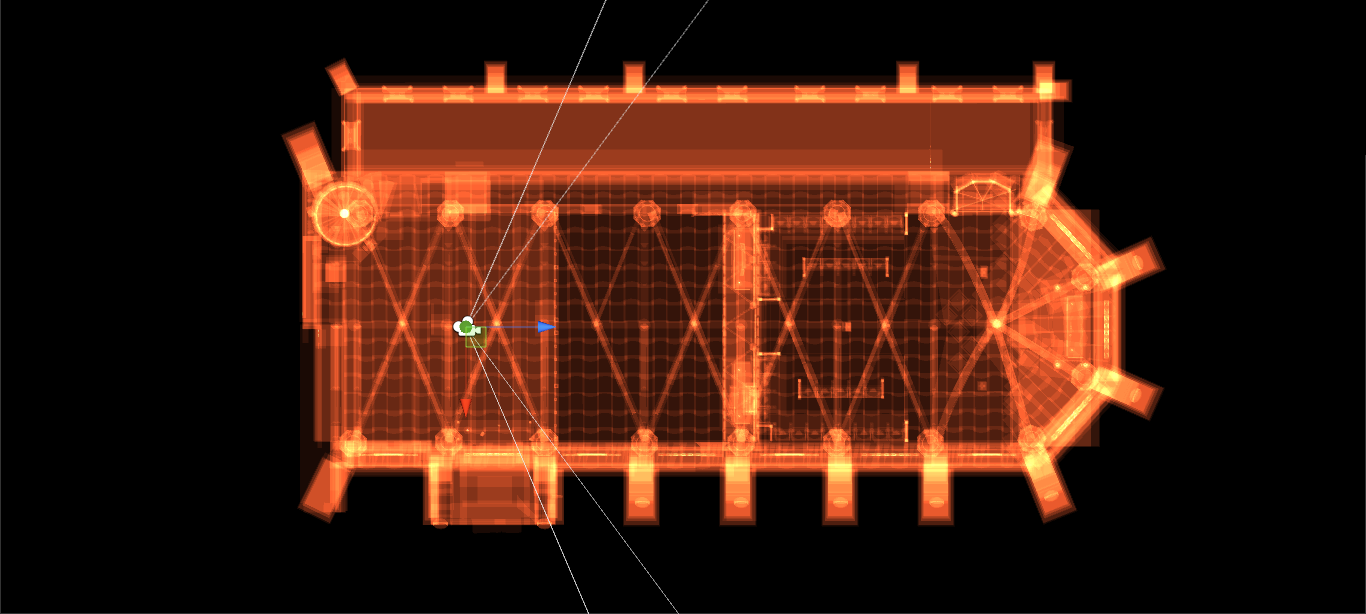
\includegraphics[width=.85\linewidth]{sallies-rift-frame-of-reference.png}
		\caption{Top down view of starting orientation of virtual cameras (toward left side and facing the right, frustum lines visible in white) within Unity chapel reconstruction.}
		\label{sallies-rift-frame-of-reference.png}
	\end{center}
\end{figure}

%=========================================================================================================

\section{Indoor Positioning System}

For outdoor applications GPS represents a suitable solution for the vast majority of position tracking requirements. Global coverage and the ability to scale accuracy as required, from many metres with a basic GPS receiver such as those integrated into smartphones, to a few metres with SBAS augmentations and further to as little as 10cm with the (costly) deployment of Differential GPS (DGPS) beacons, has led to GPS occupying the role of the `go to' solution where position tracking is required for an outdoor application. For indoor applications however there is no single technology or solution that provides such encompassing suitability as GPS does outdoors and as such a large number of different technologies have been employed to produce IPS, which are summarised in table \ref{mautz-table.png}.

\begin{table}[h]
	\begin{center}
		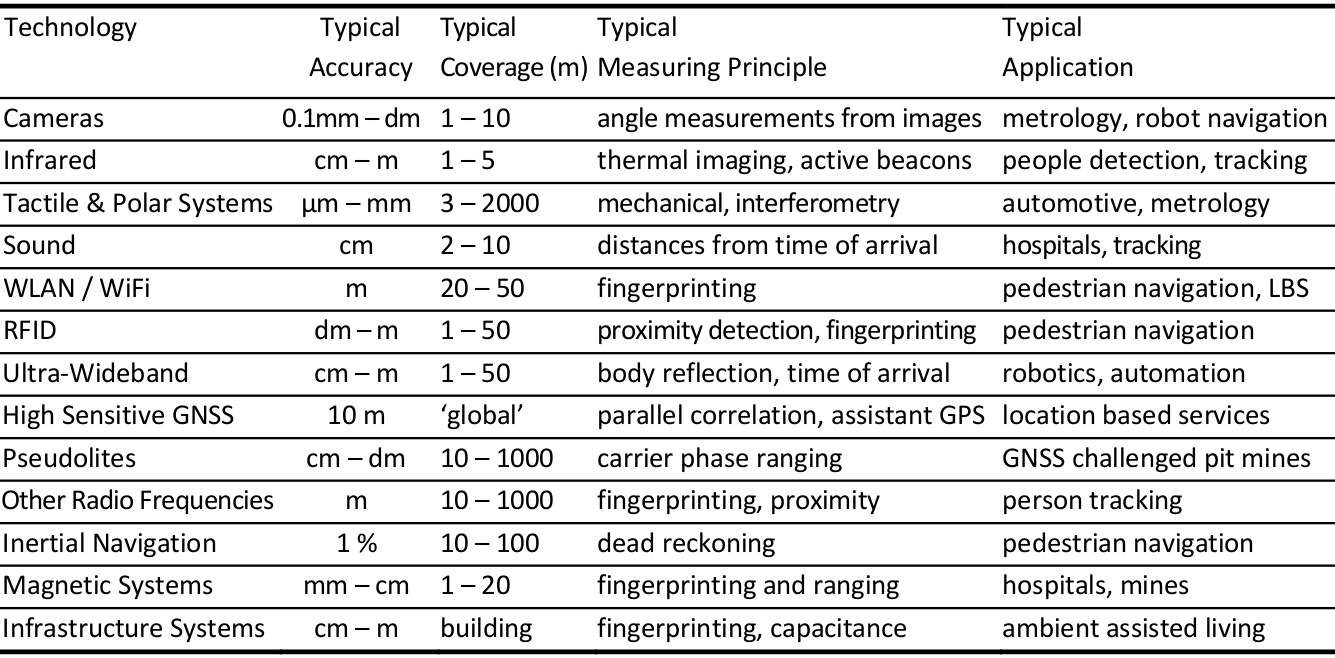
\includegraphics[width=\linewidth]{mautz-table.png}
	\end{center}
	\caption{Overview of IPS technologies, table courtesy Rainer Mautz~\cite{Mautz2012}.}
	\label{mautz-table.png}
\end{table}

Because of this diversity in technologies, with different IPS solutions covering various swathes of the continuums of accuracy and coverage (see figure \ref{Mautz-000.png}) and introducing a host of performance and suitability considerations, it is necessary to carefully consider the requirements of an indoor positioning application (see figure \ref{Mautz-003.png}) in order to choose the best suited of the many different IPS approaches. Unsurprisingly selection of one approach usually leads to balancing these requirements in a trade-off, as each of the challenges of indoor positioning can effect each technology differently~\cite{Mautz2009}.

\TwoFig{Mautz-000.png}{IPS technologies plotted against their accuracy and coverage, image courtesy Rainer Mautz~\cite{Mautz2012}.}{Mautz-000.png}
       {Mautz-003.png}{Requirements parameters of IPS, image courtesy Rainer Mautz~\cite{Mautz2012}.}{Mautz-003.png}

%=========================================================================================================

\subsection{IPS Requirements for Mirrorshades}
\label{ips-requirements-for-mirrorshades}
In order to fully investigate the freeform exploration scenario and aspects of the detailed comparison scenario described in section \ref{parallel-reality-in-virtual-heritage}, the Mirrorshades platform needed to employ more accurate position tracking than the GPS solution used by VTW. As a pedestrian application wherein the user walks through doorways (whether real or virtual) and observes multiple rooms within a building, it was necessary to achieve a level of accuracy that allowed for reliable distinction between adjacent rooms, between doorways and their surrounding walls and to approximate position within rooms and corridors.

Coverage required depended largely upon the size of the cultural heritage site that Mirrorshades was to be deployed to, however it seemed prudent to adopt an IPS that could scale as arbitrarily as possible from small scenarios (perhaps of a small village church) to larger scenarios (such as a cathedral) such that the suitability of the platform wasn't restricted to sites of particular sizes.

A high update frequency was not considered especially important for Mirrorshades. The style of interaction for either the freeform scenario or the freeform scenario with detailed comparison is one wherein users walk relatively slowly through the environments, as they wish to observe and take in their surroundings. Updates in the range of several hz was thought to be sufficient, especially if users were attending more to their real environment than the equivalent virtual environment when actively moving around (which was to be encouraged, as one cannot walk through an unattended RW obstacle as one can a VR one). Similarly, low latency was not considered to be critical. Even if the IPS took a few seconds to `catch up' with the user, if they are committed to a deliberate study and comparison of their real and virtual surroundings they would not be foiled in this task if they found that they had to wait momentarily when switching from real to virtual views.

Cost represented a more concrete restriction for Mirrorshades, as the costs of installing and using different IPS range drastically. For example, an IPS that locates users via propagation modelling/empirical fingerprinting/pathloss of WiFi signals can make use of existing WiFi infrastructure installed in a building and use nothing more expensive than a smartphone carried by the mobile user, however this does not provide especially accurate readings. At the other end of the cost spectrum, using a motion capture suit as an IPS solution incurs substantial costs for each suit, with additional costs for the supporting infrastructure, although provides extremely high accuracy. In a project similar to Simeone et al.'s substitutional reality (see section \ref{spatial-equivalence}) the Oculus Rift HMD was combined with an Xsens MVN motion capture suit, allowing participants to walk around a virtual environment of the same layout and dimensions as their real environment, but without any video see-through of that real environment\footnote{\url{https://www.youtube.com/watch?v=LtMfrkRqlRs}}. The use of a motion capture suit allowed extremely accurate positional tracking, however as a \textit{``complete standard Xsens MVN system is available at around \euro{}50,000''}\footnote{Personal correspondence with Xsens EMEA Entertainment Business Manager.} and requires a not insubstantial setup phase of the participant donning the suit, it is unsuitable for a virtual heritage scenario wherein budget is likely to be substantially more limited and  where visitors are unlikely to be willing to don a complex motion capture suit in order to explore the site. To illustrate a real world comparison of the trade off between costs, accuracy, frequency, etc. considering the department building shown by figure \ref{jack-cole-splodges-red.png} \textit{``To cover ground floor and have room level accuracy in each room + tracking in the corridors, the cost would be ca. \$25,000''}\footnote{Personal correspondence with Sonitor Technologies Vice President Sales and Business Development EMEA and APAC.} for a commercial ultrasonic solution.

Reliance upon deployed infrastructure such as beacons and markers also needed to be avoided for a parallel reality platforms within virtual heritage, as most cultural heritage sites would not take kindly to the installation of any such infrastructure into the site/environment, or may only have allowed strictly temporary infrastructure to be deployed. Approaches that required extensive infrastructure to be deployed, or for which the deployment and calibration phase of infrastructure is time consuming, were therefore unsuitable. Similarly, intrusiveness of the IPS used for parallel reality platforms in virtual heritage needed to be considered such that the IPS did not too negatively affect the user's experience of the real and virtual sites around them, in a situation where immersion is a primary goal.

Robustness of all aspects of a virtual heritage system are critical for enjoyment and beneficial experience by the user. Visitors to a cultural heritage site, especially if they are only visiting for a short period of time, are not pliant to waiting for a malfunctioning virtual heritage system to right itself. Furthermore, many virtual heritage systems are installed by experts into locations where the permanent on-site staff do not have the technical knowledge or experience to troubleshoot and repair them, so these systems must be robust enough to continue successful operation for extended periods of time without intervention and maintenance by knowledgeable support staff.

%http://www.memsic.com/wireless-sensor-networks/MCS-KIT410CA
%8x Crickets
%GBP1850
%email from Willow.co.uk

%=========================================================================================================

\subsection{PlayStation Move}
\label{psmove}
One technology investigated for suitability as an IPS for use with Mirrorshades was PlayStation Move (PSMove), a game controller platform released by Sony for use with their PlayStation 3 console. The PSMove tracks a hand held controller which contains inertial sensors and has a plastic sphere on its end that is illuminated from within by a RGB LED, using the bundled PS3 Eye camera to track the controller's position in relation to itself. Through use of the PSMove API~\cite{Perl2012} the PSMove platform can be used by a regular computer, making use of the OpenCV\footnote{\url{http://opencv.org/}} computer vision project.

Whilst PSMove has been used successfully for pedestrian position tracking in previous projects, including at least one that used an Oculus Rift HMD\footnote{\url{http://projects.ict.usc.edu/mxr/blog/project-holodeck-wows-in-dublin/}}, it quickly became apparent when auditioning the platform that it only performs reliably in dimly lit conditions. Even the relatively dim scene shown by figure \ref{psmove-screenshot.png} represented too much ambient light for reliable tracking, so the suitability of the platform for use at a cultural heritage site where illumination is unlikely to be controllable was negated.

\begin{figure}[h]
	\begin{center}
		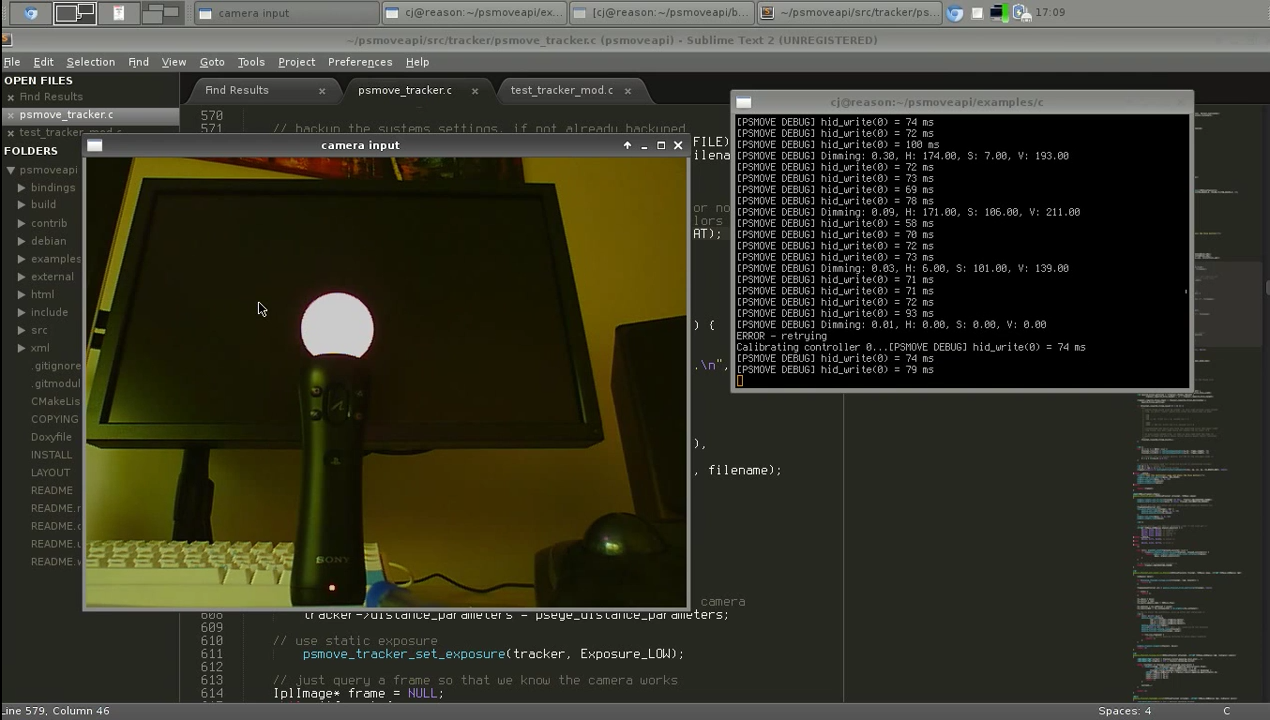
\includegraphics[width=.8\linewidth]{psmove-screenshot.png}
		\caption{PSMove failing to locate illuminated marker even in relatively dim conditions.}
		\label{psmove-screenshot.png}
	\end{center}
\end{figure}

%=========================================================================================================

\subsection{Indoor Atlas}

During the evaluation phase of different IPS and their suitability to the Mirrorshades platform and its application to St Salvator's chapel, Finnish startup IndoorAtlas\footnote{\url{https://www.indooratlas.com/}} released the first public beta of their indoor positioning technology that uses the magnetometers found in smartphones to locate a user within a magnetic `fingerprint' of a building. This approach takes inspiration from animals such as the spiny lobster that are able to determine their position from the Earth's magnetic field~\cite{Boles2003}. A spin out from research at the University of Oulu in 2009~\cite{Haverinen2009,Haverinen2009a}, with a similar project undertaken by Media Lab researchers in 2011~\cite{Chung2011}, IndoorAtlas exploits how the Earth's magnetic field is distorted by both natural and man-made sources - distortions that VTW had to \textit{contend} with to produce accurate compass bearings. Indoors these distortions come from building materials, especially in modern structures employing a framework of metal beams, but also from electrical cabling, HVAC ducting, concrete rebar, etc. By recording a map of these distortions in an offline mapping phase, producing a fingerpint of the magnetic field around a building, the location of a user can be deduced by comparing the readings from their smartphone's magnetometer to this fingerprint.

IndoorAtlas represented a good match for the IPS requirements of the Mirrorshades platform. In particular the lack of dependence upon any deployed infrastructure such as ultrasound beacons or visual tracking targets suited the deployment area of Mirrorshades well, as most cultural heritage sites would not be amenable to the deployment of such hardware. Furthermore the reliance upon only a smartphone held by the user meant that coverage would only be limited by the area that had been mapped in the offline mapping phase, allowing the positioning to scale to arbitrarily large indoor cultural heritage sites. This requirement for only a smartphone also met the low cost requirement of the Mirrorshades platform, as mid to high end smartphones with sensitive magnetometers can presently be purchased for just a few hundred dollars.

The major concern at this point was whether the building materials employed in the construction of cultural heritage sites such as chapels, castles and cathedrals would create large enough distortions to the Earth's magnetic field for IndoorAtlas to provide its boasted accuracy. This accuracy would be sufficient to discern between adjacent rooms, between doorways and their surrounding walls and to estimate user position within rooms and corridors. The building materials of the sites are largely various types of stone and wood, a far cry from the metal framework that permeates most modern buildings. Whilst initial tests of the IndoorAtlas beta technology within a department building of roughly 40m across (videos of which are available to view online\footnote{\url{https://www.youtube.com/watch?v=l-eIvzpScRs}}\footnote{\url{https://www.youtube.com/watch?v=9hc2zEeQJXQ}}) were promising, this was a modern building with a steel beam structure and an abundance of computing infrastructure and its associated cabling and cooling provision (see figure \ref{jack-cole-ceiling.jpg}). Figure \ref{jack-cole-splodges-red.png} shows the results of one of these tests, with each red dot representing a position reported by IndoorAtlas while walking around the building at a slow walking pace ($<1$ms$^{-1}$, akin to the speed that visitors to cultural heritage sites tend to adopt).

\begin{figure}[h]
	\begin{center}
		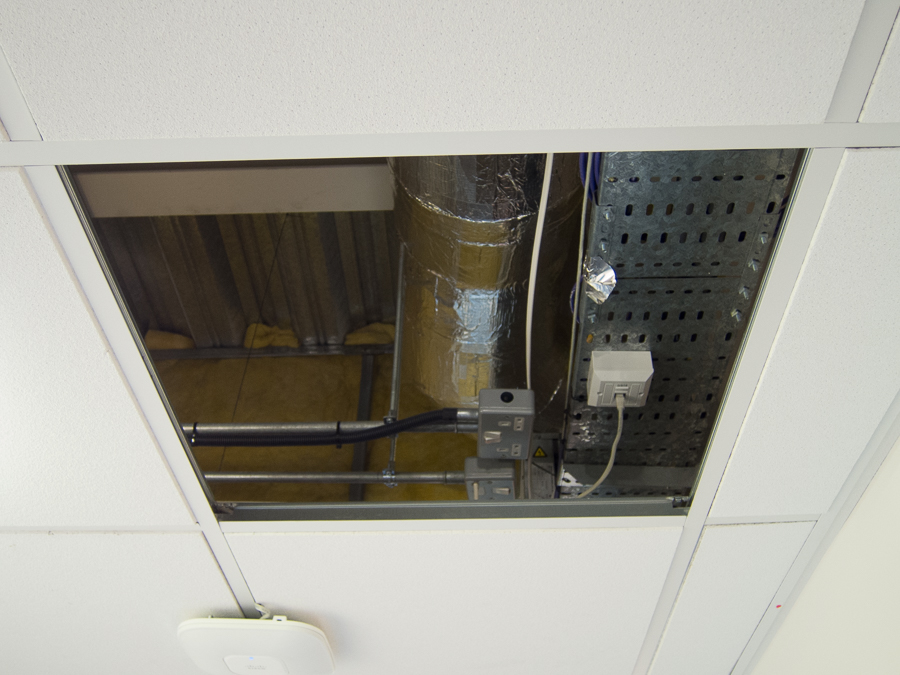
\includegraphics[width=.6\linewidth]{jack-cole-ceiling.jpg}
		\caption{Metalwork abundant in department building ceiling.}
		\label{jack-cole-ceiling.jpg}
	\end{center}
\end{figure}

\TwoFig{jack-cole-splodges-red.png}{Positions reported by IndoorAtlas within department building.}{jack-cole-splodges-red.png}
       {jack-cole-indooratlas-routes.png}{Route mapped in department building during offline mapping phase.}{jack-cole-indooratlas-routes.png}

It should be noted that the IndoorAtlas technology only reports positions upon routes that have been previously mapped in the offline mapping phase. For the positions shown in figure \ref{jack-cole-splodges-red.png}, this offline mapping phase mapped the route shown by the thick black line in figure \ref{jack-cole-indooratlas-routes.png}. In the subsequent test, had the user deviated from this route, IndoorAtlas would still have reported them as being somewhere upon it; it would not have attempted to extrapolate their position into unmapped territory. This is presumably because the scale of distortions in the Earth's magnetic field is quite fine grained, which is supported by the fact that many of the red dots are less than a meter apart, thus extrapolation would not fair well. This was an important aspect to take into account when performing the offline mapping phase of the chapel, as one must map sufficient paths to cover all possible places and routes that a user may walk. For locations comprised mainly of corridors and small rooms, this issue is trivial, however for a location that contains any large open space in which the user is free to meander, a more involved mapping process is required in which the entire space is systematically covered by back and forth routes that progress across the space. One substantial benefit of this situation is that inaccuracies in the IPS will never cause the user's position to be reported at `impossible' locations such as inside of walls, whereas inaccuracies with GPS data can result in the user's position being reported at such locations. 

Initial testing of IndoorAtlas at St Salvator's chapel proved surprisingly successful, with the platform able to track the smartphone accurately throughout the building even without any obvious overbearing metal content in the structure or its furnishings. Figure \ref{sallies-splodges-red.png} shows the set of positions reported by the IndoorAtlas platform whilst walking throughout the chapel, which is roughly 30m across, after an offline mapping phase that mapped the routes shown in figure \ref{sallies-indoor-atlas-routes.png}. The nave area on the left of the floorplan images, which appears fairly clear, is in fact populated in the real world by rows of chairs, thus the requirement for only the two crossing paths to be mapped therein.

\TwoFig{sallies-splodges-red.png}{Positions reported during preliminary testing of IndoorAtlas at St Salvator's chapel.}{sallies-splodges-red.png}
       {sallies-indoor-atlas-routes.png}{Routes mapped in St Salvator's chapel during offline mapping phase.}{sallies-indoor-atlas-routes.png}

Upon closer inspection of the chapel, metal gratings set into the floor and which run along the central aisle, representing much of the horizontal movement in figure \ref{sallies-splodges-red.png} and shown in figure \ref{DSCN0172.jpg} and figure \ref{DSCN0174.jpg} in detail, may explain this unexpectedly high performance. These gratings also extend to the open area in front of the altar as shown in figure \ref{DSCN0175.jpg}, however in other areas such as when walking to either side of the altar (far right of figures \ref{sallies-splodges-red.png} and \ref{sallies-indoor-atlas-routes.png}) there were no such obvious sources of magnetic interference (see figure \ref{DSCN0176.jpg}) to account for the maintained accuracy. Less obvious explanations could be possible ferromagnetic properties of the stone used in the building's construction and the presence of electrical lighting and audio systems (loudspeaker and light fixture visible in figure \ref{DSCN0177.jpg}) which presumably make use of electrical cables routed throughout the building.

\begin{figure}[h]
    \begin{center}
    \begin{minipage}{.32\textwidth}
        \begin{center}
        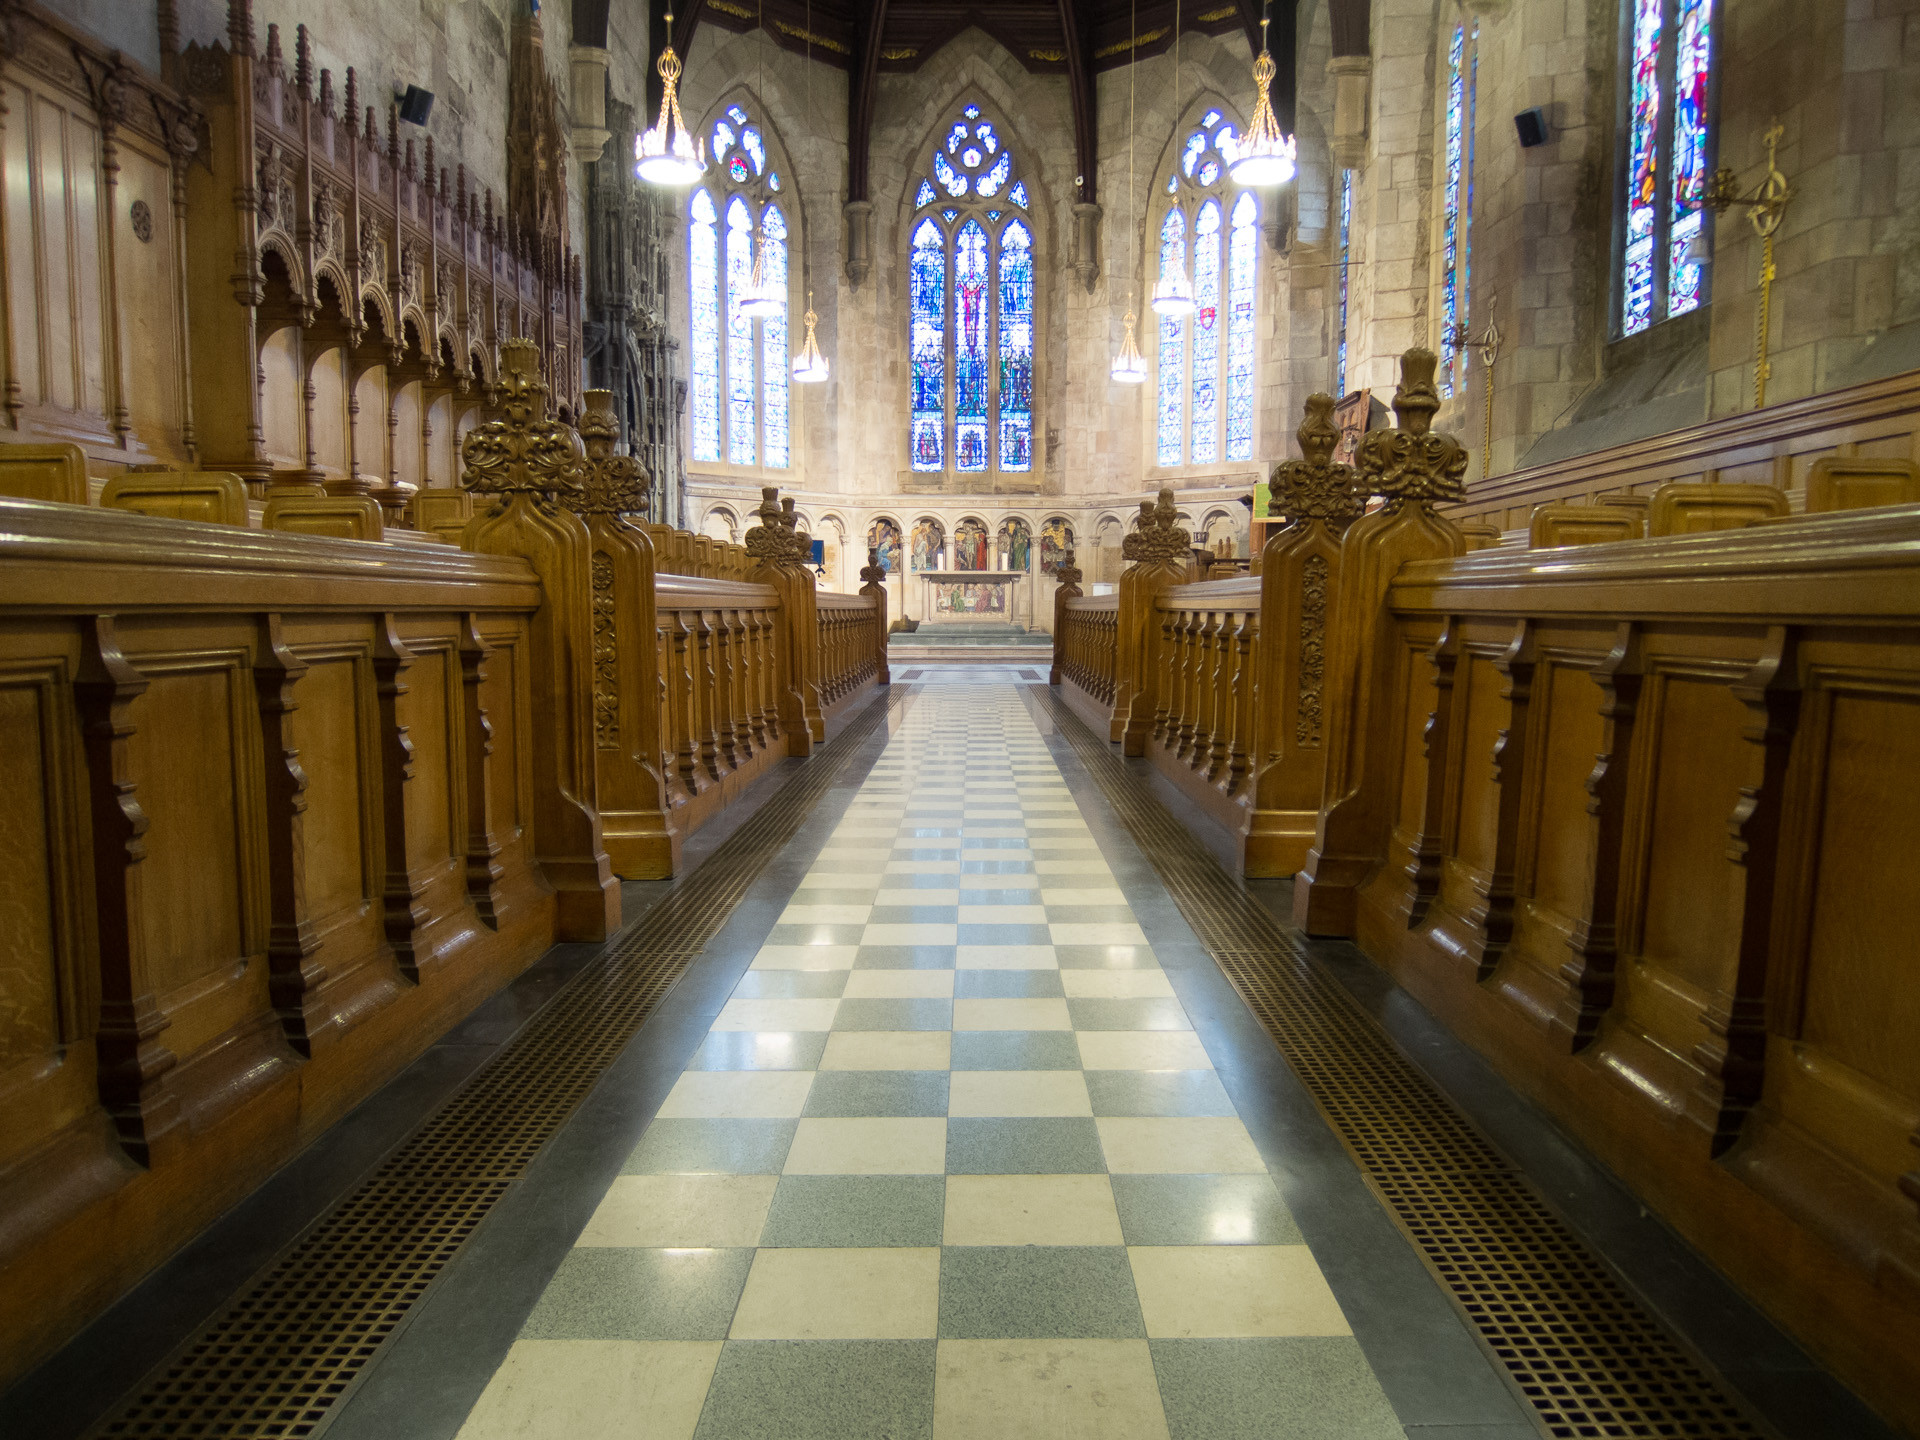
\includegraphics[width=\textwidth]{Sallies-photos/DSCN0172.jpg}
        \caption{St Salvator's chapel aisle, flanked by metal gratings.}
        \label{DSCN0172.jpg}
        \end{center}
    \end{minipage}%
    \hspace{.01\textwidth}
    \begin{minipage}{.32\textwidth}
		\begin{center}
        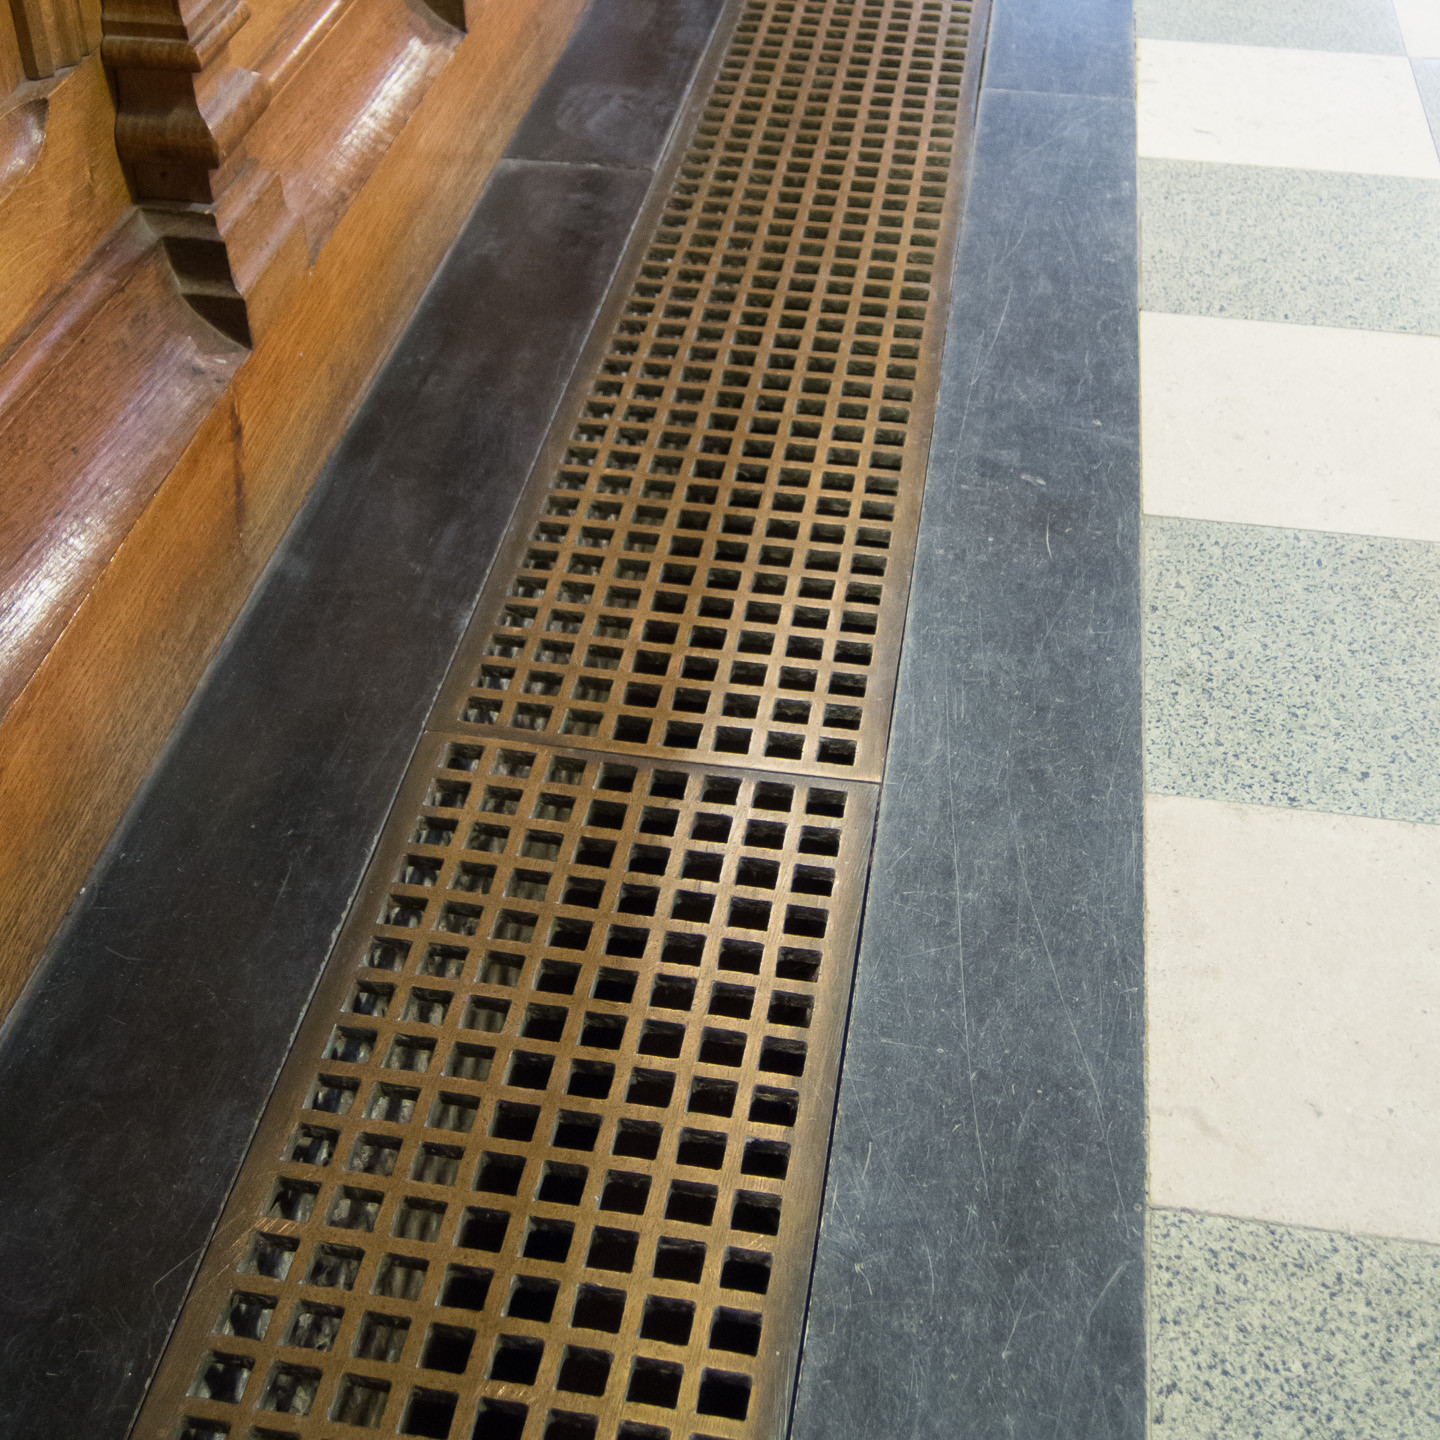
\includegraphics[width=\textwidth]{Sallies-photos/DSCN0174.jpg}
        \caption{Detail of St Salvator's chapel metal gratings.}
        \label{DSCN0174.jpg}
        \end{center}
    \end{minipage}%
    \hspace{.01\textwidth}
    \begin{minipage}{.32\textwidth}
        \begin{center}
        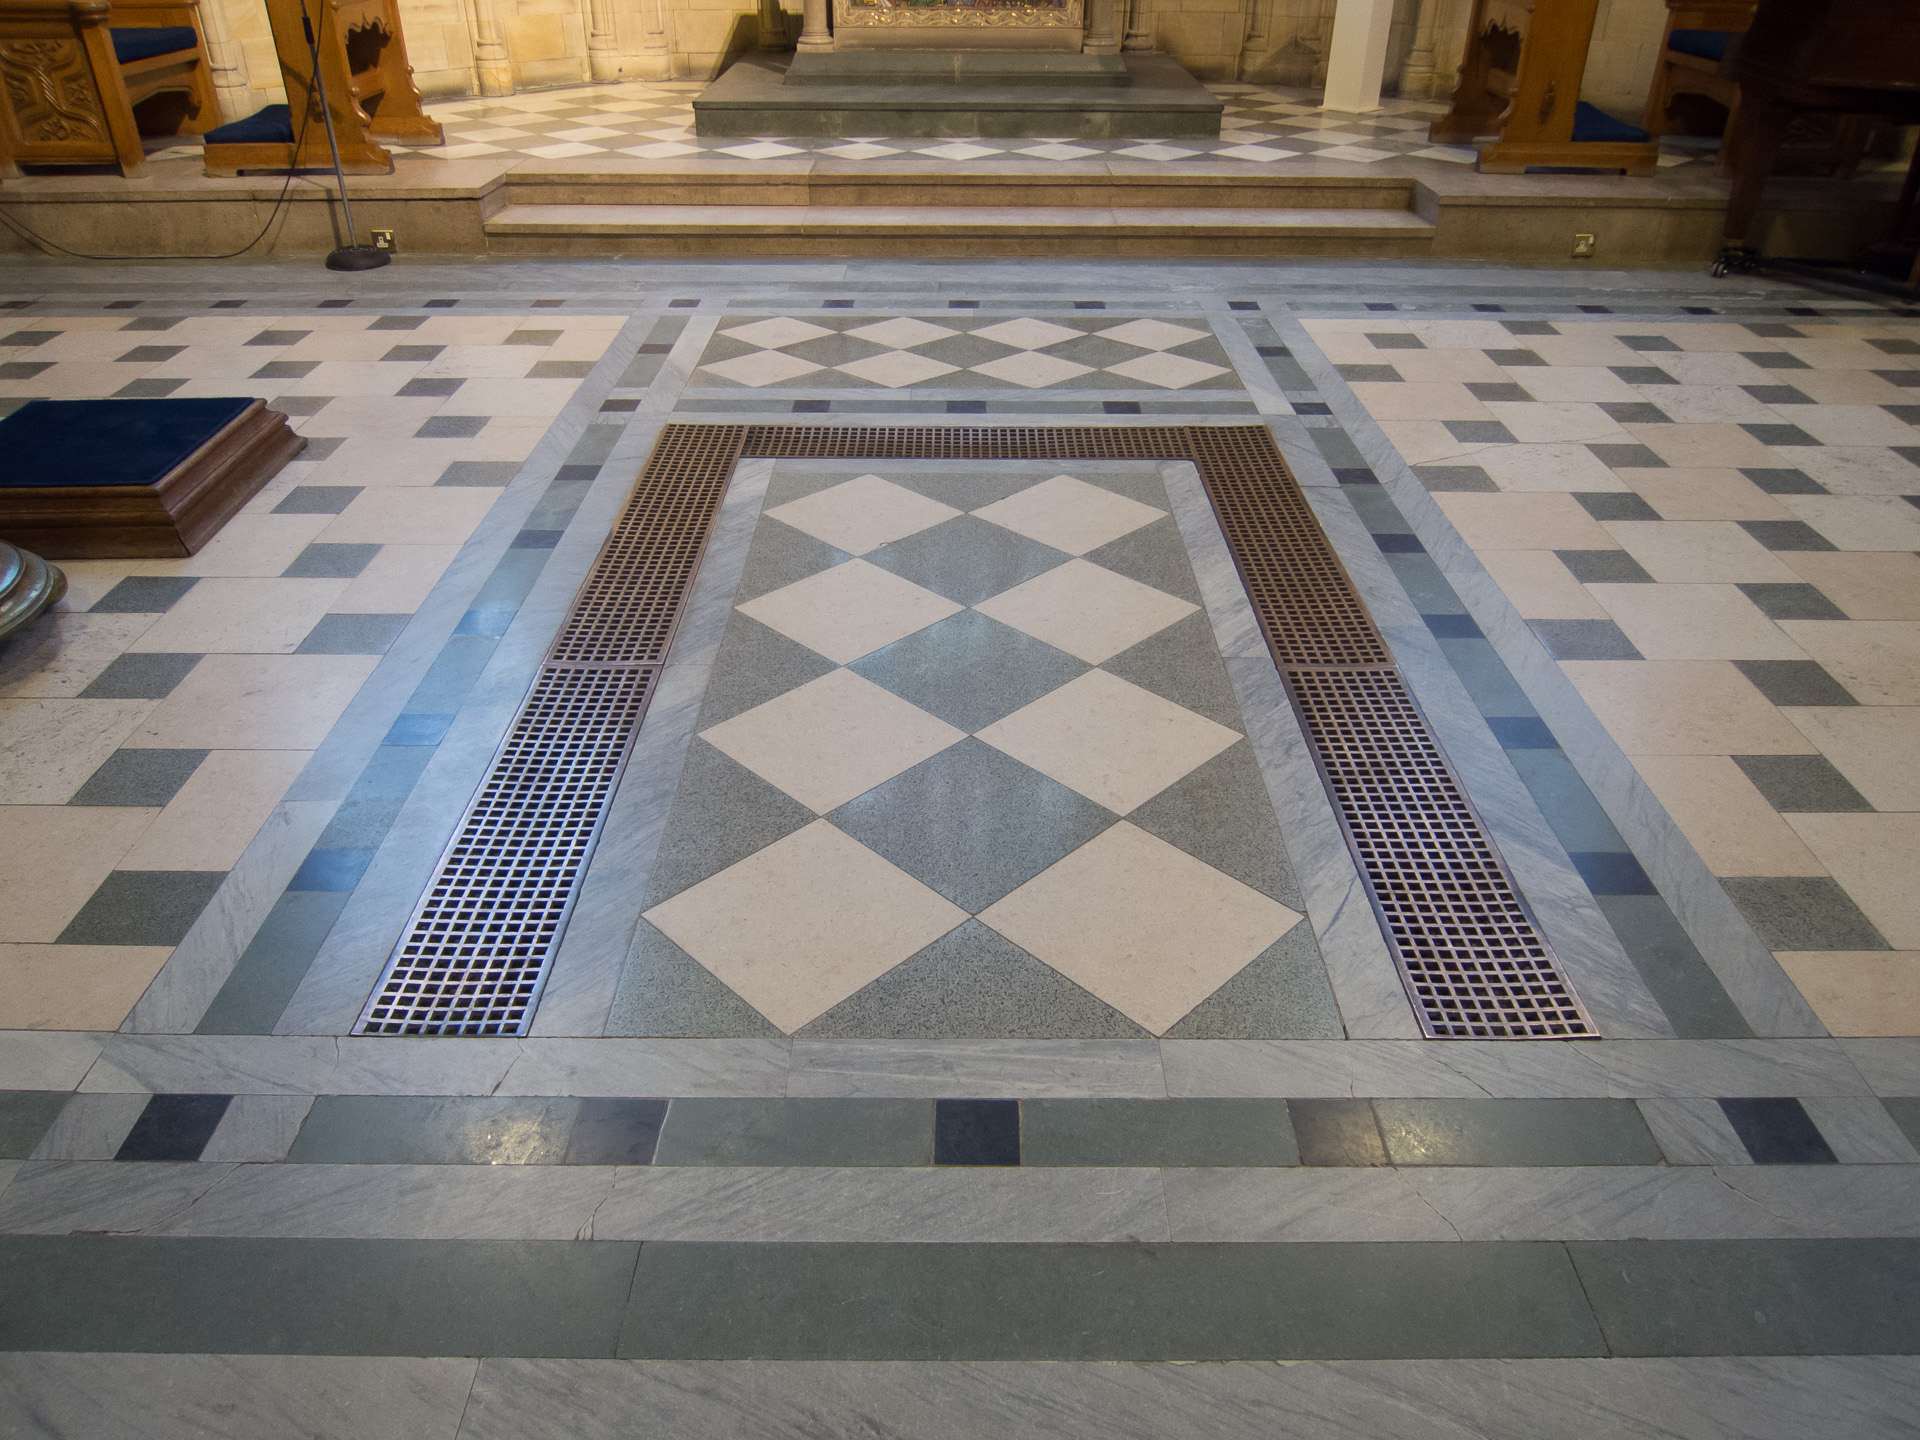
\includegraphics[width=\textwidth]{Sallies-photos/DSCN0175.jpg}
        \caption{Metal gratings before altar at St Salvator's chapel.}
        \label{DSCN0175.jpg}
        \end{center}
    \end{minipage}
    \end{center}
\end{figure}

\TwoFig{Sallies-photos/DSCN0176.jpg}{Altar in St Salvator's chapel, with no obvious metal.}{DSCN0176.jpg}
       {Sallies-photos/DSCN0177.jpg}{Loudspeaker and electric light fixture within St Salvator's chapel.}{DSCN0177.jpg}
       
%=========================================================================================================

\newpage

\section{Mobile Client}
\label{mobile-client}
Although the Unity engine allows for executables to be built for myriad platforms, including popular mobile platforms such as Android, iOS and Windows Phone, at the time of Mirrorshades' development the only platforms upon which Oculus' Unity integration for the DK1 was available were Windows and Mac OS. Community efforts to support the DK1 on Android were at a rudimentary stage with functional head tracking but no distortion shader\footnote{\url{https://www.youtube.com/watch?v=pO2Vt8CuxsA}}. Thus the mobile client used for the Mirrorshades platform was a small Windows laptop computer, an 11'' Clevo W110ER with an Intel i7-3632QM 4-core/8-thread processor, Nvidia GT 650M graphics card and 16GiB system memory, worn in a satchel that also served to hold other hardware and cabling required for the platform's operation.

Since the development of Mirrorshades, Oculus' have partnered with Samsung to produce the Samsung Gear VR, a device that combines Samsung's Galaxy Note 4 smartphone with a HMD housing containing lenses and head tracker, to produce a mobile VR HMD. Although not announced at the time of Mirrorshades' development, Gear VR now represents an ideal platform for a parallel reality system such as Mirrorshades to be implemented upon. Whilst the graphical quality of the visuals of a smartphone based approach may not match those of a laptop powered approach, the physical modality of Gear VR is ideal for a mobile application such as the parallel reality exploration of a cultural heritage site, as even in a more graceful setup than that used during Mirrorshades experiments the reliance upon a separate HMD, laptop, smartphone and control device make for a physical modality not suited for anything but research applications. As Gear VR is based around an Android smartphone it would not only remove the requirement for a separate HMD and client to produce its visuals, but also remove the necessity to carry a separate device for positioning as the hardware and software provision to operate IndoorAtlas is already present within the Note 4.

%=========================================================================================================

\subsection{Integrating IndoorAtlas and Unity}

Due to the role of the mobile client being filled by a laptop computer, position data obtained via IndoorAtlas using an Android smartphone had to be relayed to this laptop. Modifications were made to an IndoorAtlas SDK beta example app such that it submitted position data to a remote MySQL database server via a PHP/HTTP POST mechanism. This not only allowed the mobile client to determine its position by polling the database server for the most up-to-date data, but also allowed for remote logging (unrestricted by local storage on the smartphone) and for other applications to easily make use of the location data. During development of Mirrorshades a Web based visualisation of position data was used for both the department building (figure \ref{indooratlas-webpage-jack-cole.png}) and St Salvator's chapel (figure \ref{indooratlas-webpage-sallies.png}). These Web pages render the position of the user as a red mark using a relative position \texttt{div} and served as a source of diagnostic information that was quickly accessible from any platform.

\TwoFig{indooratlas-webpage-jack-cole.png}{Web visualisation of IndoorAtlas information for department building.}{indooratlas-webpage-jack-cole.png}
        {indooratlas-webpage-sallies.png}{Web visualisation of IndoorAtlas information for St Salvator's chapel.}{indooratlas-webpage-sallies.png}

Translating RW positions reported by IndoorAtlas into VR positions within the Unity environments is performed using an anchor point in a similar way as RW positions reported by GPS were translated into positions within the OpenSim environment in section \ref{second_life_position_control}. However the use of a floorplan image and the myriad formats in which position data are reported by the IndoorAtlas API removed the requirement to use the haversine formula. As well as providing indoor positions in the form of global longitude and latitude pairs, the API also provides positions as offsets from the origin of the floorplan image file used when performing the offline mapping phase, in both pixels and meters. Instead of deriving the displacement between the anchor point and the user's position by using haversine to calculate great circle distances between pairs of global longitude and latitude, the displacement is instead obtained by simply adding/negating the position of the user reported in meters from the position of the anchor point also in meters. This approach is possible with IndoorAtlas as the use of a floorplan image provides a frame of reference that can be indexed by 2D pixel coordinates and converted into meters using a pixels-per-meter value which did not exist with the GPS approach adopted for VTW - however the GPS approach did not require an offline mapping phase.

Using IndoorAtlas reported positions in Unity was configured and achieved by the combination of two scripted objects. One object, the anchor point, simply contains fields for the entry and storage of the RW position information of the anchor point (see figure \ref{unity-anchor-point.png}). In the Unity environment this object is rendered with no texture or collider such that it does not interfere with the environment in any way, but by using a dedicated object for the anchor point rather than attaching the script to another object, the anchor point object itself can be positioned within the environment at the correct VR position and infer the virtual side of the anchor coordinates from its position instead of the user having to enter these details manually in addition to the corresponding RW ones.

The second object is attached to the avatar and figure \ref{unity-no-haversine} shows how it calculates Unity positions from IndoorAtlas positions where \path{read.GetDouble(0)} and \path{read.getDouble(1)} are the results of a MySQL query containing the current position of the smartphone reported by IndoorAtlas, \path{anchorAtlasI} and \path{anchorAtlasJ} represent the position of the anchor point which are obtained directly from the position of the anchor point object within the scene and \path{pixelsPerMeter} is the scale of real distances to the floorplan image used during the offline mapping phase. In this fashion displacement from the anchor point is calculated without the use of haversine.

\begin{figure}[h]
\begin{lstlisting}[language=Java, numbers=left, numberstyle=\small, stepnumber=1, frame=single, breaklines=true, backgroundcolor=\color{codebackground}, showstringspaces=false]
using (con) {
    using (cmd = new MySqlCommand(query, con)) {
        read = cmd.ExecuteReader();
        while (read.Read()) {
            for (int i = 0; i < read.FieldCount; i++) {

                xDiff = Math.Abs((read.GetDouble(0) - anchorAtlasI));
                Double xDiffMeters = xDiff / pixelsPerMeter;

                yDiff = Math.Abs((read.GetDouble(1) - anchorAtlasJ));
                Double yDiffMeters = yDiff / pixelsPerMeter;

                if (read.GetDouble(0) > anchorAtlasI) {
                    xNewPos = anchorUnityX + xDiffMeters;
                }
                else {
                    xNewPos = anchorUnityX - xDiffMeters;
                }

                if (read.GetDouble(1) > anchorAtlasJ) {
                    yNewPos = anchorUnityY - yDiffMeters;
                }
                else {
                    yNewPos = anchorUnityY + yDiffMeters;
                }

                newPos = new Vector3((float)xNewPos, (float)transform.position.y, (float)yNewPos);
            }
        }
    }
}
\end{lstlisting}
\caption{Calculating Unity positions from IndoorAtlas data.}
\label{unity-no-haversine}
\end{figure}

Thanks to the ability of the Unity engine to build applications for myriad platforms, the integration of IndoorAtlas into Unity could be tested within the department building using a pair of Android smartphones before moving on to the full DK1 based setup. This test can be seen in figure \ref{indooratlas-two-phones.png} and in a video which can be viewed online\footnote{\url{https://www.youtube.com/watch?v=i3lEnXZMjms}}, in which the smartphone in the right hand (a Google Nexus 4) is running the modified IndoorAtlas SDK beta example app, POSTing position data to the remote MySQL server, while the smartphone in the left hand (a Google Nexus 5) is running a Unity application that depicts a top-down view of the user's current position within a 3D model of the department building.

\TwoFig{unity-screenshots/unity-anchor-point.png}{RW anchor point settings in Unity application.}{unity-anchor-point.png}
	   {indooratlas-two-phones.png}{Unity and IndoorAtlas integration testing using two smartphones.}{indooratlas-two-phones.png}
       
%=========================================================================================================

\clearpage

\section{Design Considerations for RW/VR Transitions}
\label{design-considerations-for-rw-vr-transitions}
Attending to visual stimuli from the RW environment via the cameras when using Mirrorshades is required for the user to safely move around. Delay in IndoorAtlas reporting the user's position and inaccuracies in these position data mean that moving around while attending only to visual stimuli from the VR environment would not be safe for the user, even with unchanging RW obstacles with perfectly accurate representations in the VR environment - which in itself is an unlikely scenario considering a cultural heritage site in which it is extremely likely that many RW obstacles will not have equivalent VR representations. Whilst one can walk through a virtual wall, the same is not true of a real one. Thus the `default' view through the DK1 had to display enough of the view through the cameras for the user to safely navigate their environment, including any obstacles within it (whether these are static objects such as walls and furniture, or dynamic objects such as other humans). For the user to alternatively view through the DK1 a scene that is more, or completely, virtual, thus requires a transition to be performed in which the visual stimuli presented to the user via the DK1 are changed from the default view to the alternative view.

As discussed in section \ref{background-breaks-in-presence}, when a user experiences such a transition from viewing the visual stimuli of one environment (or combination of environments) to viewing the visual stimuli of a different environment (or different combination of environments) this will have an effect upon their sense of presence - a break in presence, as a deflection along the focus of attention axis of the combined Milgram/Waterworth model. These breaks are undesirable, as they stand to make the act of performing a transition between two environments (or combinations of environments) unpleasant, to detract from the fundamental purpose of allowing the user to transition between environments and could even act to deter users from triggering these transitions when they wish to. Implementing these transitions in a manner that minimises the severity of the breaks is integral to the realisation of an enjoyable and useful parallel reality platform for use in cultural heritage.

At the conceptual level there are two aspects of these transitions that can be altered and which were expected to affect the severity of the breaks in presence:

\begin{enumerate}
	\item The starting and ending position upon the locus of attention axis.
	\item The process of replacing one set of visual stimuli with the other.
\end{enumerate}

Considering the first aspect the effect upon breaks in presence is illustrated by considering the two different transitions represented by figures \ref{focus-locus-sensus-with-virtuality-continuum-with-transition} and \ref{transition-mix-vr.png}. In figure \ref{focus-locus-sensus-with-virtuality-continuum-with-transition} the user performs a transition between an environment that is wholly RW (at the `bottom' of the locus of attention axis) and en environment that is wholly VR (at the `top' of the locus of attention axis). In figure \ref{transition-mix-vr.png} the user performs a transition between an environment that is a mix of the RW and VR environments (partway up the locus of attention axis) and an environment that is wholly VR (at the top of the locus of attention axis).

\begin{figure}[h]
	\begin{center}
		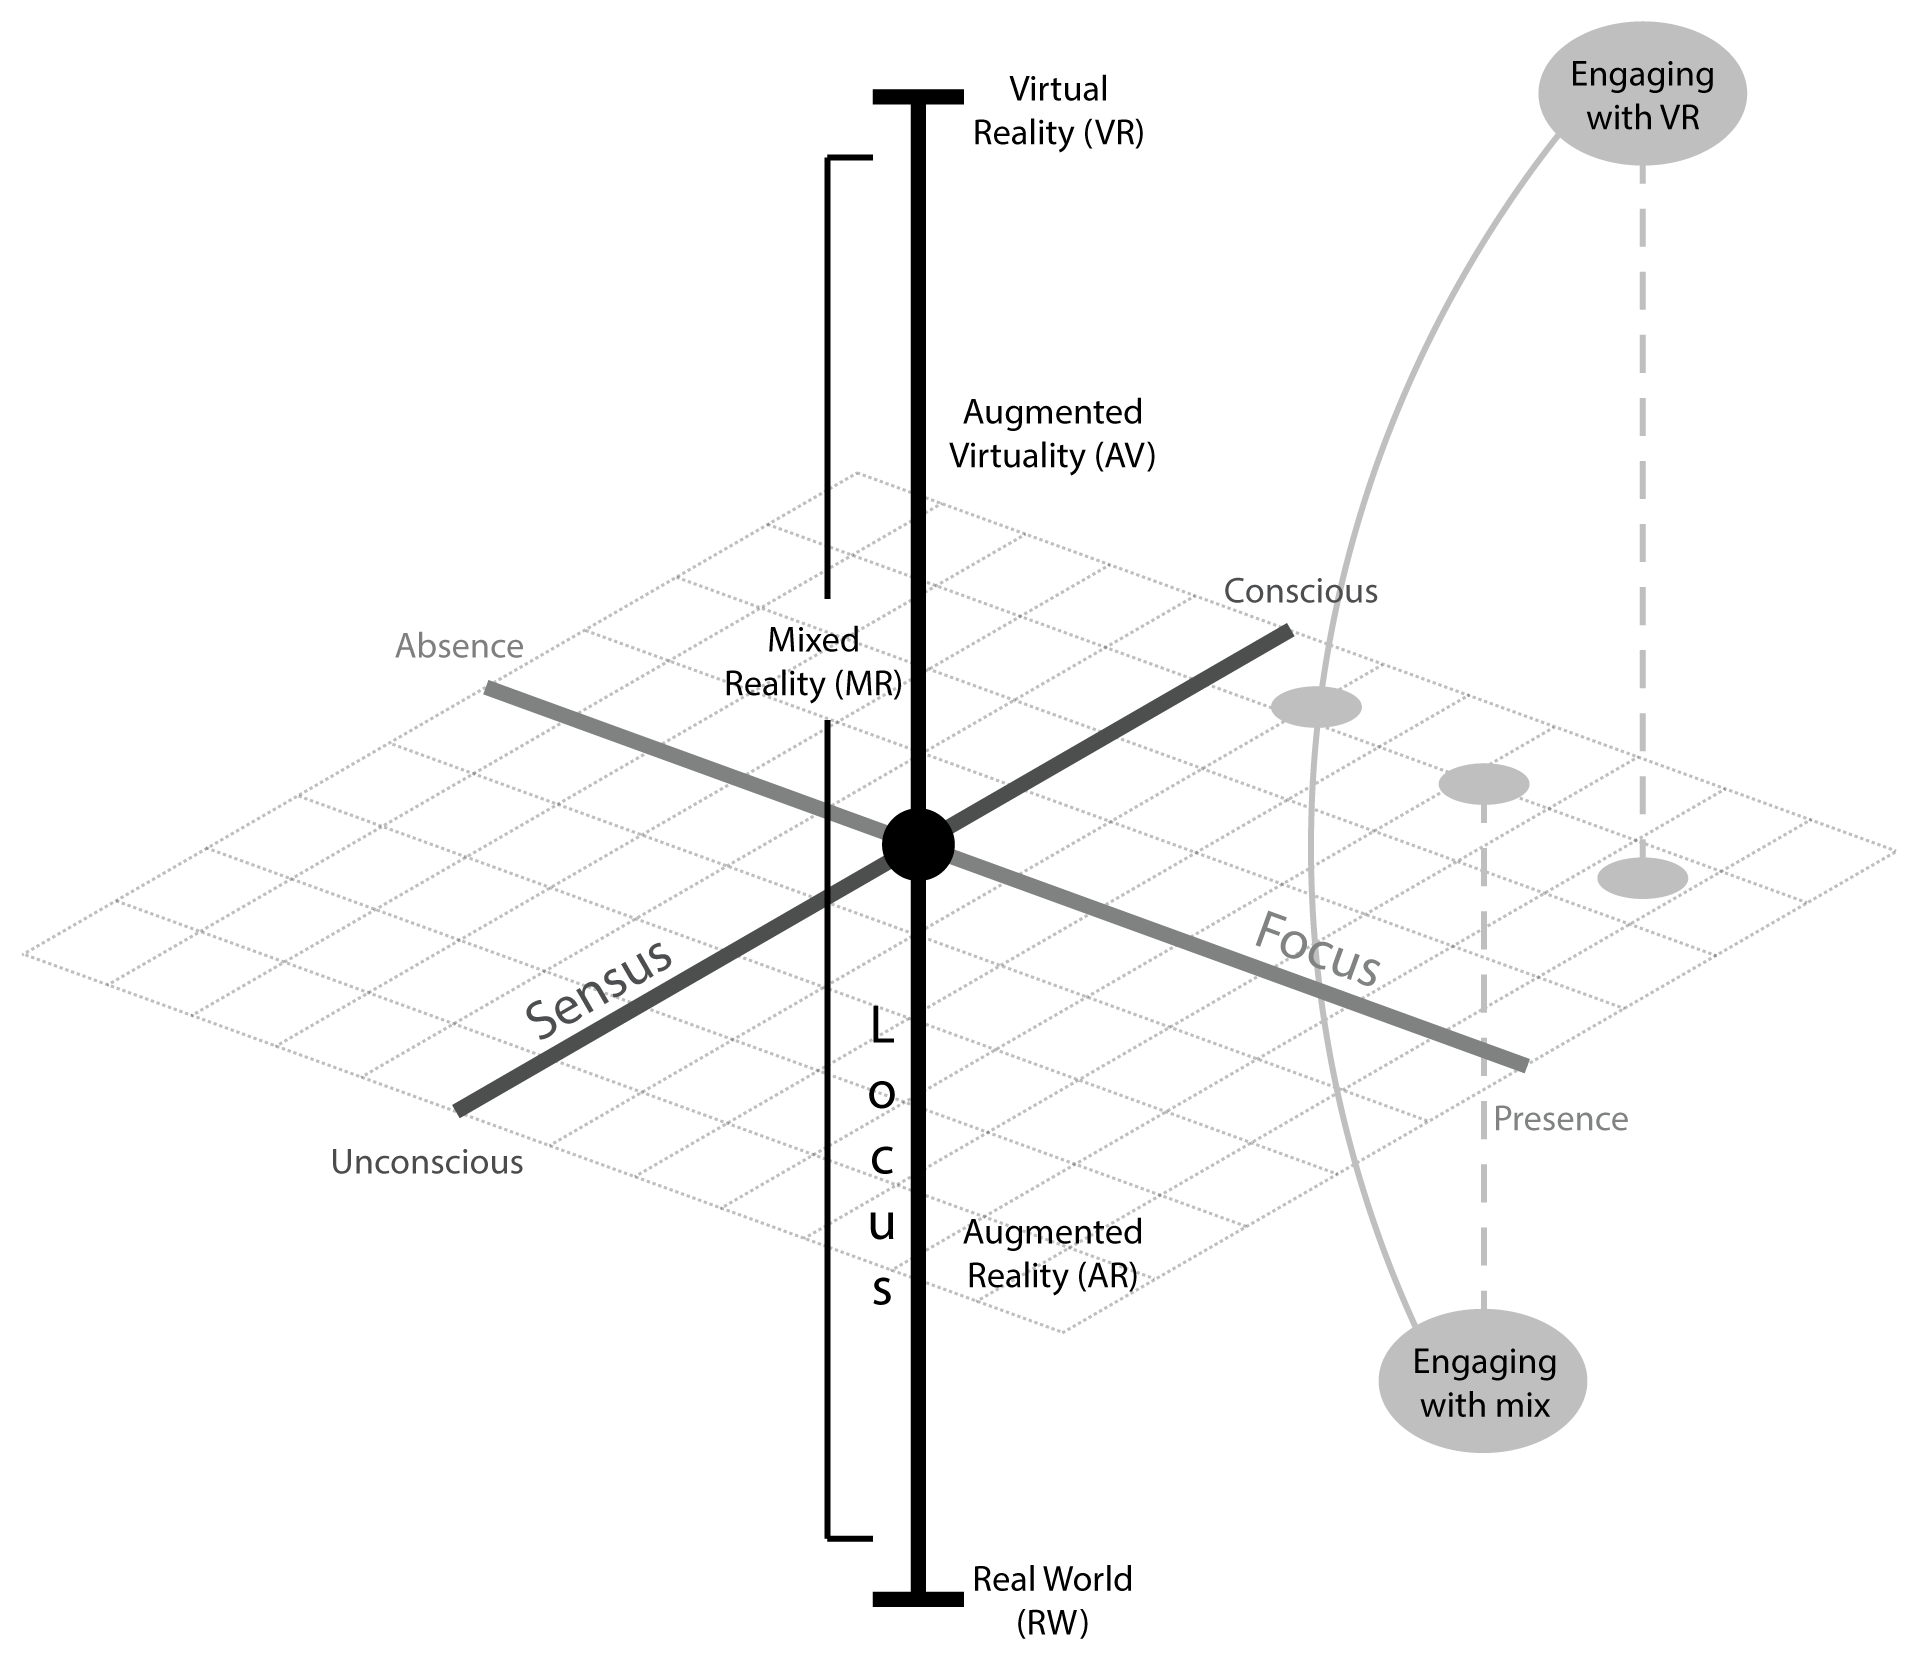
\includegraphics[width=.8\textwidth]{transition-mix-vr.png}
		\caption{Visualisation using the combined Milgram/Waterworth model of the theorised experience of a user of the Mirrorshades parallel reality platform performing a transition between a RW/VR mix and the VR environment.}
		\label{transition-mix-vr.png}
	\end{center}
\end{figure}

The user is expected to experience a greater sense of presence (a position further toward the presence extreme of the focus of attention axis) when engaging with the RW environment in the scenario depicted by figure \ref{focus-locus-sensus-with-virtuality-continuum-with-transition} than when than when engaging with the RW/VR mix in the scenario depicted by figure \ref{transition-mix-vr.png}, as comprehending the mixed environment is expected to require a greater degree of conceptual/abstract reasoning. However in figure \ref{transition-mix-vr.png}, performing a transition to the wholly VR environment is expected to result in a smaller deflection upon the focus of attention axis than performing a transition to VR in figure \ref{focus-locus-sensus-with-virtuality-continuum-with-transition}, as instead of being presented with a completely new environment the user is instead presented with a solidification of the VR environment that they were already perceiving to a lessened extent when engaging with the RW/VR mix.

\newpage

Considering the second aspect, the effect upon breaks in presence is illustrated by once again considering the scenario represented by figure \ref{focus-locus-sensus-with-virtuality-continuum-with-transition} and this time comparing it to that of figure \ref{transition-rw-vr-hard.png}. Figure \ref{focus-locus-sensus-with-virtuality-continuum-with-transition} envisages a transition in which the visual stimuli of one environment are gradually replaced with those of the other, such as by performing linear interpolation upon the opacity of the textures that the camera streams are rendered to. Figure \ref{transition-rw-vr-hard.png} envisages a reaction to the visual stimuli of one environment being instantaneously replaced with those of the other. The instantaneous switch will intuitively come as more of a shock to the user than the gradual exchange, resulting in a worse break in presence and thus the greater deflection upon the focus of attention axis, and also requiring a greater length of time of receiving visual stimuli from the VR environment before coming to understand them.

\begin{figure}[h]
	\begin{center}
		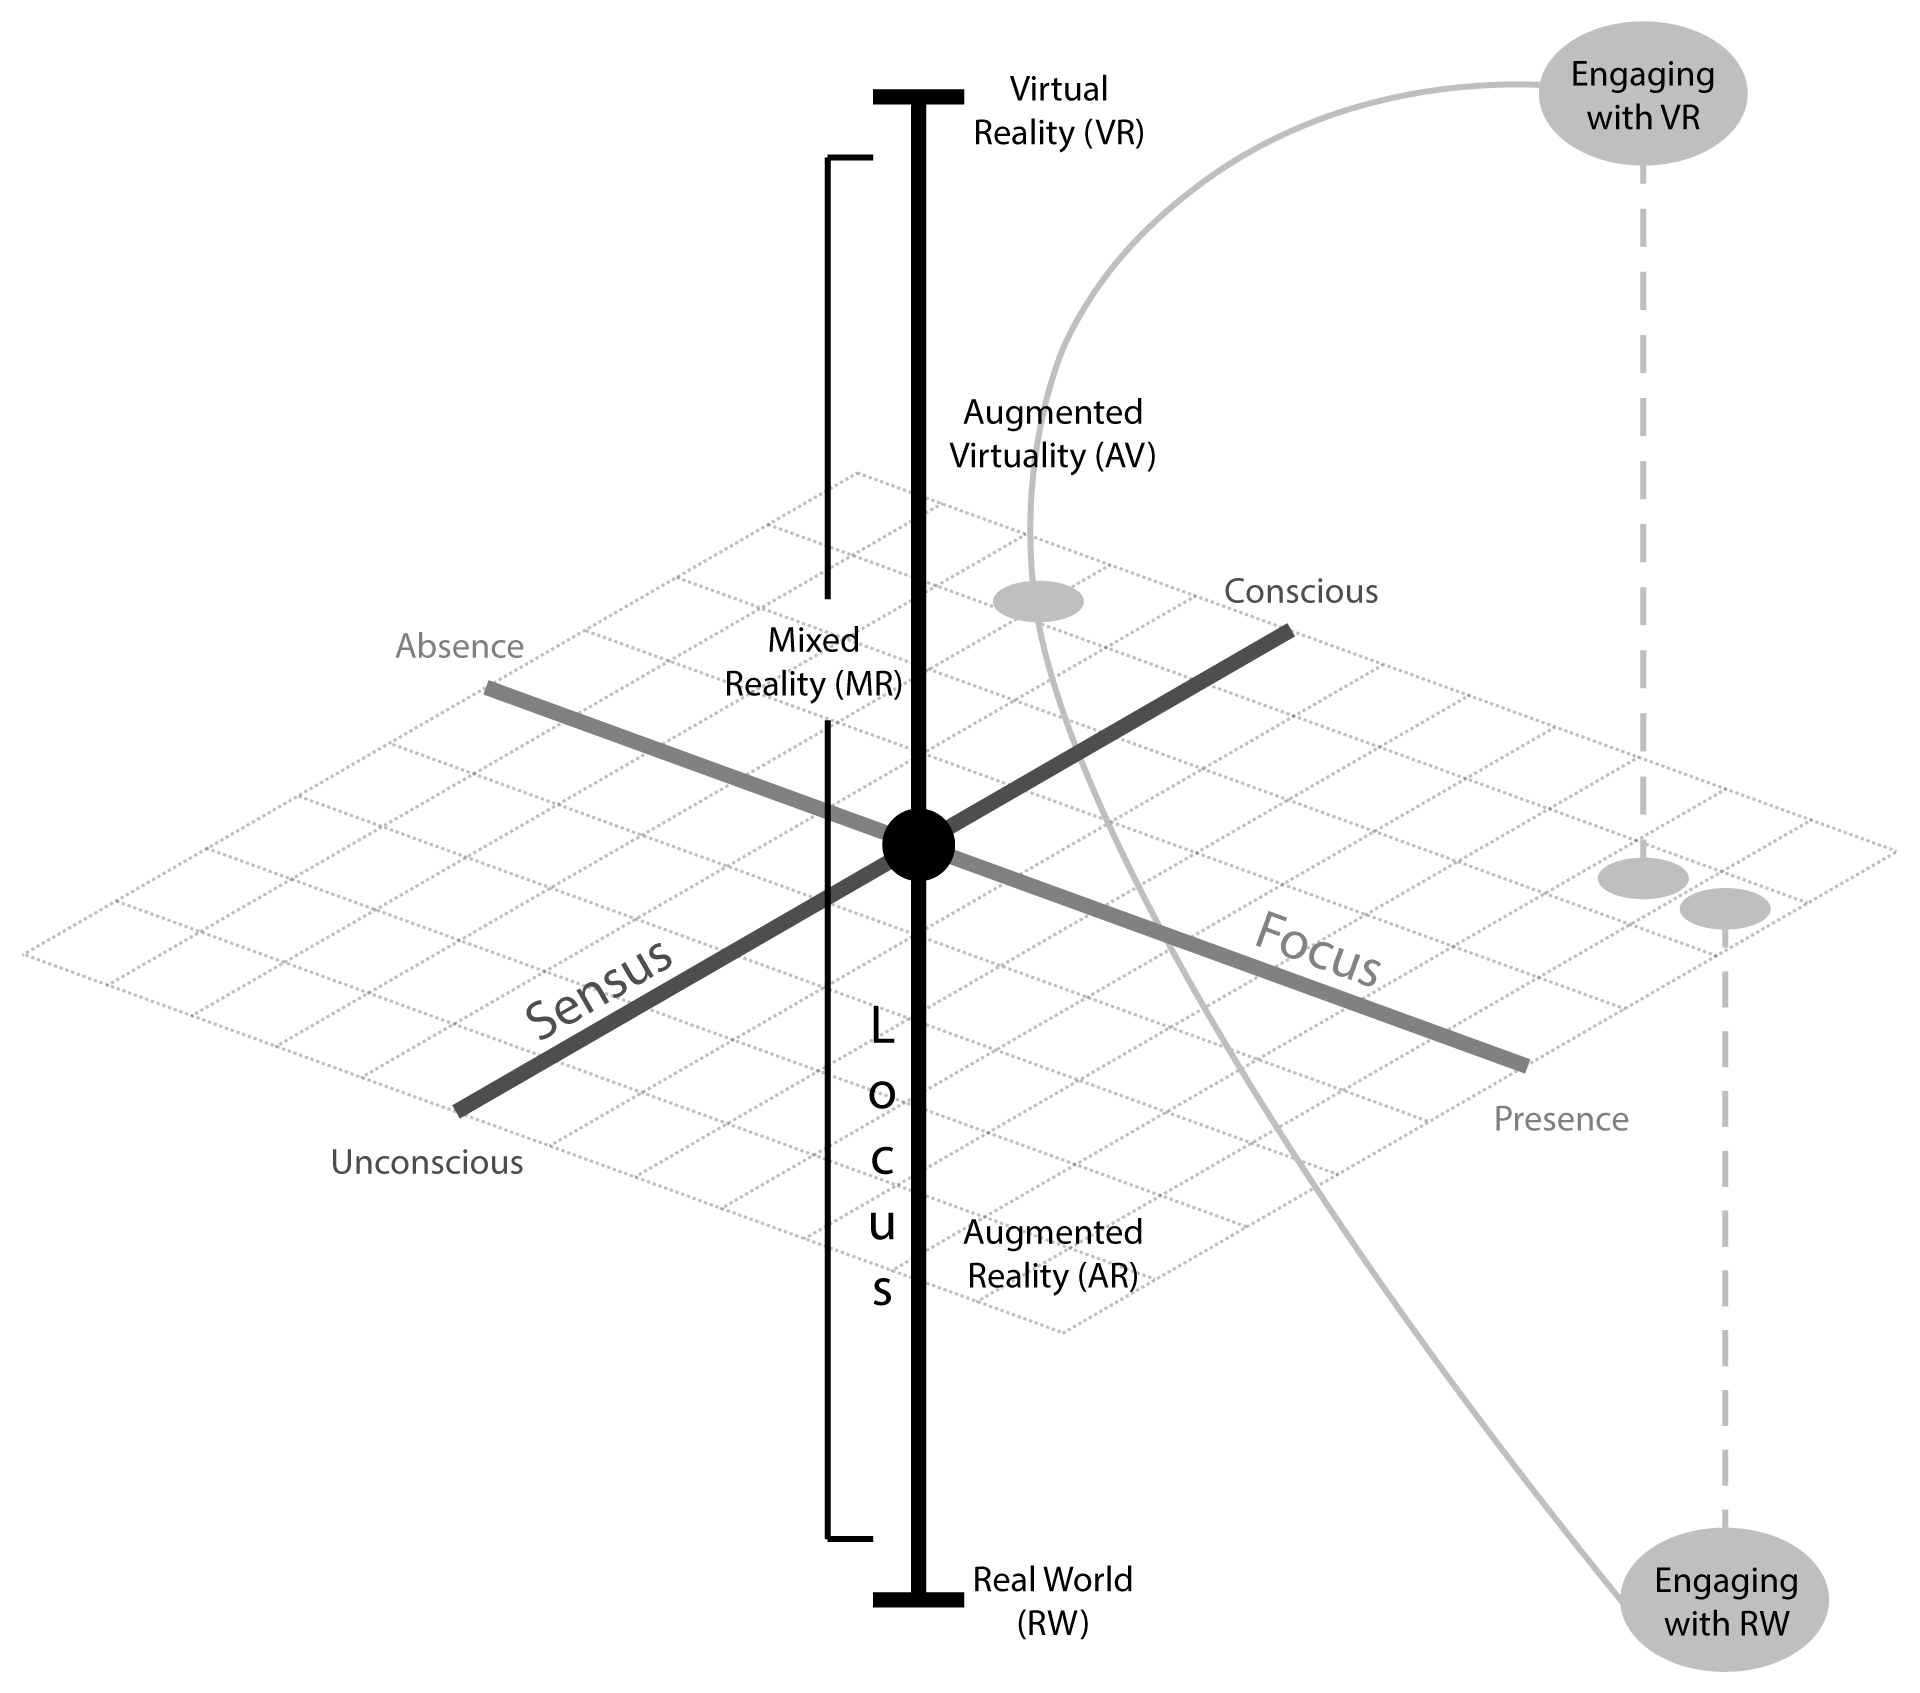
\includegraphics[width=.8\textwidth]{transition-rw-vr-hard.png}
		\caption{Visualisation using the combined Milgram/Waterworth model of the theorised experience of a user of the Mirrorshades parallel reality platform performing an instantaneous transition between its constituent RW and VR environments.}
		\label{transition-rw-vr-hard.png}
	\end{center}
\end{figure}

In order to best implement a parallel reality system that provides its users with the ability to perform transitions like this, ascertaining the optimum manner in which to perform these transitions between the constituent environments is important. As such a number of different transition methods were designed and implemented for evaluation through user studies.

%=========================================================================================================

\newpage

\subsection{Control Mechanism for Transitions}

Granting the user the ability to trigger transitions between different visual stimuli, including the ability to choose different styles of transition, required the user to be provided with a control mechanism. This control mechanism needed to detract as little as possible from the user's ability to process the visual stimuli that they were receiving from the DK1. As the camera solution mounted to the DK1 is not ideal for observing very close objects due to heightened negative parallax at close distances and the roughly arm's length hyperfocal distance (see section \ref{constraints_of_dk1_see_through_solution}), a control modality that could be quickly learned and then used by touch/memory was necessary.

Using the smartphone upon which IndoorAtlas operates did not represent a good solution, as a lack of physical buttons upon modern smartphones meant that triggering different transitions would require touching different areas of the screen - a task that would not be reliably performable without looking at the phone each time. As the smartphone must be held in the user's hand (placing it in a pocket or in the satchel was attempted, however a severe negative impact on the performance of IndoorAtlas was experienced) the control mechanism must be usable with the remaining single hand.

An Xbox 360 controller was thus chosen to accomplish this goal. When held with just the right hand the controller features multiple push buttons and an analogue trigger accessible between the thumb and first finger. These buttons are easily distinguishable from each other via touch due to their layout, while the provision of an analogue trigger allows for user controllable transition speeds and pausing at intermediary positions between constituent environments in addition to simple binary control between two options as granted by the buttons. Pressing one of the buttons or pulling the trigger causes a transition to occur, while releasing the button or trigger causes a return to the default view.

The Leap Motion hand tracking sensor was subsequently used by other researchers in a similar capacity in order to switch between VR and RW visuals when attached to the front of an Oculus Rift DK2, by detecting a hand gesture moving down over its field of view\footnote{\url{http://blog.leapmotion.com/new-demo-switch-vr-real-world-simple-gesture/}}. Whilst this approach does not require the user to hold a controller, distinguishing between multiple different gestures to control different transitions would prove more difficult both in terms of the user learning and correctly performing the gestures and in terms of the platform correctly recognising them. Furthermore, occupying a position between VR and RW in the same manner that the trigger of the Xbox controller allows would require the user to keep their hand in front of the Leap Motion sensor and thus obscure part of the their view of the RW visuals if it were mounted to the DK1 in the style of this subsequent project.

%=========================================================================================================

\section{Transition Types}

Four different styles of transition were implemented for the Mirrorshades platform; three that are manually triggered by the user via the controller and one that occurs automatically at timed intervals. In addition a mode that changes the default view from wholly RW to a mix of RW and VR was implemented. This set of different transitions allowed experimentation with different implementations of both serially and concurrently experienced real and virtual environments in parallel reality systems, exploring both of the conceptual aspects of transitions identified in section \ref{design-considerations-for-rw-vr-transitions}.

%=========================================================================================================

\subsection{Hard transition}
\label{sub-hardswitch}
The user presses and holds the \texttt{[A]} button on the controller to switch the visual stimuli displayed by the DK1 from the default view to VR. When the \texttt{[A]} button is released, the visual stimuli displayed by the DK1 switch back from VR to the default view. This is a `hard' or `immediate' transition with no fading or transition effect. Figure \ref{scenario1} illustrates this scenario while figure \ref{transition-rw-vr-hard.png}, discussed in the previous section, visualises the expected user experience of this transition upon the combined Milgram/Waterworth model (assuming a default environment that is wholly RW).

\begin{figure}[h]
	\begin{center}
		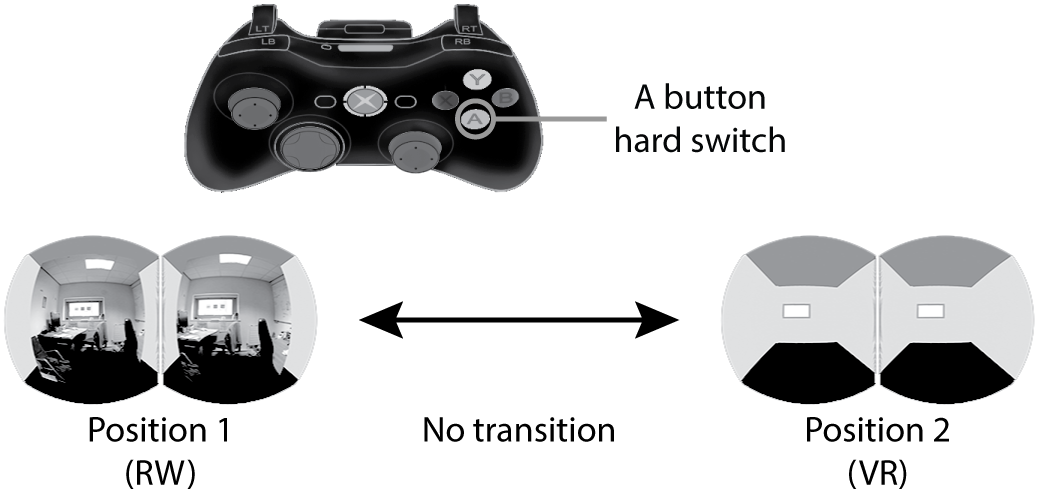
\includegraphics[width=0.5\textwidth]{switching-hard-with-controller.png}
		\caption{Instantaneous hard transition between RW and VR visual stimuli.}
		\label{scenario1}
	\end{center}
\end{figure}

%=========================================================================================================

\subsection{Transition with linear interpolation}
\label{transition-with-linear-interpolation}
The user presses and holds the \texttt{[B]} button on the controller to switch the visual stimuli displayed by the DK1 from the default view to VR. When the \texttt{[B]} button is released, the visual stimuli displayed by the HMD switch back from VR to the default view. This switch fades between the default view and VR visual stimuli (and vice-versa) using linear interpolation on the opacity of the game objects that the camera feeds are rendered upon. Figure \ref{scenario12} illustrates this scenario while figure \ref{focus-locus-sensus-with-virtuality-continuum-with-transition}, discussed in the previous section, visualises the expected user experience of this transition upon the combined Milgram/Waterworth model (assuming a default environment that is wholly RW).

\begin{figure}[h]
	\begin{center}
		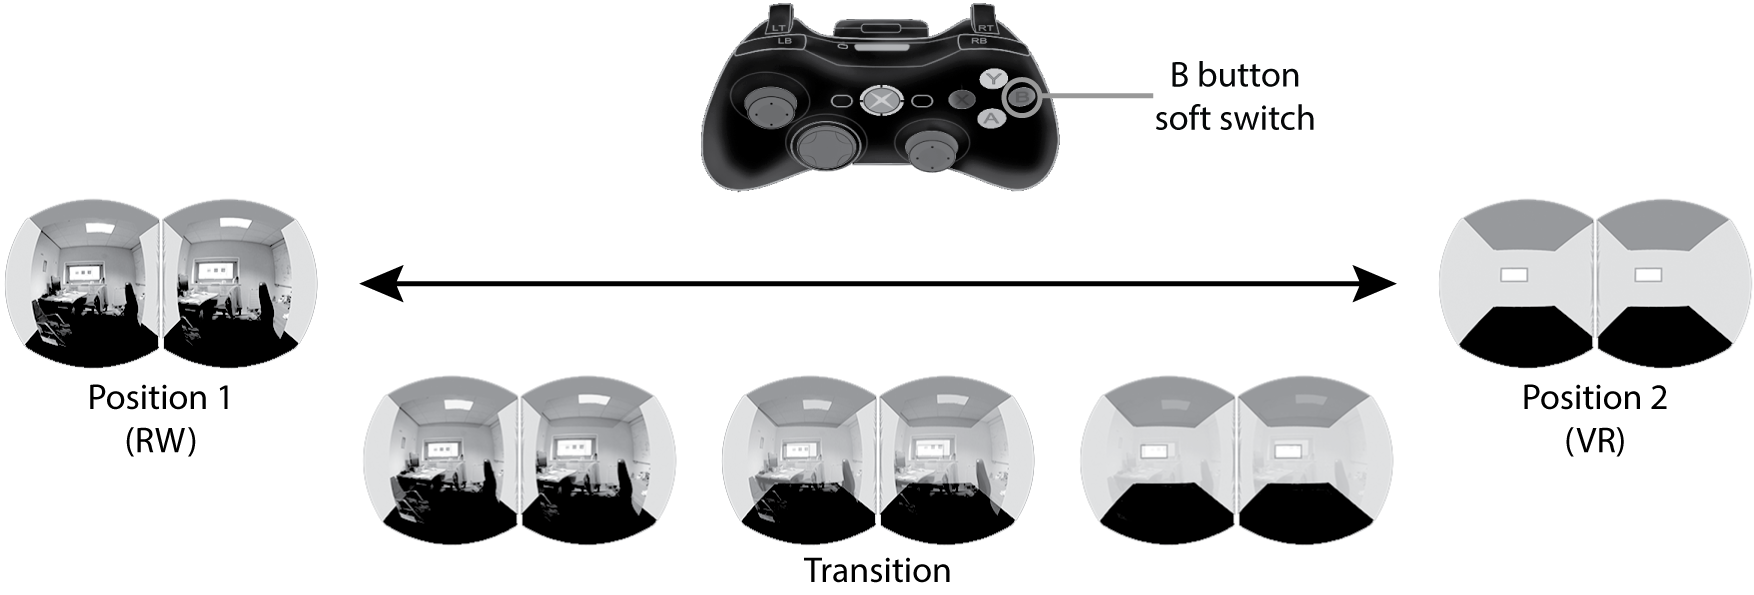
\includegraphics[width=.8\textwidth]{switching-soft-with-controller.png}
		\caption{Transition with linear interpolation between RW and VR visual stimuli.}
		\label{scenario12}
	\end{center}
\end{figure}

%=========================================================================================================

\subsection{Analogue selectable opacity}
\label{analogue-selectable-opacity}
The user pulls the right analogue trigger (\texttt{[RT]}) on the controller and the position of the trigger maps directly to the opacity of the game objects that the camera feeds are rendered upon. The user can choose to stop at any intermediary position that suits their needs, keeping the level of opacity of the camera feeds at that position, as well as controlling the rate at which the visual stimuli from either environment fade by changing how quickly they change their depression of the trigger. Pulling the trigger all the way in displays only visual stimuli from the VR environment, while releasing it completely displays only visual stimuli from the default view. The number of intermediary positions attainable is limited only by the resolution of the trigger and the encoding of the value.

\begin{figure}[h]
	\begin{center}
		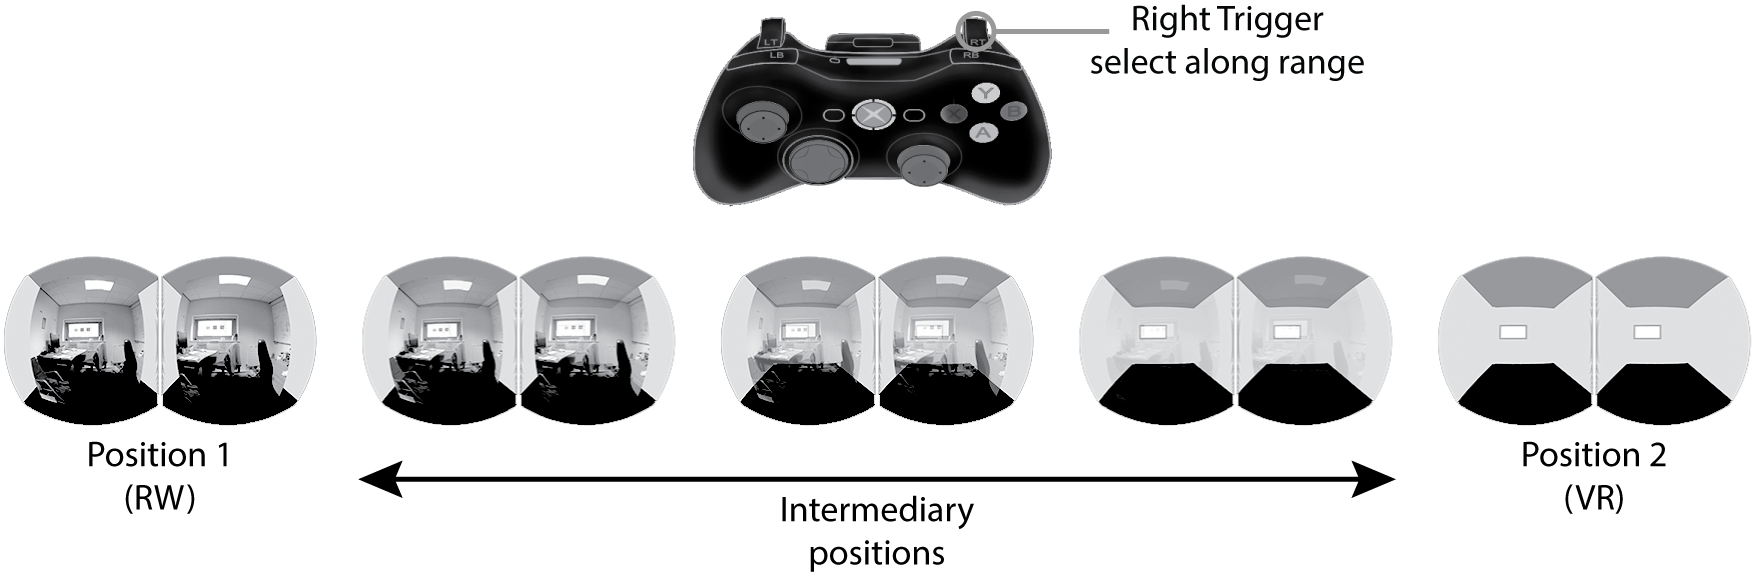
\includegraphics[width=.8\textwidth]{switching-analogue-with-controller.png}
		\caption{Analogue selectable opacity between RW and VR visual stimuli, where any intermediary position can be lingered upon.}
		\label{scenario2}
	\end{center}
\end{figure}

This method allows the user to superimpose VR visual stimuli upon default visual stimuli at any level that they wish, in effect viewing both of the constituent environments of the system concurrently, whereas the previous two transition types present the environments serially. This is similar but not identical to augmented reality, as instead of displaying discrete virtual objects upon the user's view of their RW environment, a \textit{complete} VR environment is superimposed upon their view of the RW environment.

Figure \ref{scenario2} illustrates this scenario, while considering the combined Milgram/Waterworth model this method in essence was expected to allow the user to control the severity of the deflection upon the focus of attention axis by altering the speed at which the oscillation upon the locus of attention axis is performed, to suit their disposition, the current environmental conditions and the task at hand.

%=========================================================================================================

\subsection{Periodic hard transitions}
\label{subsub-periodic}
Independent or in addition to any of the previous transition types, the visual stimuli displayed by the DK1 transition from the default view to VR at a set interval and for a set amount of time. For example, every 3 seconds the stimuli switch from the default view to VR for 0.2 of a second before switching back to the default view. Any user triggered transition causes the interval timer to be reset such that an `automated' transition will never occur after less time from a user triggered transition than the set interval. Automated transitions are disabled whilst \texttt{[RT]} is at all depressed. Figure \ref{scenariotimed} illustrates this scenario, where \texttt{i} represents the interval between switches and \texttt{d} represents the duration of the transition from the default view to VR.

\begin{figure}[h]
	\begin{center}
		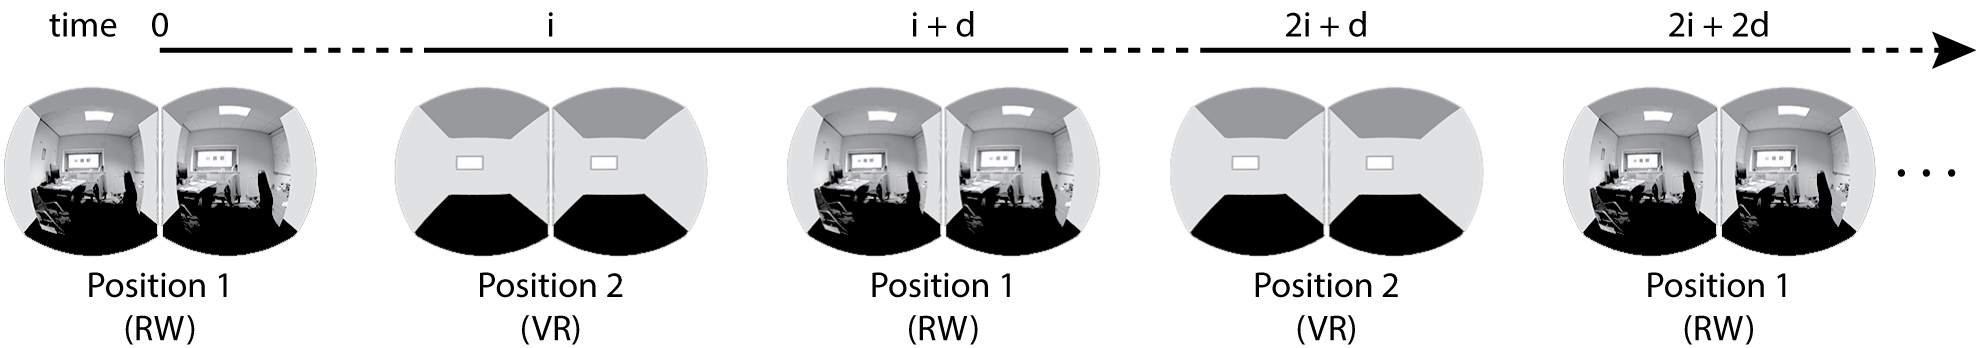
\includegraphics[width=\textwidth]{timed-switch.png}
		\caption{Periodic instantaneous hard transition between RW and VR visual stimuli.}
		\label{scenariotimed}
	\end{center}
\end{figure}

Considering the combined Milgram/Waterworth model, it was postulated that these periodic glimpses of the VR environment would lessen the deflection upon the focus of attention axis when the user subsequently performed a manual transition to VR, as they would perhaps almost subconsciously maintain an awareness of the current state of the virtual environment at all times, even if the duration of the periodic glimpses was not enough to discern particular details. However by keeping the default view as 100\% RW, sensus of attention when viewing the default view was expected not to be drastically affected by the introduction of the periodic switches.

%=========================================================================================================

\subsection{Reduced maximum opacity}
\label{subsub-baseopacity}
Independent or in addition to any of the previous transition types, the maximum opacity of the game objects that the camera feeds are rendered upon is reduced such that the default view displays a mix of VR superimposed upon RW. Figure \ref{scenariobaseopacity} illustrates this scenario in combination with a hard transition (section \ref{sub-hardswitch}) in which the user triggers hard transitions between the default view of the VR/RW mix and a fully VR environment. Figure \ref{transition-mix-vr.png} visualises the expected user experience of this RW/VR mix default view upon the combined Milgram/Waterworth model when combined with a linear interpolated transition (section \ref{transition-with-linear-interpolation}).

\begin{figure}[h]
	\begin{center}
		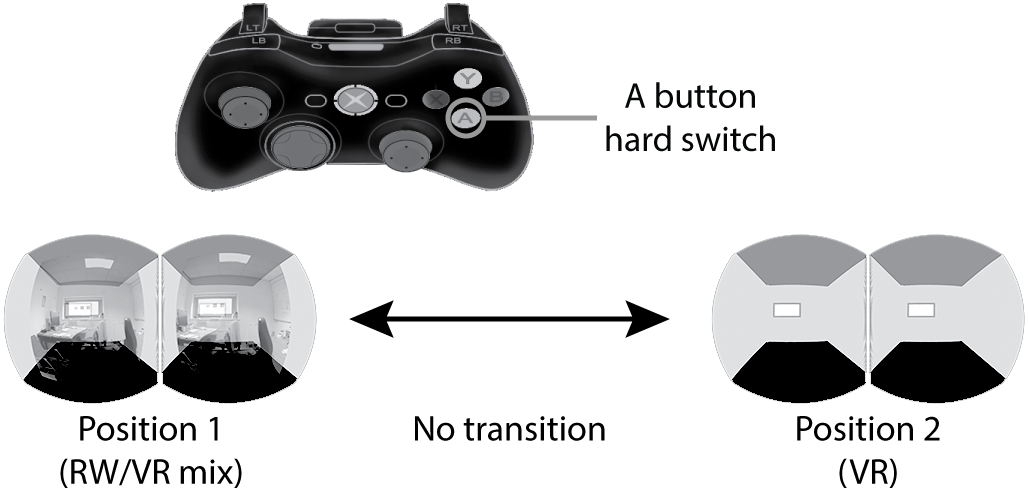
\includegraphics[width=0.5\textwidth]{base-opacity-hard-switch.png}
		\caption{Instantaneous hard transition between RW/VR mix and VR visual stimuli.}
		\label{scenariobaseopacity}
	\end{center}
\end{figure}

Unlike with the periodic hard transition approach (section \ref{subsub-periodic}), which also introduces an aspect of the VR environment to the default view in an attempt to reduce the severity of deflection upon the focus of attention axis when performing a transition, the sensus of attention in this reduced maximum opacity scenario is depicted as being heightened when viewing the RW/VR mix default view. This is because `making sense' of the mixed environment was expected to require more conscious thought than of an environment that is wholly real, even one that is wholly real but interspersed with momentary glimpses of virtual.

%=========================================================================================================

\section{The Assembled Mirrorshades Parallel Reality Platform}

Figure \ref{experimentalimplementation} presents an overview of the individual components and services that made up the Mirrorshades parallel reality platform as employed in user studies at St Salvator's chapel.

\begin{figure}[h]
	%\thispagestyle{empty}
	\begin{center}
		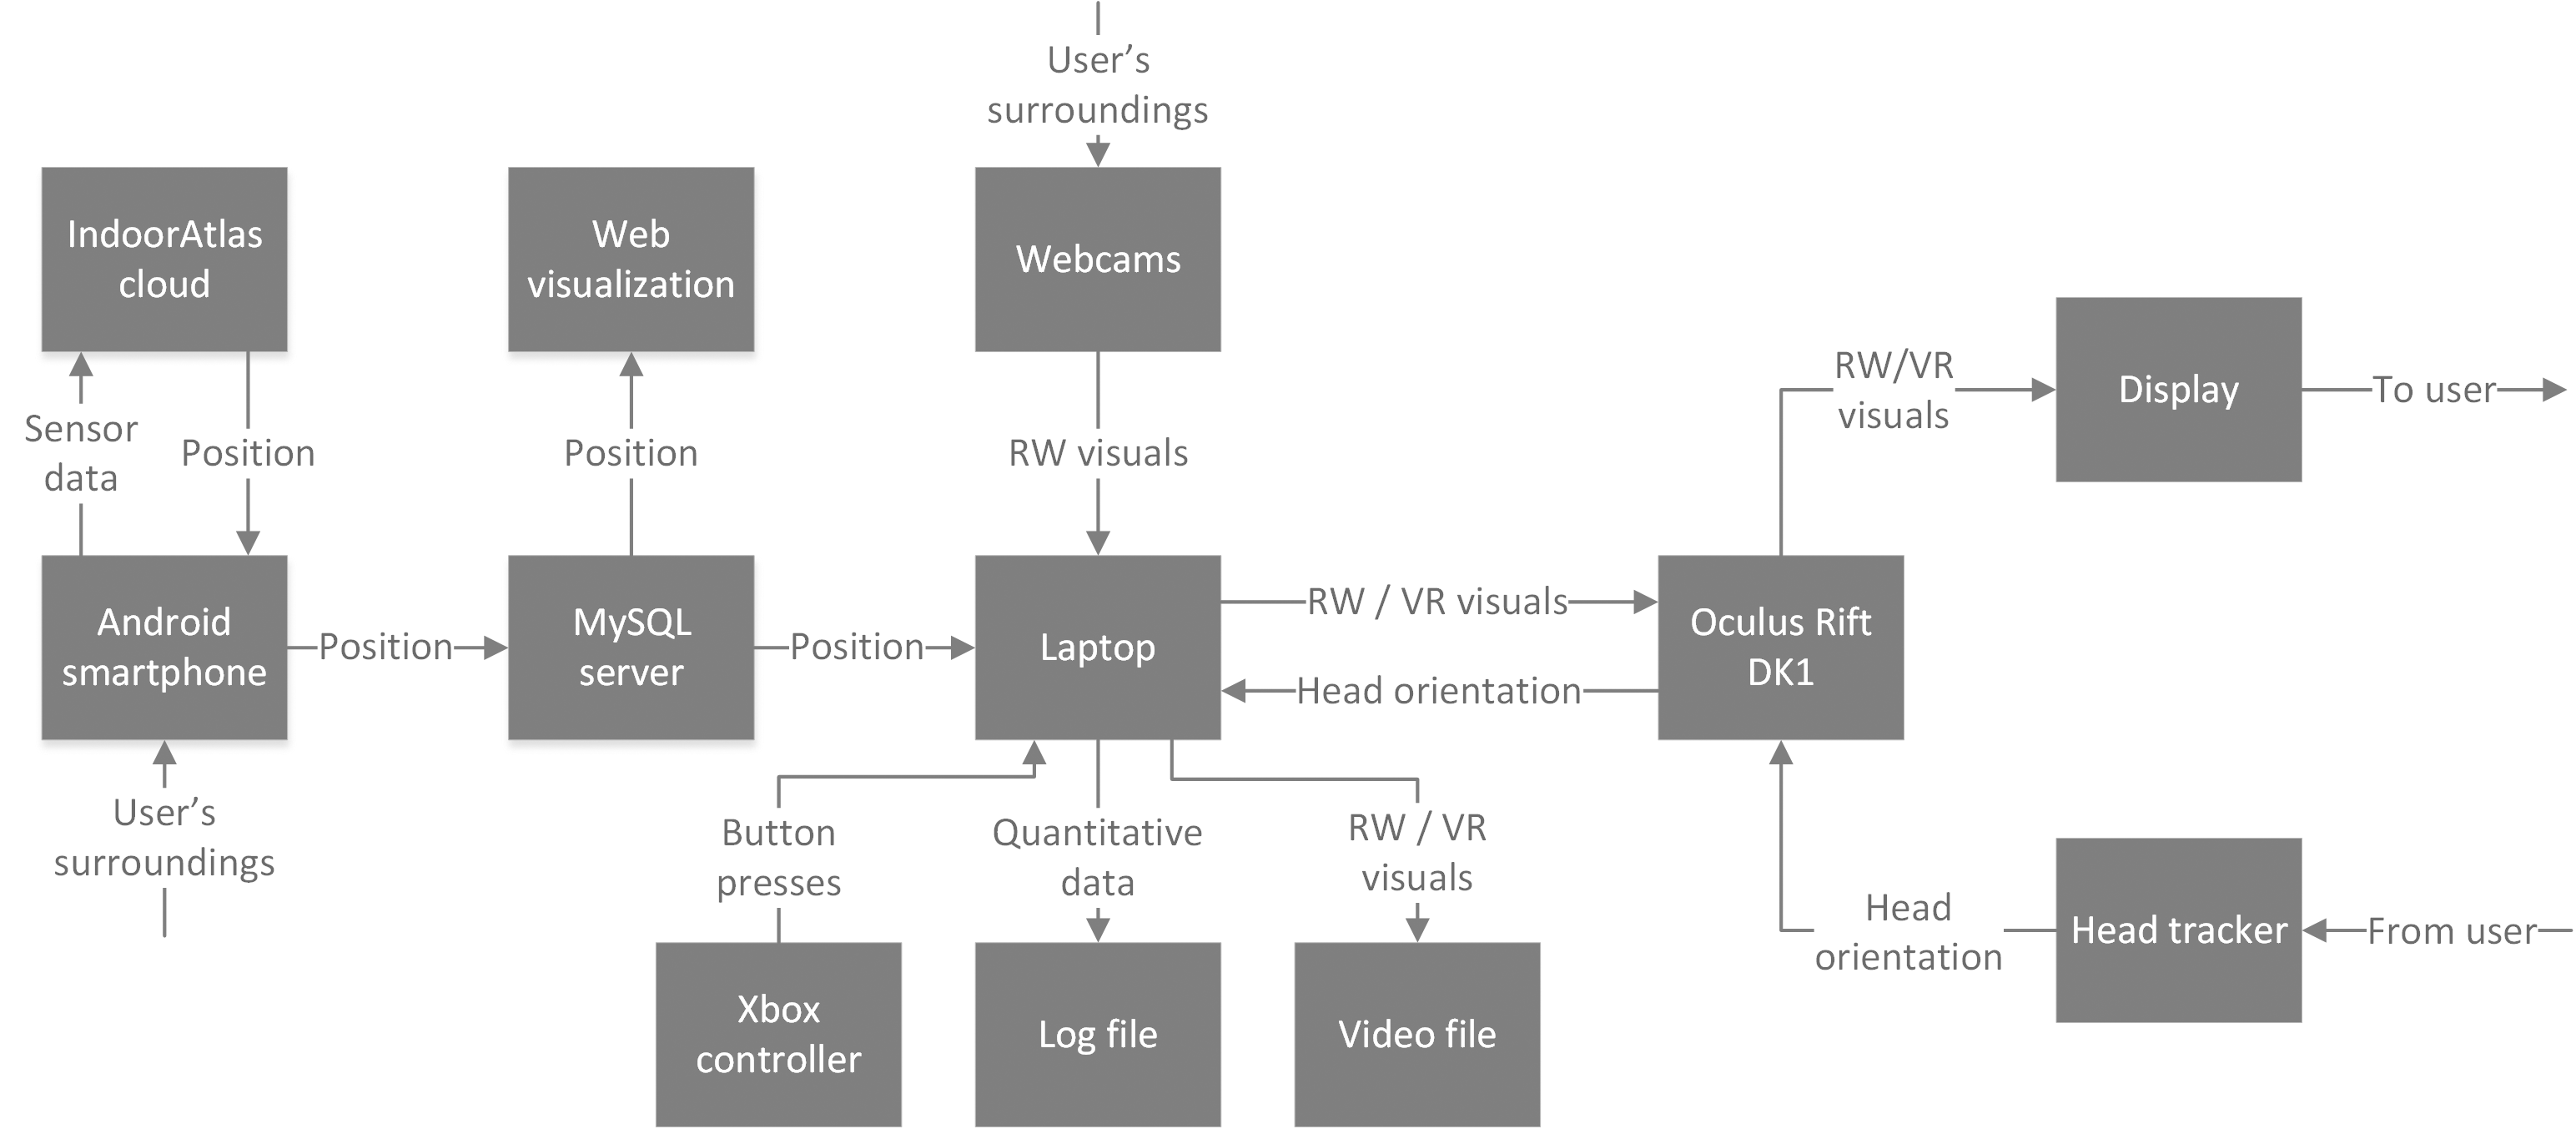
\includegraphics[width=.925\linewidth]{experimental-implementation.png}
		\caption{Implementation of Mirrorshades parallel reality platform.}
		\label{experimentalimplementation}
	\end{center}
\end{figure}

\subsection{Hardware Components}
The hardware components of the system that were carried by the user comprised:
\begin{itemize}
	\item An Oculus Rift DK1 HMD modified by the addition of a stereo camera video see-through solution comprising 2x Logitech C310 webcams modified with S-mount lens mounts and 2.1mm lenses to provide approximately 81.2\textdegree\ horizontal FOV of the RW environment.
	\item A 12,000mAh USB battery pack, capable of outputting 2.1A at 5V, to power the DK1.
	\item A Clevo W110ER laptop computer, with an Intel i7-3632QM four-core/eight-thread processor, Nvidia GT 650M graphics card, 16GiB system memory and a SSD to allow safe operation while moving, running Windows 7 Enterprise.
	\item A Google Nexus 5 smartphone, running Android 4.4.4.
	\item An Xbox 360 wireless controller, with USB receiver.
\end{itemize}

Figure \ref{DSCN0198.jpg} shows an overview of this hardware: the laptop computer is bottom left, the DK1 control box (with USB battery pack, 4-port USB hub and Xbox controller receiver) is bottom right, the DK1 itself (with camera solution attached) is top right, the Xbox controller is top center and the Nexus 5 smartphone is top left. Figure \ref{DSCN0191.jpg} shows a detailed view of the USB battery pack (white, bottom), the DK1 control box (directly above battery), the USB hub (on top, right) and the Xbox controller receiver (top, left). The use of a USB hub allowed there to be only two cables running between the control box bundle and the laptop, which can be seen in figure \ref{DSCN0198.jpg} - the grey cable atop the laptop is the cable from the USB hub and carries the DK1 head tracker information, camera feeds and Xbox controller commands, while the black cable is the HDMI cable that carries visual output from the laptop to the DK1.

\TwoFig{DSCN0198.jpg}{Hardware of the Mirrorshades platform carried by the user.}{DSCN0198.jpg}
       {DSCN0191.jpg}{Detail of Mirrorshades control box bundle.}{DSCN0191.jpg}

The laptop and control box bundle were carried in a satchel worn over the user's shoulder, the smartphone was held in their left hand and the Xbox controller was held in their right hand. In addition to this hardware carried by the user, a remote server was used to provide a MySQL database. During the user studies at St Salvator's chapel the server used had an Intel Xeon E3-1270 four-core/eight-thread processor, 32GiB RAM, 4x WD RE4 1TB hard disks in software RAID6 and 100mbit/s Internet connectivity. This server was running the Debian stable release, with a standard LAMP stack and used mdadm for RAID management.

\subsection{Software Components}
The software components of the system comprised:
\begin{itemize}
	\item An Android application that ran on the Nexus 5 smartphone, determined the location of the smartphone within the building that it was in using IndoorAtlas and submitted these location data via PHP to a database server. The source code of this application is available online\footnote{\url{https://github.com/CJ-Davies/IndoorAtlas_SQL_uploader}}.
	\item A PHP page on the database server that allowed IndoorAtlas position data to be submitted to MySQL.
	\item A MySQL database server that stored location data for the phone and allowed these data to be accessed by any SQL capable client.
	\item Web visualizations of position data held within the MySQL database for both the department building and St Salvtor's chapel (see figures \ref{indooratlas-webpage-jack-cole.png} and \ref{indooratlas-webpage-sallies.png}).
	\item A Unity application that ran on the laptop, combining a virtual model of the building, experienced with the DK1's head tracking, with RW camera streams, controlled via Xbox controller actions and the IndoorAtlas position data polled from the MySQL database server. The Unity project for this application is available online\footnote{\url{https://github.com/CJ-Davies/Mirrorshades}}.
\end{itemize}

Due to the use of a SSD with high transfer rates the video stream sent to the DK1 from the Unity application could be recorded, which by using Nvidia's ShadowPlay\footnote{\url{http://www.geforce.co.uk/geforce-experience/shadowplay}} technology was accomplished without a measurable reduction in framerate of the application. Unlike traditional software video capture solutions such as FRAPS\footnote{\url{http://www.fraps.com/}} which read individual frames from the graphics hardware's back buffer and then encode them using the CPU, ShadowPlay makes use of hardware accelerated support built into the GPU itself to perform the capture and encode process and largely eliminates any overhead.
%=========================================================================================================

\subsection{Execution}
The Unity application hosts the VR representation of the chapel and takes in feeds from both cameras, the DK1 head tracker and the Xbox controller. It also polls the MySQL server for the most recent position data. These inputs are combined together to form the visual output for the DK1 to display to the user. As the user moves their head the visuals that are presented to them upon the DK1's display change accordingly; the RW visuals change due to the cameras being physically fixed to the DK1 and the VR visuals change due to data from the head tracker being used to change the orientation of the virtual cameras in Unity accordingly.

Alignment between RW and VR is achieved by correctly orienting the DK1 before starting the Unity application. The Unity prefab object that encapsulates the avatar functionality has a known virtual origin orientation and knowing this allows the DK1 to be oriented to align the RW and VR visuals (see section \ref{registration-of-camera-and-unity-visuals}).

As the user changes their position by walking, the visuals that are presented to them upon the DK1's display also change accordingly. The RW visuals change due to the cameras' physical attachment to the DK1 whilst the VR visuals change due to the user's position, as reported by the smartphone and IndoorAtlas, being used to move the position of the Unity cameras to the equivalent position within the VR representation. As the user presses buttons or pulls the trigger upon the Xbox controller, the visuals that are presented to them upon the DK1's display transition between RW and VR in different styles depending upon which button/trigger was activated.

%=========================================================================================================

\section{Initial Testing}
\label{initial-testing}
The complete Mirrorshades platform was initially tested within the department building (a video of which can be viewed online\footnote{\url{https://www.youtube.com/watch?v=oy5NqqDtkJ4}}) as shown in figures \ref{testing-vids-screenshots/jc-1.png} and \ref{testing-vids-screenshots/jc-2.png}. Note that this test took place with an earlier PS3 Eye based camera solution before the camera feeds had been correctly scaled. This initial integration test confirmed the correct functioning of the platform as a whole and that the accuracy of the IPS was great enough for the desired modality of interaction, at least within the department building with its abundance of metal building materials and electrical provisions.

\TwoFig{testing-vids-screenshots/jc-1.png}{Mirrorshades test in department building (real).}{testing-vids-screenshots/jc-1.png}
       {testing-vids-screenshots/jc-2.png}{Mirrorshades test in department building (virtual).}{testing-vids-screenshots/jc-2.png}

%\TwoFig{testing-vids-screenshots/jc-3.png}{Mirrorshades test in department building.}{testing-vids-screenshots/jc-3.png}
%       {testing-vids-screenshots/jc-4.png}{Mirrorshades test in department building.}{testing-vids-screenshots/jc-4.png}

The first test in St Salvator's chapel (a video of which can be viewed online\footnote{\url{https://www.youtube.com/watch?v=W4oPIHIr9Z4}}) as shown in figures \ref{testing-vids-screenshots/sallies-first-1.png} and \ref{testing-vids-screenshots/sallies-first-2.png}, confirmed that the accuracy of the IPS within the chapel was also sufficient and that the wireless network provision within the chapel was of sufficient speed and stability to support the operation of the platform. By this point the camera feeds had had correct scaling applied to them, thus the `narrower' appearance of the images in figure \ref{testing-vids-screenshots/sallies-first-1.png} than in figure \ref{testing-vids-screenshots/jc-1.png}.

\TwoFig{testing-vids-screenshots/sallies-first-1.png}{Mirrorshades test in St Salvator's chapel (real).}{testing-vids-screenshots/sallies-first-1.png}
       {testing-vids-screenshots/sallies-first-2.png}{Mirrorshades test in St Salvator's chapel (virtual).}{testing-vids-screenshots/sallies-first-2.png}

\newpage

Testing then took place with members of the Open Virtual Worlds research group (a video of which can be viewed online\footnote{\url{https://www.youtube.com/watch?v=pvGV5dCjt4U}}) as seen in figures \ref{testing-vids-screenshots/sallies-second-1.png} to \ref{testing-vids-screenshots/sallies-second-8.png}. These tests provided initial feedback from participants not directly involved with development of the platform. During these early tests there was a strong preference expressed from the participants toward the transition with linear interpolation (see section \ref{transition-with-linear-interpolation}).

\TwoFig{testing-vids-screenshots/sallies-second-1.png}{Mirrorshades test with OVW group members in St Salvator's chapel (composite, 1/4).}{testing-vids-screenshots/sallies-second-1.png}
       {testing-vids-screenshots/sallies-second-4.png}{Mirrorshades test with OVW group members in St Salvator's chapel (composite, 2/4).}{testing-vids-screenshots/sallies-second-4.png}

%\TwoFig{testing-vids-screenshots/sallies-second-5.png}{Mirrorshades test with OVW group members in St Salvator's chapel.}{testing-vids-screenshots/sallies-second-5.png}
%       {testing-vids-screenshots/sallies-second-6.png}{Mirrorshades test with OVW group members in St Salvator's chapel.}{testing-vids-screenshots/sallies-second-6.png}

\TwoFig{testing-vids-screenshots/sallies-second-7.png}{Mirrorshades test with OVW group members in St Salvator's chapel (composite, 3/4).}{testing-vids-screenshots/sallies-second-7.png}
       {testing-vids-screenshots/sallies-second-8.png}{Mirrorshades test with OVW group members in St Salvator's chapel (composite, 4/4).}{testing-vids-screenshots/sallies-second-8.png}

%=========================================================================================================

\section{Summary}
This chapter has recounted the development of the Mirrorshades parallel reality platform, which combines the Oculus Rift DK1 VR HMD with the IndoorAtlas IPS. The greater positional accuracy of the IPS compared to the GPS solution used within the VTW project allows investigation into the freeform exploration scenario and into aspects of the detailed comparison scenario. The immersive nature of the DK1, completely filling the user's FOV with mediated stereoscopic visuals, allows for investigation of the experiential aspect of switching wholly between complete and discrete real and virtual environments that was originally envisioned of the parallel reality concept but not realised by the VTW platform's modality of interaction. Four different styles of transition between real and virtual stimuli were implemented and their expected user experience illustrated using the combined Milgram/Waterworth model.

Latency measurements of the video see-through solution were performed and while higher than published best practices for VR experiences they were not expected to be as detrimental to user experience in the style of interaction envisioned of the platform as they would be in more traditional VR gaming scenarios. Initial testing of the platform was conducted, first within a department building and then within St Salvator's chapel, which was introduced as an ideal real world location at which to perform a user study of the Mirrorshades platform within the field of virtual heritage.

%=========================================================================================================